%%% Local Variables: 
%%% mode: latex
%%% TeX-master: t
%%% End: 

\chapter{利用Higgs衰变到双轻子加双光子末态来寻找类轴子}

\section{引言}

在CERN的LHC上,ATLAS和CMS合作组于2012年宣布发现了希格斯(Higgs)粒子~\cite{HiggsdiscoveryAtlas, Chatrchyan:2012ufa, Chatrchyan:2013lba},随后合作组进行了精确的测量~\cite{Hzz_xsec_13,Hzz_xsec_13_v2, Hgg_properties_13_v2, Sirunyan:2021fpv,ttH_13,ttH_13_v2,Hww_diff_13,CMS_mass,ATLAS_mass,ATLAS_xsec,Aaboud:2017vzb,Khachatryan:2016vau}以揭示可能偏离粒子物理标准模型(SM)预测的偏差~\cite{CMS_ALP_3}。比较特别的是,希格斯粒子衰变宽度的偏差或者任何奇异衰变模式的发现都将构成超出标准模型(BSM)新物理的证据。

类轴子模型最初被提出来是用以解决强CP问题~\cite{PhysRevLett.38.1440}。最近,人们发现类轴子可以解释实验上观测到的缪子反常磁矩~\cite{PhysRevLett.119.031802}。类轴子模型利用了有效场论对类轴子和标准模型粒子之间的相互作用进行了描述,特别是对于希格斯粒子,理论预言了希格斯粒子、Z玻色子和类轴子之间的耦合。到目前为止,ATLAS和CMS合作组分别对类轴子的不同产生模式和衰变过程进行了寻找~\cite{CMS_ALP_3, atlas2022search, aad2021measurement, atlas_ALP_2, atlas_ALP_3, CMS_ALP_1, cms2022search}。在本分析中,我们对希格斯粒子衰变到一个Z玻色子和一个类轴子进行了寻找,其中Z玻色子衰变到一对电子或者缪子,类轴子衰变为一个光子对。这样的双轻子加双光子末态具有非常低的标准模型截面这一特征,也为类轴子的寻找提供了不同衰变道的测量结果。同时,这也是在LHC上对希格斯粒子衰变到双轻子加双光子末态的首次测量。图~\ref{fig:Feyman}展示了此过程占主要贡献的费曼图。

\begin{figure}[htbp]
  \begin{center}
	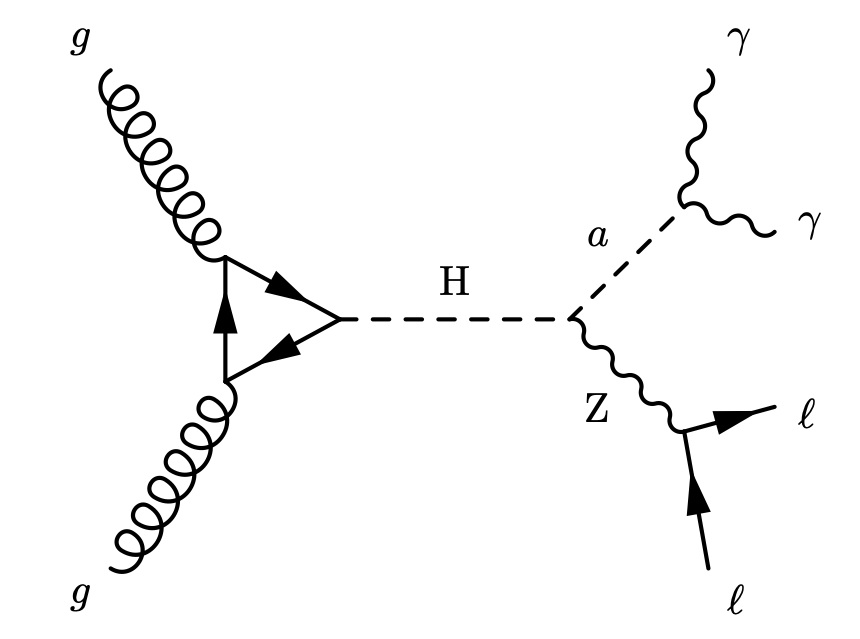
\includegraphics[width=0.45\textwidth]{Thesis (Version 2246)/figures/chapter04/Feyman_diagram.png}
    \bicaption{\quad \centering 希格斯玻色子BSM衰变为一个Z玻色子和一个轻赝标量玻色子,随后分别衰变为两个轻子和两个光子的费曼图}{\quad \centering Feynman diagram for a BSM decay of the H boson into a Z boson and a light pseudoscalar boson, subsequently decaying to two leptons and two photons, respectively}
    \label{fig:Feyman}
\end{center}
\end{figure}

由于我们假设Z玻色子和类轴子都是在壳(On-shell)的粒子,动力学所允许的类轴子质量范围为$m_{a}<m_{H}-m_{Z}\approx35\GeV$,其中,$m_H$和$m_Z$分别为希格斯粒子质量和Z玻色子质量。而对于质量低于1$\GeV$的类轴子,衰变产生的两个光子在探测器中不再能够被区分。因此,本分析只考虑了类轴子的质量范围为$1 < m_{a} < 30\GeV$。

本章结构如下,第\ref{sec:MCData}节介绍了本分析所使用的数据和模拟样本的信息,第\ref{sec:Trigger}节介绍了触发的选择,第\ref{sec:EventReco}节介绍了本分析中所使用的粒子重建,第\ref{sec:EventSelect}节介绍了对信号事例的筛选,第\ref{sec:BDT}节论述了利用参数化的多变量分析的方法提高信号显著度,第\ref{sec:Fit}节介绍了信号提取过程中所使用的统计学方法,第\ref{sec:Bkg}节介绍了本分析中对本底过程的建模,第\ref{sec:Sig}节介绍了对信号过程的建模,第\ref{sec:Sys}节详细介绍了本分析中所涉及的系统误差,最后第\ref{sec:Result}节给出了分析结果。

\section{数据和模拟样本}\label{sec:MCData}

本分析使用了CMS探测器在整个Run2运行期间收集到的质子-质子对撞数据,主要包括探测器于2016年、2017年和2018年间收集的数据,对应的质心能量为13~\si{TeV},三年总的积分亮度为138~\si{fb^{-1}}。本分析所使用的事例模拟和重建都基于CMS合作组开发的软件框架,名为CMSSW。根据探测器运行时期发生的不同情况,对应的分析软件框架会有实时的更新以应对这些变化,因此CMSSW衍生出来了众多版本。本分析所使用的分析框架正是基于CMSSSW\_10\_6\_26,使用的数据版本为Ultra-Legacy,简称UL。

在2016年的探测器运行取数期间,大量硅微条探测器中的高能沉积导致了前端芯片APV25出现短暂的过饱和,使得探测器的读出系统中出现了显著的死时间(Dead-time)。为了解决这个问题,CMS探测器在此后的取数中添加了前向放大器反馈电压偏置(Preamplifier Feedback Voltage Bias,VFP),并对之前收集到的数据进行了修正。因此,在UL版本的数据中,2016年的数据被分为了pre-VFP和post-VFP两部分,其中pre-VFP部分又被称为2016APV。

对于信号样本,本分析利用了MADGRAPH5\_aMC@NLO产生子~\cite{alwall2014automated, Alwall:2007fs, Frederix:2012ps}产生了领头阶的$pp\rightarrow \HZa$信号样本。样本包括CMS实验整个run2三年的数据(2016年、2017年和2018年),针对每年都产生了14个具有不同类轴子质量的信号样本:1到10$\GeV$之间以1$\GeV$为步长,共10个质量点;10到30$\GeV$之间以5$\GeV$为步长,共4个质量点。在模拟中,希格斯粒子的质量被设置为125$\GeV$,并且只考虑了占主导的胶子融合的希格斯产生模式。其他希格斯产生模式对最终结果的贡献仅占1\%,因此可以忽略不计。

本分析中的主要本底过程来自于标准模型Drell-Yan过程产生的一个Z玻色子和喷注,在这个过程中喷注被误判为光子而成为双轻子和双光子末态的本底。为了进一步优化筛选条件,本分析也利用了MADGRAPH5\_aMC@NLO~\cite{alwall2014automated, Alwall:2007fs, Frederix:2012ps}在领头阶对其进行了模拟。由于本分析所涉及的末态属于稀有过程,直接使用MC模拟本底存在非常大的统计误差,因此在最终的信号提取过程中,本底模型通过直接拟合数据的分布得到,MC本底样本仅用于优化筛选条件。

模拟中的部分子分布函数(Parton Distribution Functions,PDFs)使用的是NNPDF3.1~\cite{Ball:2017nwa},部分子的簇射和强子化利用了PYTHIA 8.230产生子~\cite{Sjostrand:2014zea}进行模拟。为了使模拟样本能够和实验数据相符合,我们还需要相应的调节(Tune),对于三年所有的模拟,使用的tune都是CP5~\cite{Khachatryan:2015pea, Sirunyan:2019dfx}。对于CMS探测器的模拟使用的是GEANT4软件\cite{agostinelli2003geant4, 1610988}。附录~\ref{app:data_lists}列出了本分析所使用的所有数据、信号和本底样本。

\section{触发}\label{sec:Trigger}

对于感兴趣的事例,本分析采用了两级触发系统~\cite{Khachatryan:2016bia}。其中,一级触发就是所谓的硬件触发,由CMS探测器中的硬件利用量能器和缪子探测器中的信息,在大约4~\si{\us}的时间间隔内将事例的筛选率由40~\si{\MHz}降低到大约100~\si{\kHz}。二级触发又被称为高级触发,由针对运行速度优化过的事例重建软件所构成,最终可以将事例的筛选率降低到大约1~\si{kHz}。

由于本分析的末态中含有两个由Z玻色子衰变产生的电子或者缪子,因此可以选择单轻子或者双轻子的触发作为本分析的触发。附录~\ref{app:trigger_lists}列出了本分析所使用的所有触发列表。对于单轻子触发,要求电子的最低横动量为25$\GeV$,缪子的最低横动量为20$\GeV$;对于双电子触发,要求两个电子的最低横动量分别为12$\GeV$和14$\GeV$;对于双缪子触发,要求两个缪子的最低横动量分别为8$\GeV$和17$\GeV$;对于一个电子和一个缪子的触发,要求电子的最低横动量为17$\GeV$,缪子的最低横动量为8$\GeV$。

\section{物理对象的筛选以及效率测量}\label{sec:EventReco}

由于对撞中堆积事例的存在,使得每次对撞都会产生许多对撞顶点。在本分析中,事例的初级对撞顶点选为硬散射程度最高的顶点。此外,由于衰变末态中存在两个电子或者缪子以及两个光子,因此对电子、缪子和光子的重建筛选对本分析具有重要的意义。

\subsection{电子筛选}

对电子的重建在第~\ref{subsec:EGReco}节已经有过介绍,电子候选者通过对径迹和簇射的对应观测量进行宽松筛选(Loose cut)得到,目的是为了能够尽可能高的保留电子的事例率,同时也可以排除掉一部分QCD本底。在本分析中,我们对宽松的电子(Loose electron)定义为:电子的横向动量$\mathrm{p_{T}^{e}}>7\GeV$,重建范围为$|\eta^{e}|<2.5$,并且满足宽松的初级顶点限制(重建顶点在横向平面的位移$d_{xy}<0.5~\si{\cm}$、重建顶点在束流方向的位移$d_{z}<1~\si{\cm}$)。

在筛选出loose电子后,为了进一步筛选出纯度更高的电子,本分析采取了多变量分析的辨别方法。对电子的辨别由运行在梯度提升(Gradient Boosting)框架上的机器学习算法来实现,这个算法利用了一些来自电磁量能器、簇射和电子轨迹之间的匹配度、径迹测量以及粒子流隔离度求和等信息作为输入变量对模型进行训练,同时梯度提升框架也保证了训练出来的模型具有非常好的泛化能力。而后将训练结果应用于数据,进而筛选出纯度更高的电子。本分析所使用的训练模型由CMS实验$H\rightarrow ZZ\rightarrow 4\ell$物理分析组~\cite{cmsHZZ}提供,表格~\ref{tab:ele_ID_input_variables}列出了训练模型所使用的输入变量。利用各个电子的这些变量作为模型的输入,可以得到与之对应的输出分数(Output score),然后再对output score进行阈值筛选进而可以得到纯度更高的电子。表格~\ref{tab:ele_ID_WP}列出了不同年份、不同横动量范围和不同$\eta$范围的电子提升决策树输出分数阈值,所有提升决策树输出分数大于这些阈值的电子被保留下来,并称这些电子为严格的电子(Tight electron)。


\begin{table}[h!]
\scriptsize
    \centering
    \bicaption{\quad \centering 电子识别分类器的输入变量概述}{\quad \centering Overview of input variables to the electron identification classifier}
    \resizebox{\textwidth}{!}{
    \begin{tabular}{cl}

\hline %----------------------------------------------------------------------------------------
%\multicolumn{4}{|c|}{Datasets}                                                                \\
观测量类型    &  观测量名称      	\\
\hline %----------------------------------------------------------------------------------------

\multirow{6}{*}{簇射形状变量}
	&  沿$\eta$和$\varphi$方向的能量晶体数谱的标准差:$\sigma_{i\eta i\eta}$,$\sigma_{i\varphi i\varphi}$		\\
	&  超级簇射在$\eta$和$\phi$方向的宽度		\\
	&  位于电子超级簇射之后的强子量能器所沉积的能量和超级簇射能量的比值:$H/E$			\\
	&  环状变量:$(E_{5\times5} - E_{5\times1})/E_{5\times5}$			\\
	&  超级簇射中种子和相邻晶体能量的总和:$R_{9}$			\\
	&  对于端盖部分电子的训练,预簇射中的沉积能量所占总能量的比例:$E_{PS}/E_{raw}$			\\
\hline
\multirow{2}{*}{径迹--簇射匹配度变量}
	& 能量--动量匹配度:$E_{tot}/p_{in}$, $E_{ele}/p_{out}$,$1/E_{tot} - 1/p_{in}$ 			\\
	& 位置匹配度:$\Delta\eta_{in}$, $\Delta\varphi_{in}$,$\Delta\eta_{seed}$			\\
\hline
\multirow{5}{*}{径迹变量}
        & 动量损失百分比:$f_{brem} = 1 - p_{out}/p_{in}$	\\
        & 由KM方法所求得的径迹和GSF径迹的击中数:$N_{KF}$,$N_{GSF}$   \\
        & KM径迹和GSF径迹的简化$\chi^2$值:$\chi^{2}_{KF}$,$\chi^{2}_{\textrm{GSF}}$ \\
        & 预期存在但缺失的内部击中数 \\
        & 转换顶点拟合的概率变换:$\chi^2$   \\
\hline
\multirow{3}{*}{隔离度变量}
& 粒子流光子隔离度   \\
& 粒子流带电强子隔离度   \\
& 粒子流中性强子隔离度   \\
\hline
\multirow{1}{*}{与堆积事例相关的变量}
& 事例中的平均能量密度: $\rho$ \\
\hline %----------------------------------------------------------------------------------------
     \end{tabular}
     }
\small
    \label{tab:ele_ID_input_variables}
\end{table}




\begin{table}[h!]
%\scriptsize
    \centering
    \bicaption{\quad \centering 通过电子辨别所需的最低提升决策树分数}{\quad \centering Minimum BDTs score required for passing the electron identification}
    \begin{tabular}{ccc c c}
\hline

\hline %----------------------------------------------------------------------------------------
\multicolumn{2}{c}{minimum BDTs score}    &  $|\eta| < 0.8 $ & $0.8 < |\eta| < 1.479$ 	& $|\eta| > 1.479$      \\
\hline %----------------------------------------------------------------------------------------
2016 Datasets & $ 5 < \pt < 10 $ GeV &  1.894      & 1.807  	& 1.647		\\
& $\pt > 10$ GeV         &  0.339	& 0.252		&  -0.686	\\
\hline %------------------------------------------------------------------
2017 Datasets & $ 5 < \pt < 10 $ GeV &  1.544    & 1.502  	& 1.773		\\
& $\pt > 10$ GeV         &  0.157    & 0.0274	& -0.623	\\
\hline %------------------------------------------------------------------
2018 Datasets & $ 5 < \pt < 10 $ GeV &  0.9044    & 0.9094  	& 0.9444		\\
& $\pt > 10$ GeV         &  0.1969    & 0.0759	& -0.5169	\\
\hline %------------------------------------------------------------------
     \end{tabular}
\small
    \label{tab:ele_ID_WP}
\end{table}

在低动量区域($5<\pt<10\GeV$),电子的tight筛选对真电子的选择效率平均可以达到80\%,同时可以拒绝大约95\%的假电子;而在高动量区域($\pt>10\GeV$),对真电子的选择效率可以达到大约97\%,同时拒绝大约92\%的假电子。

此外,为了确保重建出来的轻子和我们选择的对撞顶点相符合,我们还要求这两者具有一个相互关联的轨迹,这个轨迹相对于事例的初级对撞顶点具有较小的对撞参数。为了实现这一要求,可以定义变量$\mathrm{SIP_{3D} = IP/\sigma_{IP}}$,其中IP指的是距离初级对撞顶点最近的轻子三维对撞参数,$\mathrm{\sigma_{IP}}$指的是对应的不确定性。在本分析中,我们要求所有的电子满足$\mathrm{|SIP_{3D}|<4}$。

\subsection{缪子筛选}

第~\ref{subsec:MuonReco}节对缪子的重建进行了介绍。在本分析中,缪子的选择首先来自于重建出来的全局缪子或者径迹室缪子。而后宽松的缪子(Loose muon)被定义为横动量$\pt>5\GeV$、$|\eta|<2.4$、对撞参数$d_{xy}<0.5~\si{cm}$和$d_{z}<1~\si{cm}$。

对于横动量$\pt<200\GeV$的loose muon,如果它能够通过粒子流缪子辨别(PF muon ID)就称为被辨别的缪子(Identified muon);而对于横动量$\pt>200\GeV$的loose muon,如果它们能够通过PF muon ID或者径迹室高横动量辨别(Tracker High-$\pt$ ID),也称为identified muon。PF muon ID由CMS实验官方提供,工作点选为loose ID;Tracker High-$\pt$ ID也由CMS实验官方提供,工作点仍选为loose ID,定义如表格~\ref{tab:highPtID}所示。利用宽松的辨别条件筛选缪子的目的是希望能够尽可能多的保留缪子事例,因为在CMS探测器中,缪子的重建具有非常干净的本底,尽可能多的保留缪子事例可以提高信号显著度。

\begin{table}[h]
    \begin{small}
    \begin{center}
    \bicaption{\quad \centering 缪子通过径迹室高横动量辨别所需的要求}{
      \quad \centering The requirements for a muon to pass the Tracker High-$\pt$ ID}
    \begin{tabular}{ll}
      \hline
      字面描述         & 定义                 \\
      \hline
      缪子station匹配度          & 缪子至少与两个缪子station中的片段相匹配 \\
      \hline                                                          
      好的$\pt$测量         & $\frac{\pt}{\sigma_{\pt}} < 0.3$      \\
      \hline
      xy平面上的顶点兼容性   & $d_{xy} < 2$~mm                       \\
      \hline
      z方向上的顶点兼容性     & $d_{z} < 5$~mm                        \\
      \hline
      像素探测器击中          & 至少存在一个像素击中           \\
      \hline
      径迹室击中       & 击中至少在6层径迹室探测器中出现  \\
      \hline
    \end{tabular}
    \label{tab:highPtID}
    \end{center}
    \end{small}
\end{table}

此外,一个单独的缪子可能被错误的重建为两个或者更多的缪子。针对这一情况,可以利用以下的“ghost-cleaning”这一步骤进行处理:
\begin{itemize}
    \item 要求缪子是不属于global muons的tracker muons。
    \item 如果重建出来的两个缪子具有超过50\%的重叠部分,则去除重建质量比较差的缪子。
\end{itemize}

为了降低在簇射中的强子衰变所产生的轻子对缪子辨别的影响,本分析利用了轻子的相对隔离度这一变量,定义如下:

\begin{equation}\label{eq:4-01}
    I^{\ell} = \left(\sum \pt^{\text{charged}}+\max[0,\sum \pt^{\text{neutral}}+\sum \pt^{\gamma}-\pt^{\text{PU}}]\right)/\pt^{\ell}
\end{equation}
其中,求和遍历所有位于半径$\dR<0.3$的锥形体内的PF候选体;$\pt^{i}$表示单独的带电强子、中性强子、光子或者来自于堆积事例的粒子的横向动量。在本分析中,缪子相对隔离度的工作点同样由CMS实验$H\rightarrow ZZ\rightarrow 4\ell$物理分析组~\cite{cmsHZZ}提供,要求$\mathrm{I^{\ell}<0.35}$。我们将同时通过以上选择条件的缪子称为严格的缪子(Tight muon)。此外,与电子一样,本分析同样要求缪子的$\mathrm{|SIP_{3D}|<4}$。

\subsection{末态辐射光子的筛选}

当电子或者缪子穿过探测器时,会和探测器中的物质发生相互作用,发生韧致辐射。此时,末态的轻子会辐射出一个光子,称为末态辐射光子(Final State Irradiation Photon, FSR Photon)。本分析利用了末态辐射光子恢复算法,可以将辐射出去的光子添加回轻子中,进而可以有效的提高双轻子的不变质量谱分辨率。该算法首先从PF光子对象中选择候选体,具体筛选过程如下:
\begin{enumerate}
    \item 对PF光子的预选则包括:要求光子的横动量$\mathrm{p_{T,\gamma}}>2\GeV$,赝快度$|\eta|<2.4$以及相对PF隔离度小于1.8。光子的相对PF隔离度和轻子的相对隔离度计算方法类似,所有的PF粒子要求位于光子半径R为0.3的锥体内,带电强子要求横动量大于0.2$\GeV$并且位于光子候选体半径R为0.0001的锥体外,中性强子和光子的横动量要求大于0.5$\GeV$并且位于光子候选体半径R为0.01的锥体外,来自堆积事例的贡献项和轻子的相对隔离度所要求的半径和横动量阈值相同。
    \item 超级簇射否决(Supercluster veto):移除和任何通过loose ID和SIP筛选的电子相匹配的PF光子。匹配度是通过直接计算两个PF候选体之间的$\dR$来得到的。
    \item 在所有通过loose ID和SIP筛选的轻子事例中,与轻子距离最近的光子被选为对应轻子的FSR光子。
    \item 如果被选出的光子不满足$\mathrm{\dR(\gamma, l) / E_{T, \gamma}^{2}<0.012}$以及$\mathrm{\dR(\gamma, l)<0.5}$,则丢弃这个光子候选体。
    \item 如果对应的轻子有多个FSR光子候选体,选择$\mathrm{\dR(\gamma, l) / E_{T, \gamma}^{2}}$最小的光子。
    \item 对于所有通过loose ID和SIP筛选的轻子,在计算相对隔离度时将筛选出来的FSR光子从求和中剔除掉。
\end{enumerate}


\subsection{光子筛选}

对光子的重建在第~\ref{subsec:EGReco}节已经有过介绍,光子可以利用电磁量能器中的簇射信息进行重建。假光子的来源主要是喷注中的中性介子成分,比如$\pi^{0}$或者$\eta$。这些中性粒子在探测器中迅速的衰变为两个光子,并且由于喷注中的中性粒子具有非常高的横动量,使得衰变产生的两个光子几乎在一条直线上,很难在电磁量能器中将其与单光子事例区分开来。但是由于喷注中含有众多的其他成分,使得在电磁量能器中重建出来的光子候选体周围会有许多其他粒子沉积能量,相比于单光子事例,来自于喷注中的假光子会具有更高的isolation值。因此,可以利用光子的簇射信息对这一部分假光子进行区分。在本分析中,对于横动量$10<\pt<14\GeV$的光子候选体,如果$H/E<0.15$并且$I_{ch}<10\GeV$,就将其定义为宽松的光子(Loose photon);而对于横动量$\pt>14\GeV$的光子候选体,如果$H/E<0.15$,就将其定义为loose photon。

为了进一步区分假光子,本分析使用了CMS实验官方提供的tight cut-based ID。在这个ID中,光子的$\sigma_{i\eta i\eta}$、$H/E$和isolation等变量被用于辨别真假光子,具体定义见表格~\ref{tab:tightPhotonID}。

\begin{table}[h]
    \begin{small}
    \begin{center}
    \bicaption{\quad \centering 桶部和端盖区域的光子tight cut-based ID工作点筛选要求}{\quad \centering Cut-based photon identification requirements for the tight working point in the barrel and end-cap}
    \begin{tabular}{ccc}
      \hline
      Variables         & $|\eta|<1.4$  & $1.4<|\eta|<2.5$               \\
      \hline
      $H/E$          & $<0.021$ & $<0.032$           \\
      $\sigma_{i\eta i\eta}$         & $<0.0099$ & $<0.027$      \\
      $I_{ch}$   & $<0.65\GeV$  & $<0.52\GeV$                     \\
      $I_{n}$     & $<0.32\GeV+0.015E_{T}+$  & $<2.72\GeV+0.012E_{T}+$      \\
              & $2.26\num{2.26e-5}E_{T}^{2}/\mathrm{GeV}$ & $2.26\num{2.3e-5}E_{T}^{2}/\mathrm{GeV}$ \\
      $I_{\gamma}$  & $<2.04\GeV+0.0040E_{T}$ & $<3.03\GeV+0.0037E_{T}$             \\
      \hline
    \end{tabular}
    \label{tab:tightPhotonID}
    \end{center}
    \end{small}
\end{table}

\begin{figure}[htbp]
  \begin{center}
		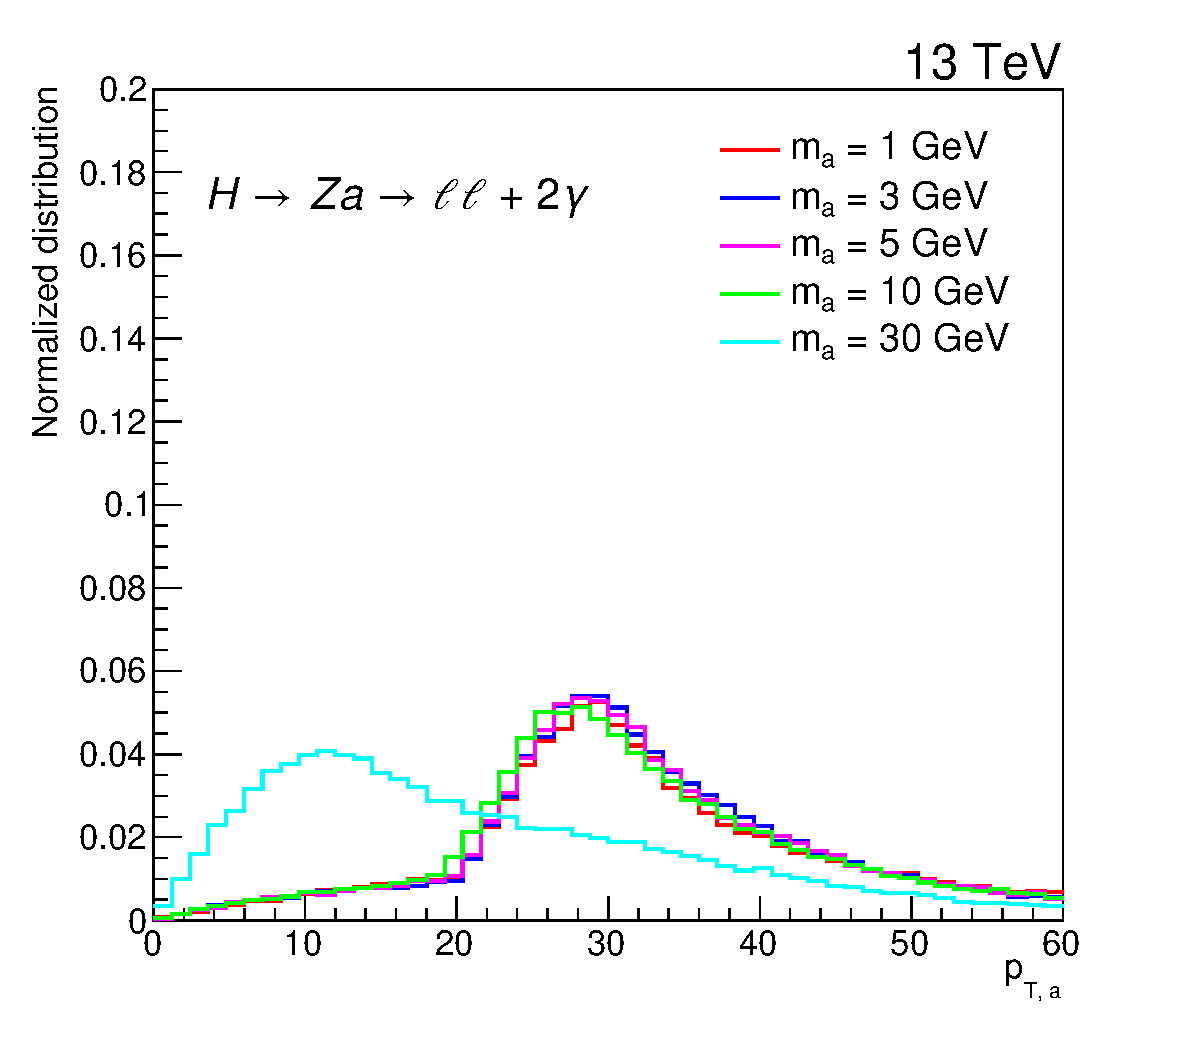
\includegraphics[width=0.45\textwidth]{Thesis (Version 2246)/figures/chapter04/ALP_pt.pdf}    
    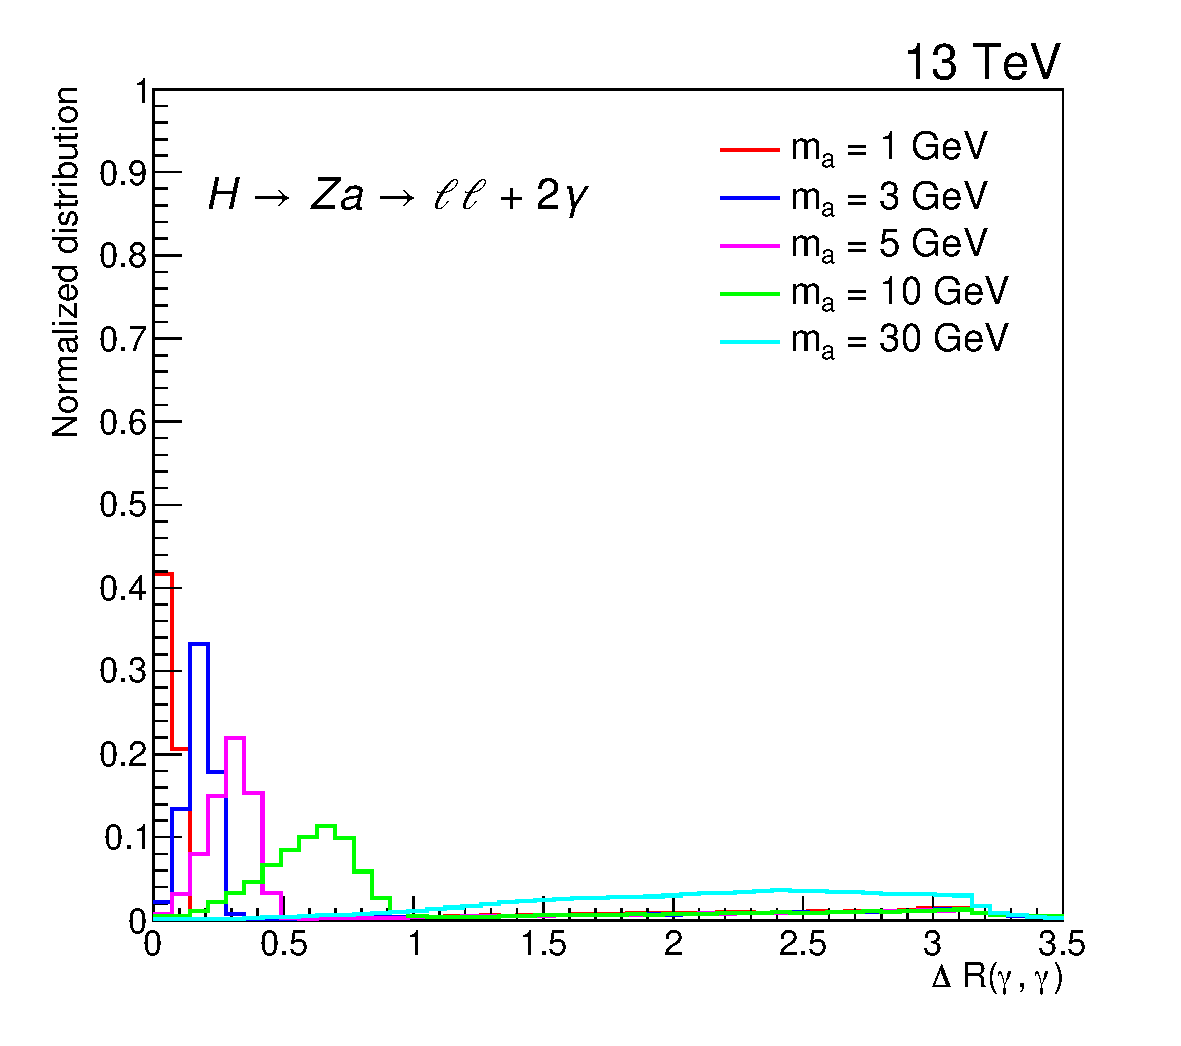
\includegraphics[width=0.45\textwidth]{Thesis (Version 2246)/figures/chapter04/dR_gg.pdf} \\
    \bicaption{\quad \centering 左图:不同ALPs质量点重建出的ALPs的横动量分布。右图:不同ALPs质量点的$\dR(\gamma,\gamma)$分布。所有的分布都被归一化}{\quad \centering Left: Reconstructed ALPs $\pt$ distributions for different ALPs mass points. Right: $\dR(\gamma,\gamma)$ distributions for different ALPs mass points. All of these distributions have been normalized}
    \label{fig:dR_pt}
\end{center}
\end{figure}

但是,当类轴子的质量比较小的时候,由Higgs衰变产生的类轴子会具有比较高的横动量,此时由类轴子衰变产生的两个光子会具有非常小的角距离,具体表现为两个光子之间的$\dR$会非常小。图~\ref{fig:dR_pt}展示了不同类轴子质量下重建出的类轴子$\pt$和由类轴子衰变产生的两个光子之间的$\dR$分布。可以发现,质量越低的类轴子倾向于具有更高的横动量,由此衰变产生的两个光子具有更小的$\dR$。对于质量小于5$\GeV$的类轴子来说,衰变产生的两个光子的$\dR<0.3$,而用于辨别真假光子的tight cut-based ID中使用了光子隔离度变量$I_{\gamma}$,这个变量的计算利用了光子周围半径$\dR=0.3$的锥形体内的所有PF光子,这就意味着质量小于5$\GeV$的类轴子衰变产生的两个光子会在半径$\dR=0.3$的锥形体内部分重叠,使得计算出来的光子隔离度偏大进而将信号事例辨别为本底事例;除此之外,相距很近的两个光子也会对$\sigma_{i\eta i\eta}$的计算产生影响,使得信号事例的$\sigma_{i\eta i\eta}$结果偏大而将信号事例辨别为本底事例。图~\ref{fig:sigma_Iso}展示了不同ALPs质量点衰变产生的光子在桶部和端盖区域的$I_{\gamma}$和$\sigma_{i\eta i\eta}$分布。考虑到以上原因,为了在低质量区域内保留足够的信号选择效率,我们最终决定使用新设计的光子辨别ID,去除对信号选择效率影响比较大的$I_{\gamma}$和$\sigma_{i\eta i\eta}$作为本分析的光子辨别ID。图~\ref{fig:IDCorr_eff}展示了对于不同类轴子质量点官方cut-based photon ID和新设计的光子辨别ID之间的信号效率对比图,可以发现去除$I_{\gamma}$和$\sigma_{i\eta i\eta}$这两个变量可以在类轴子的低质量区域内将信号的选择效率恢复到和高质量区域相同的水平。但是,去除这两个变量的同时会导致本底假光子事例的增加。为此,本分析采取了参数化的决策树法(Parameterized BDTs),将$I_{\gamma}$和$\sigma_{i\eta i\eta}$这两个变量连同其他动力学变量一起作为BDTs的输入进而进一步的对本底事例进行区分,详细步骤会在第~\ref{sec:BDT}节进行介绍。

\begin{figure}[htbp]
  \begin{center}
	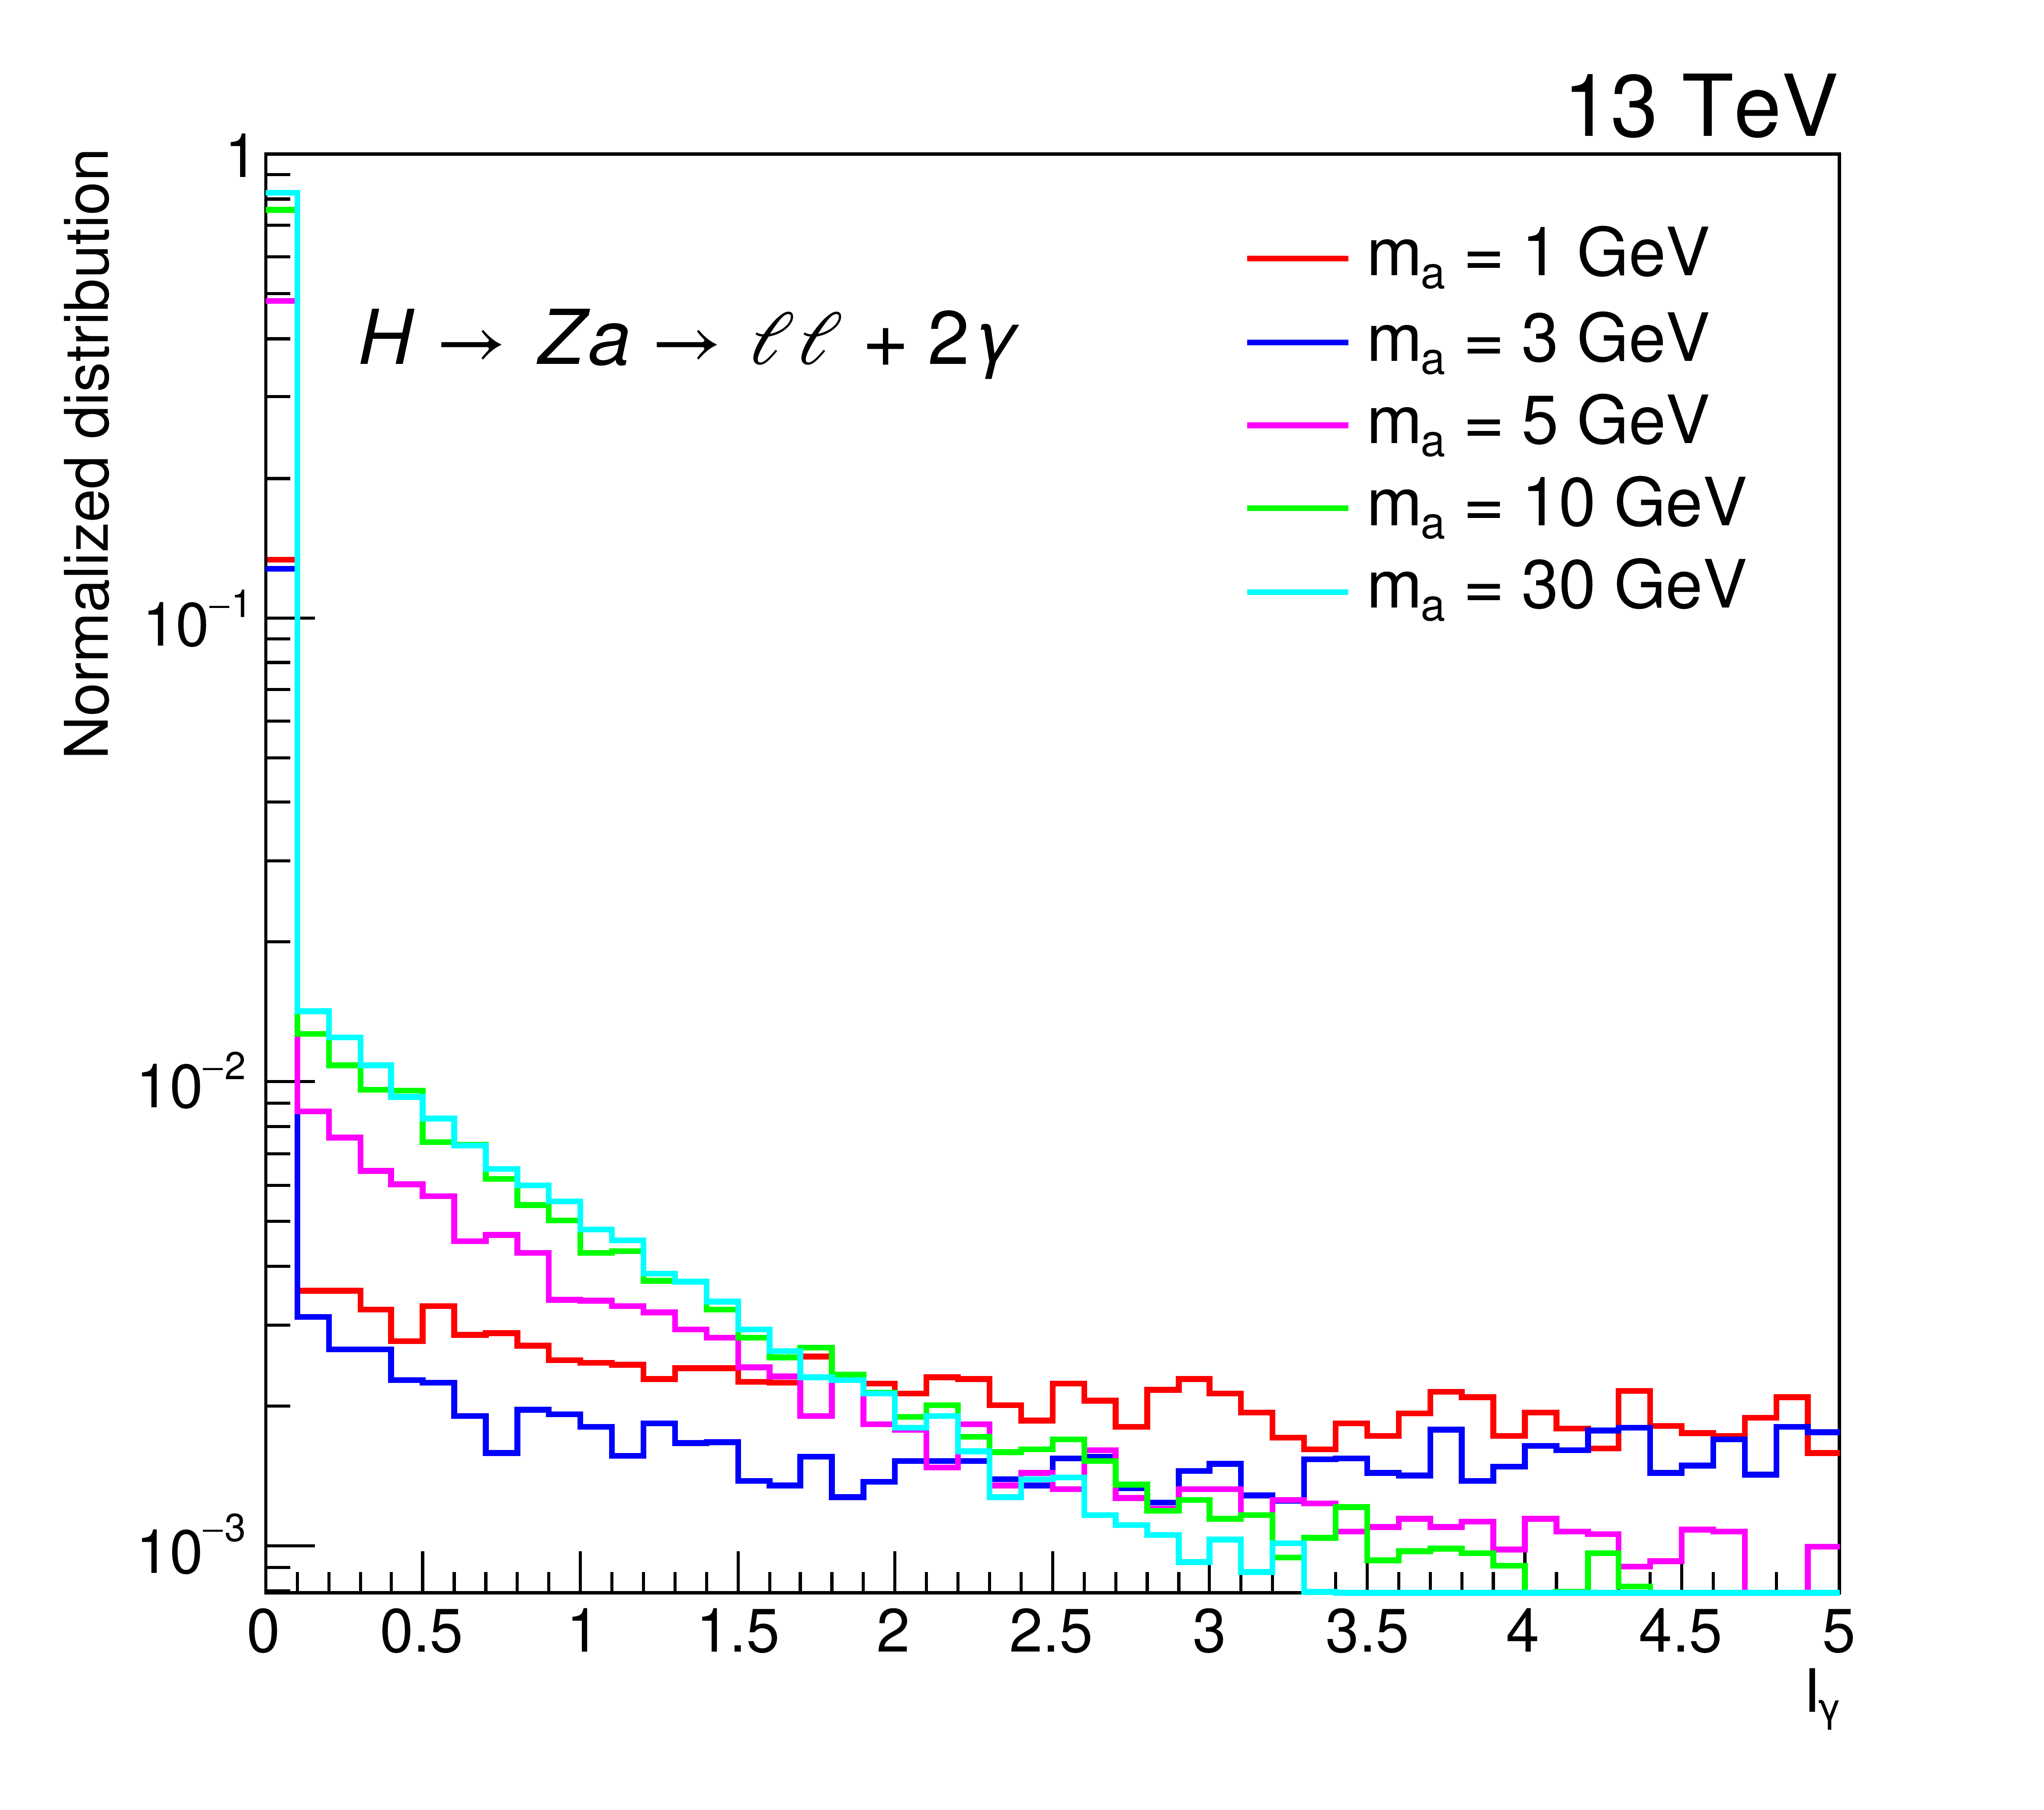
\includegraphics[width=0.45\textwidth]{figures/chapter04/pho_phoIso_EB.png}
    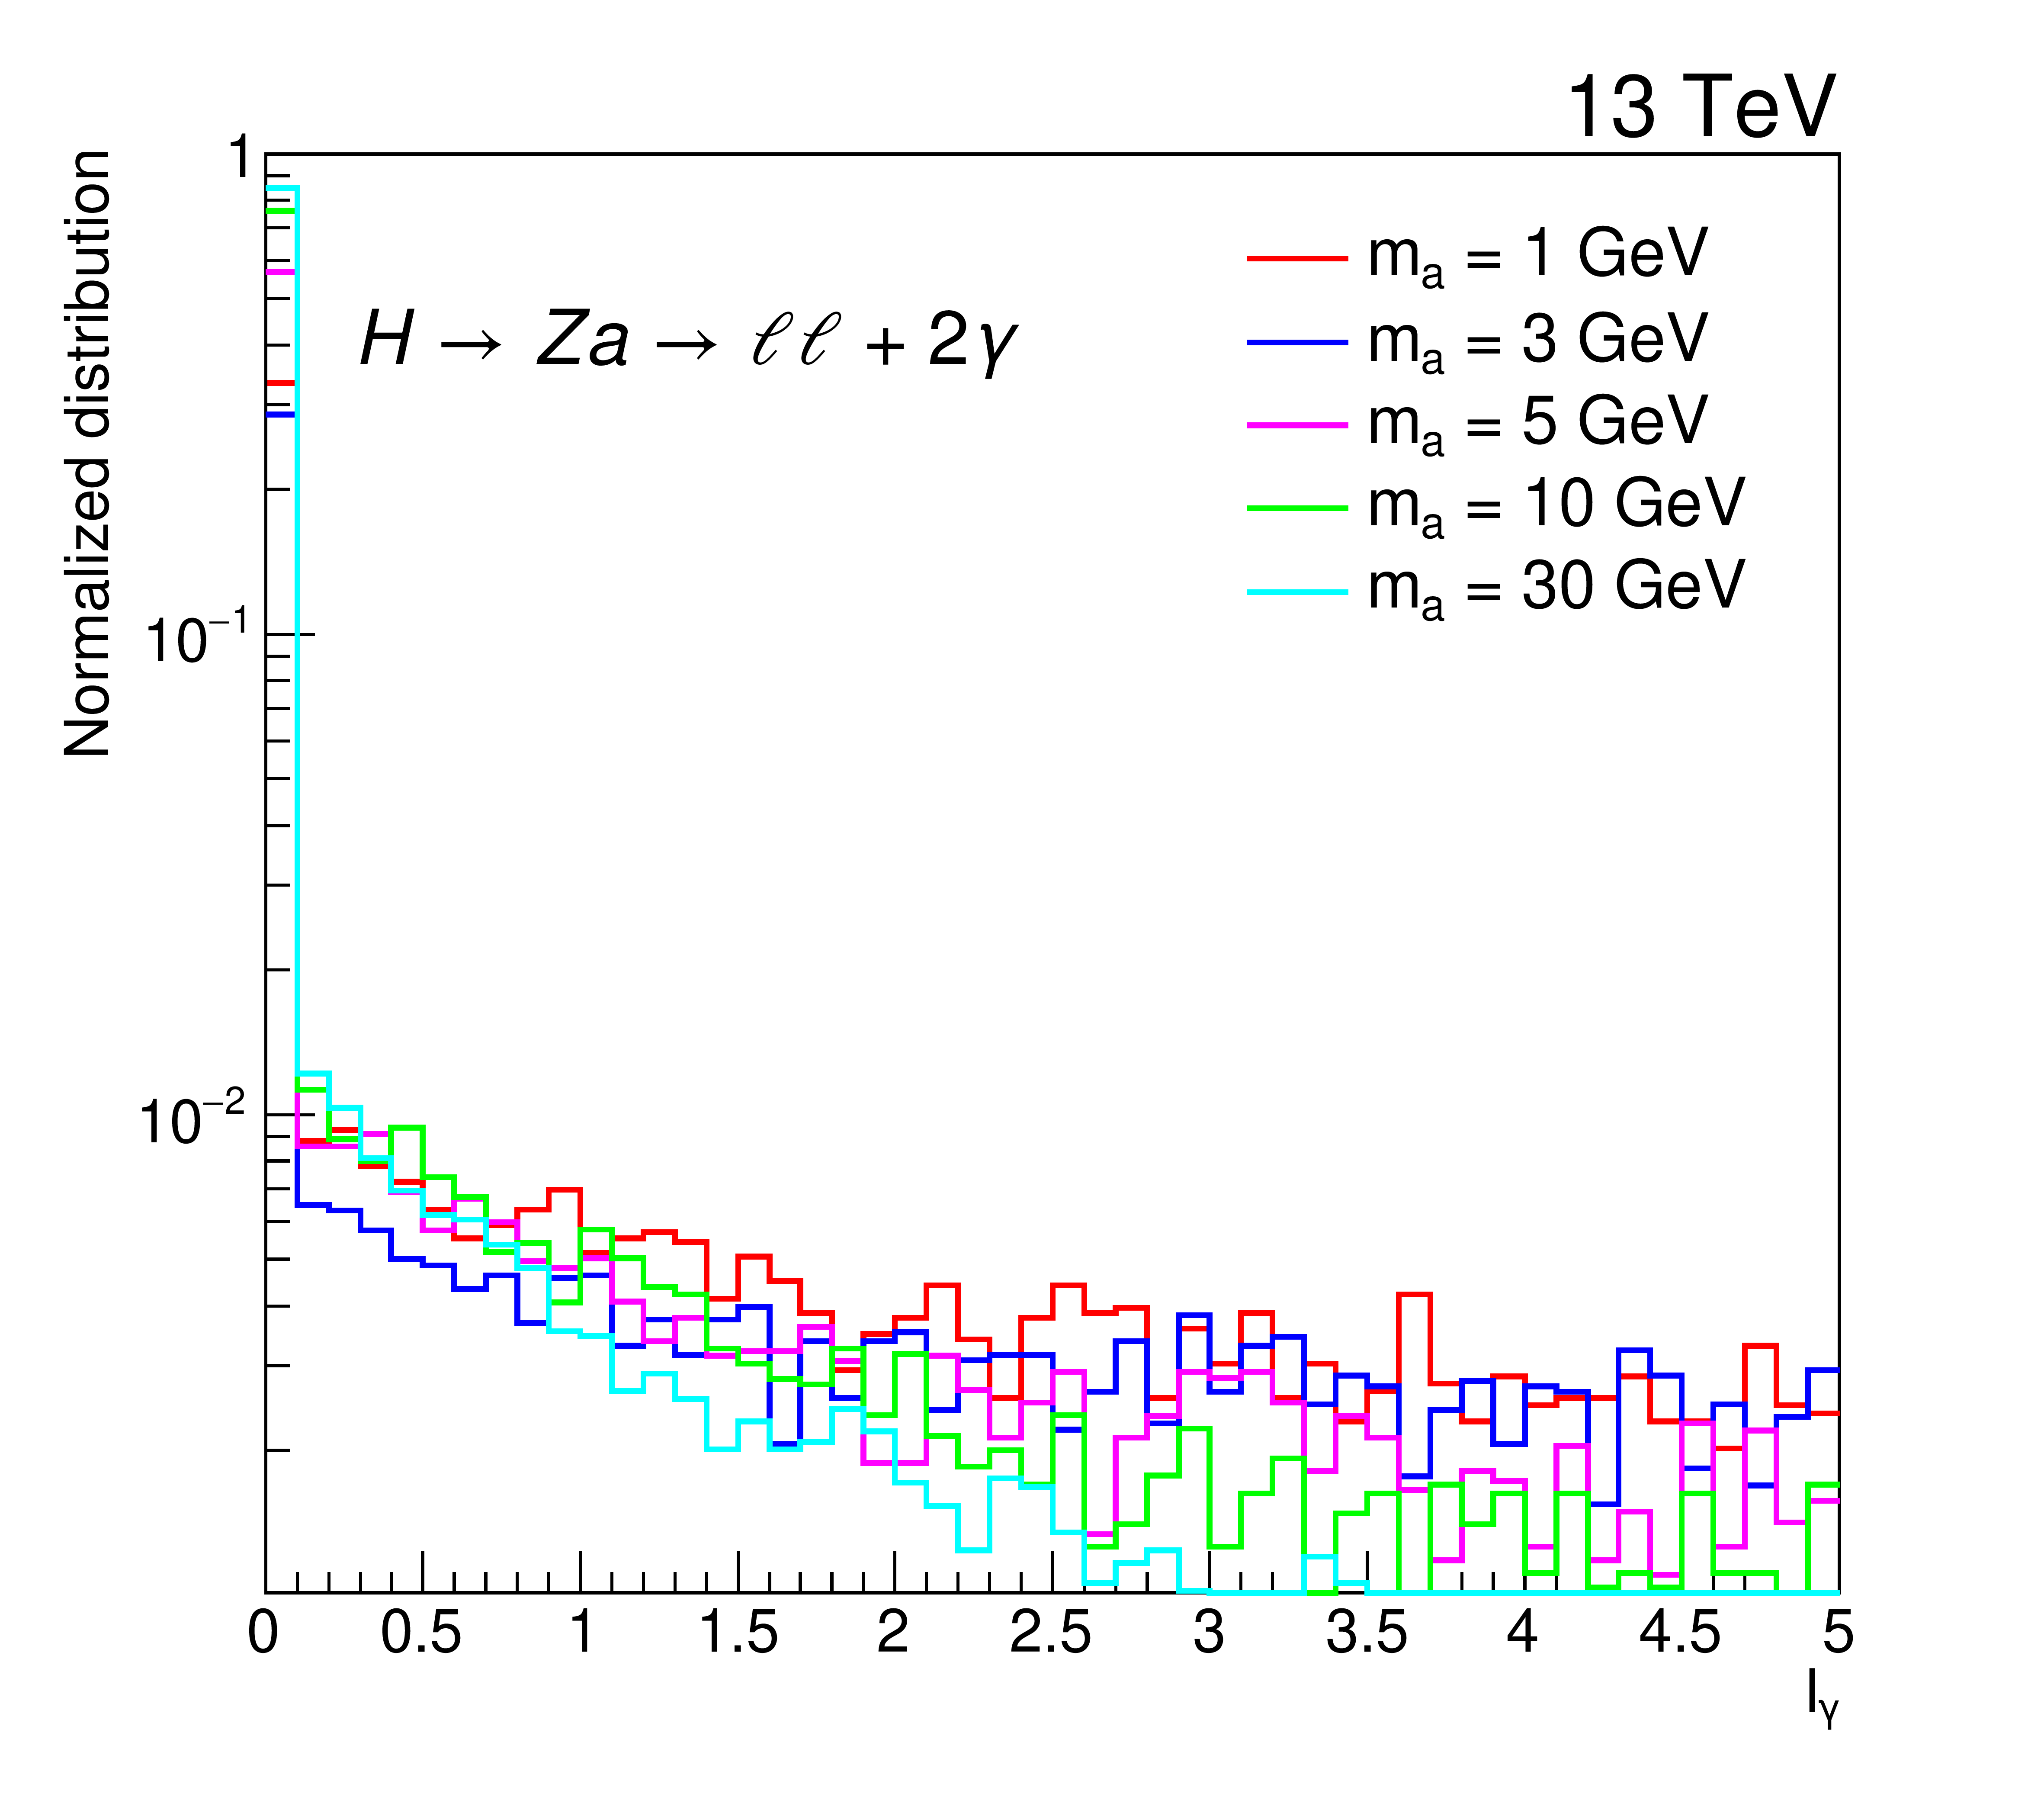
\includegraphics[width=0.45\textwidth]{figures/chapter04/pho_phoIso_EE.png} \\
    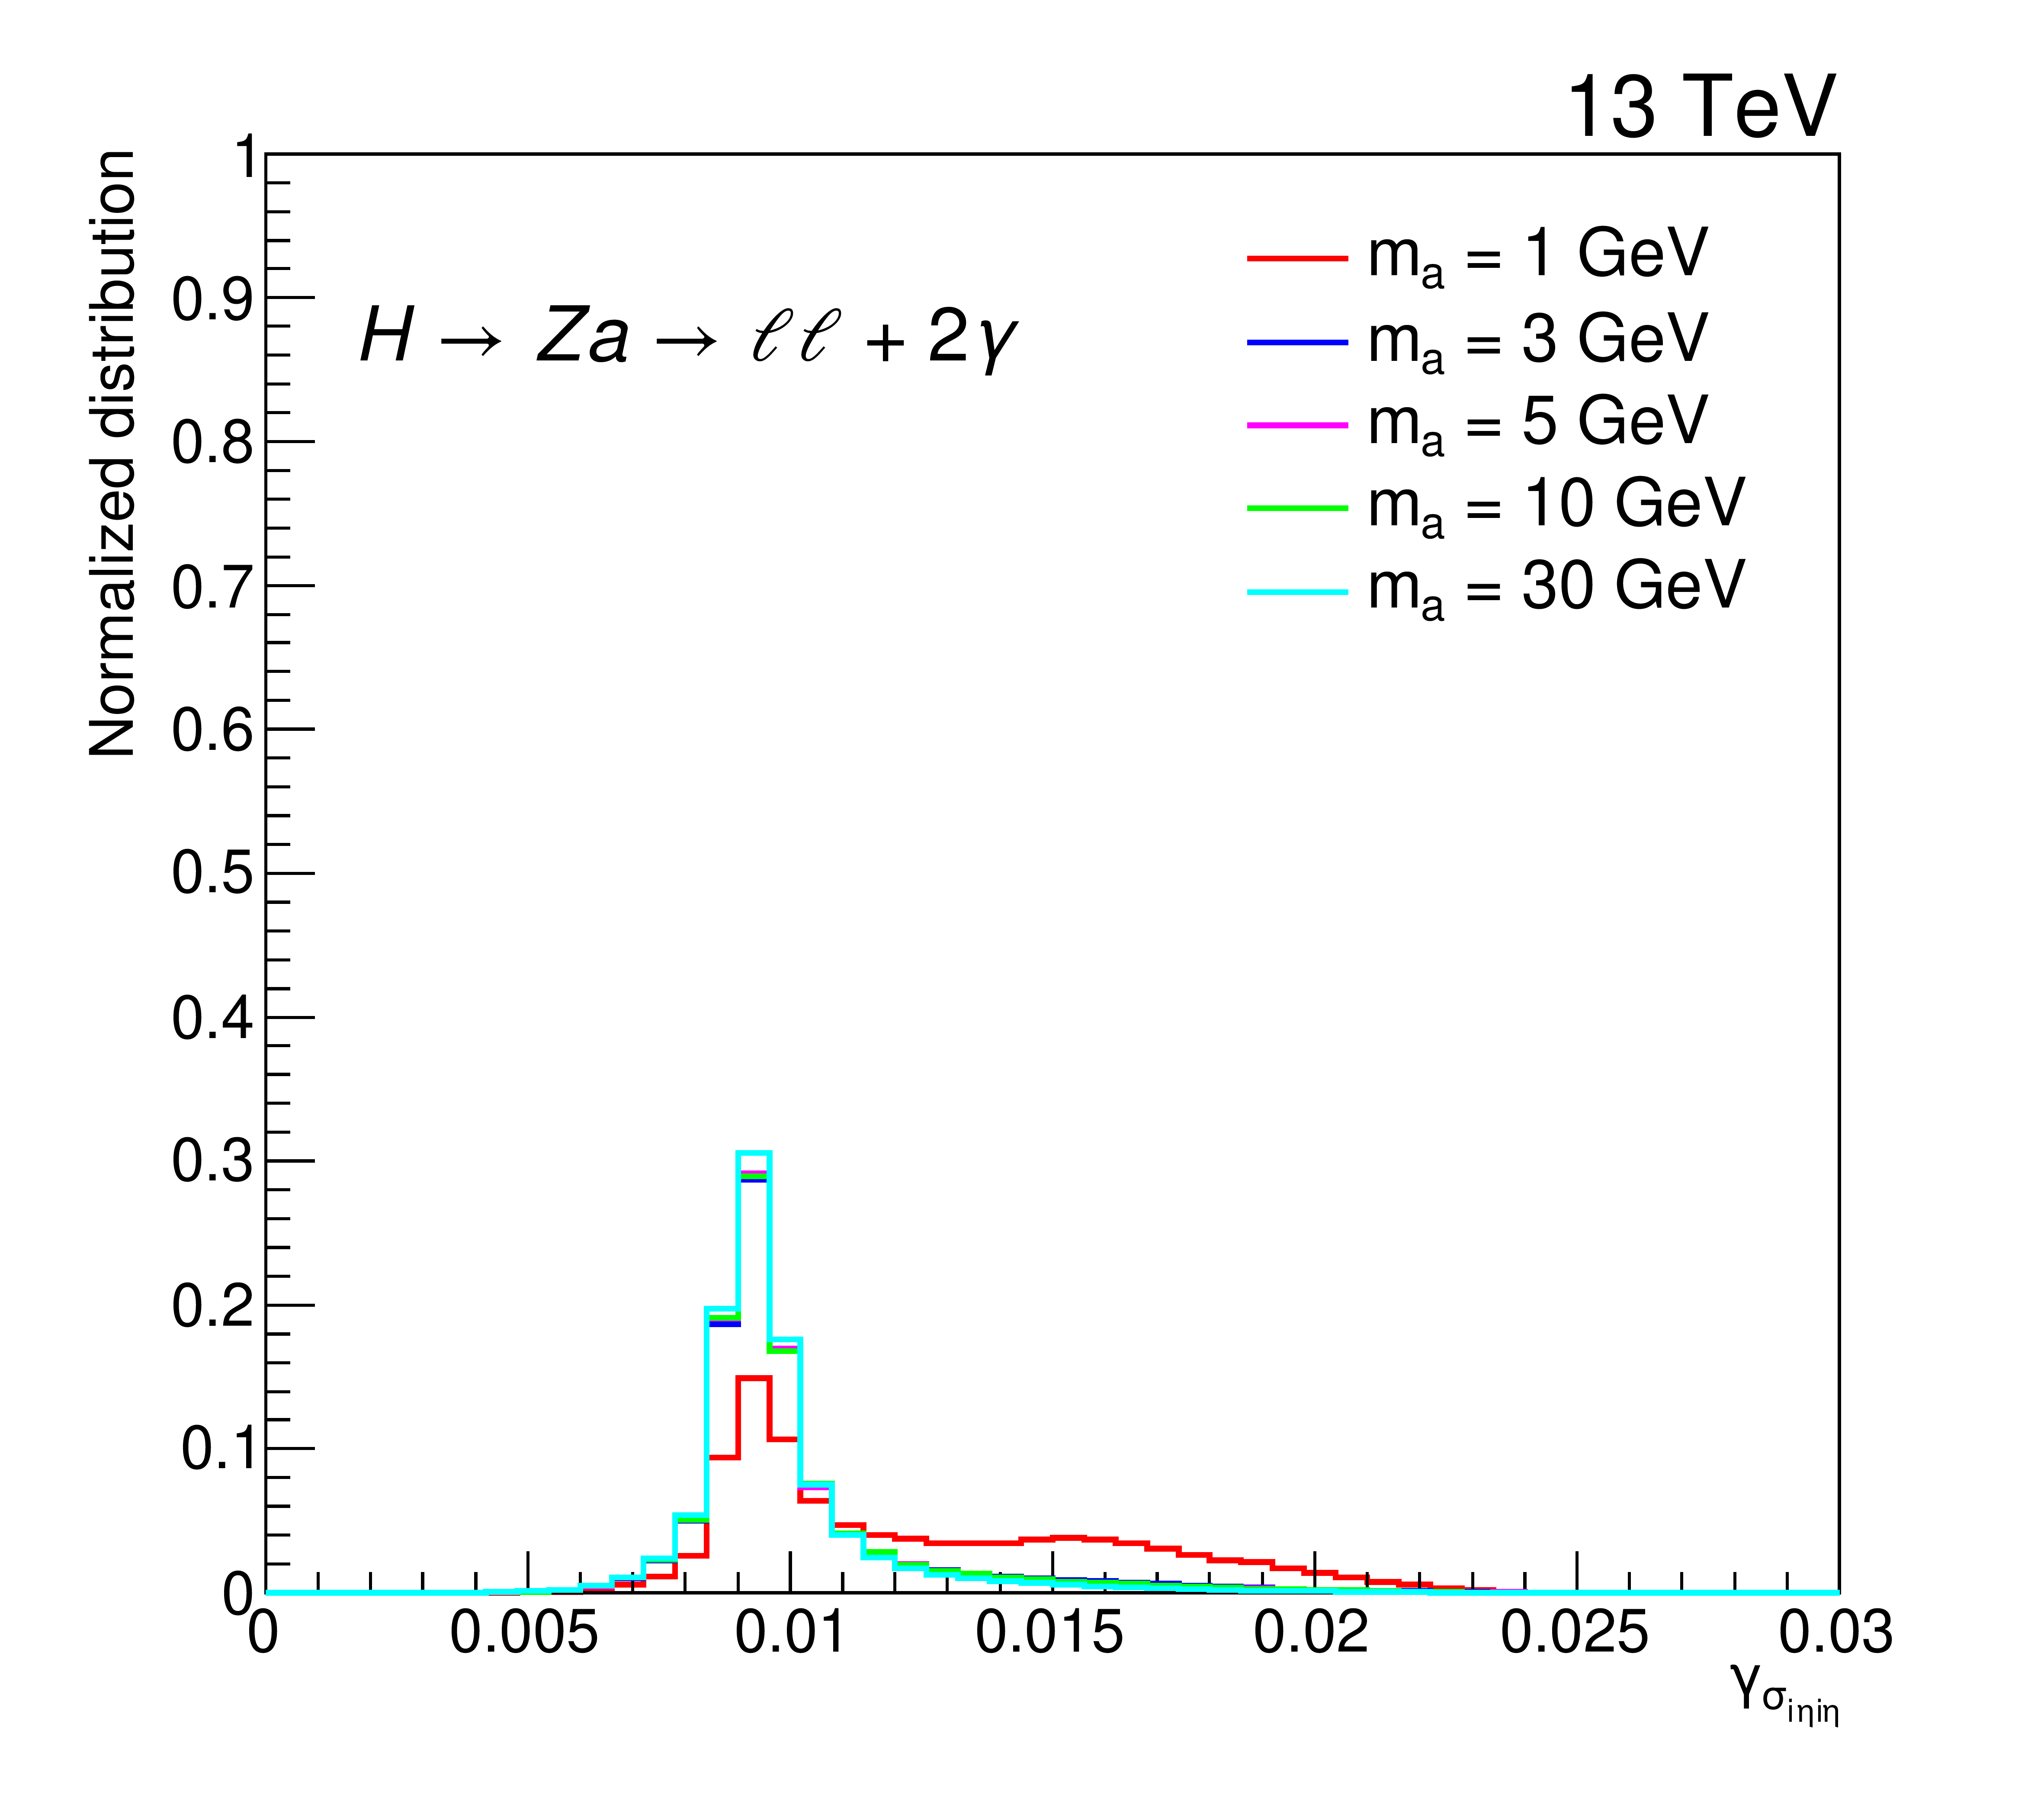
\includegraphics[width=0.45\textwidth]{figures/chapter04/pho_sigmaIetaIeta_EB.png}
    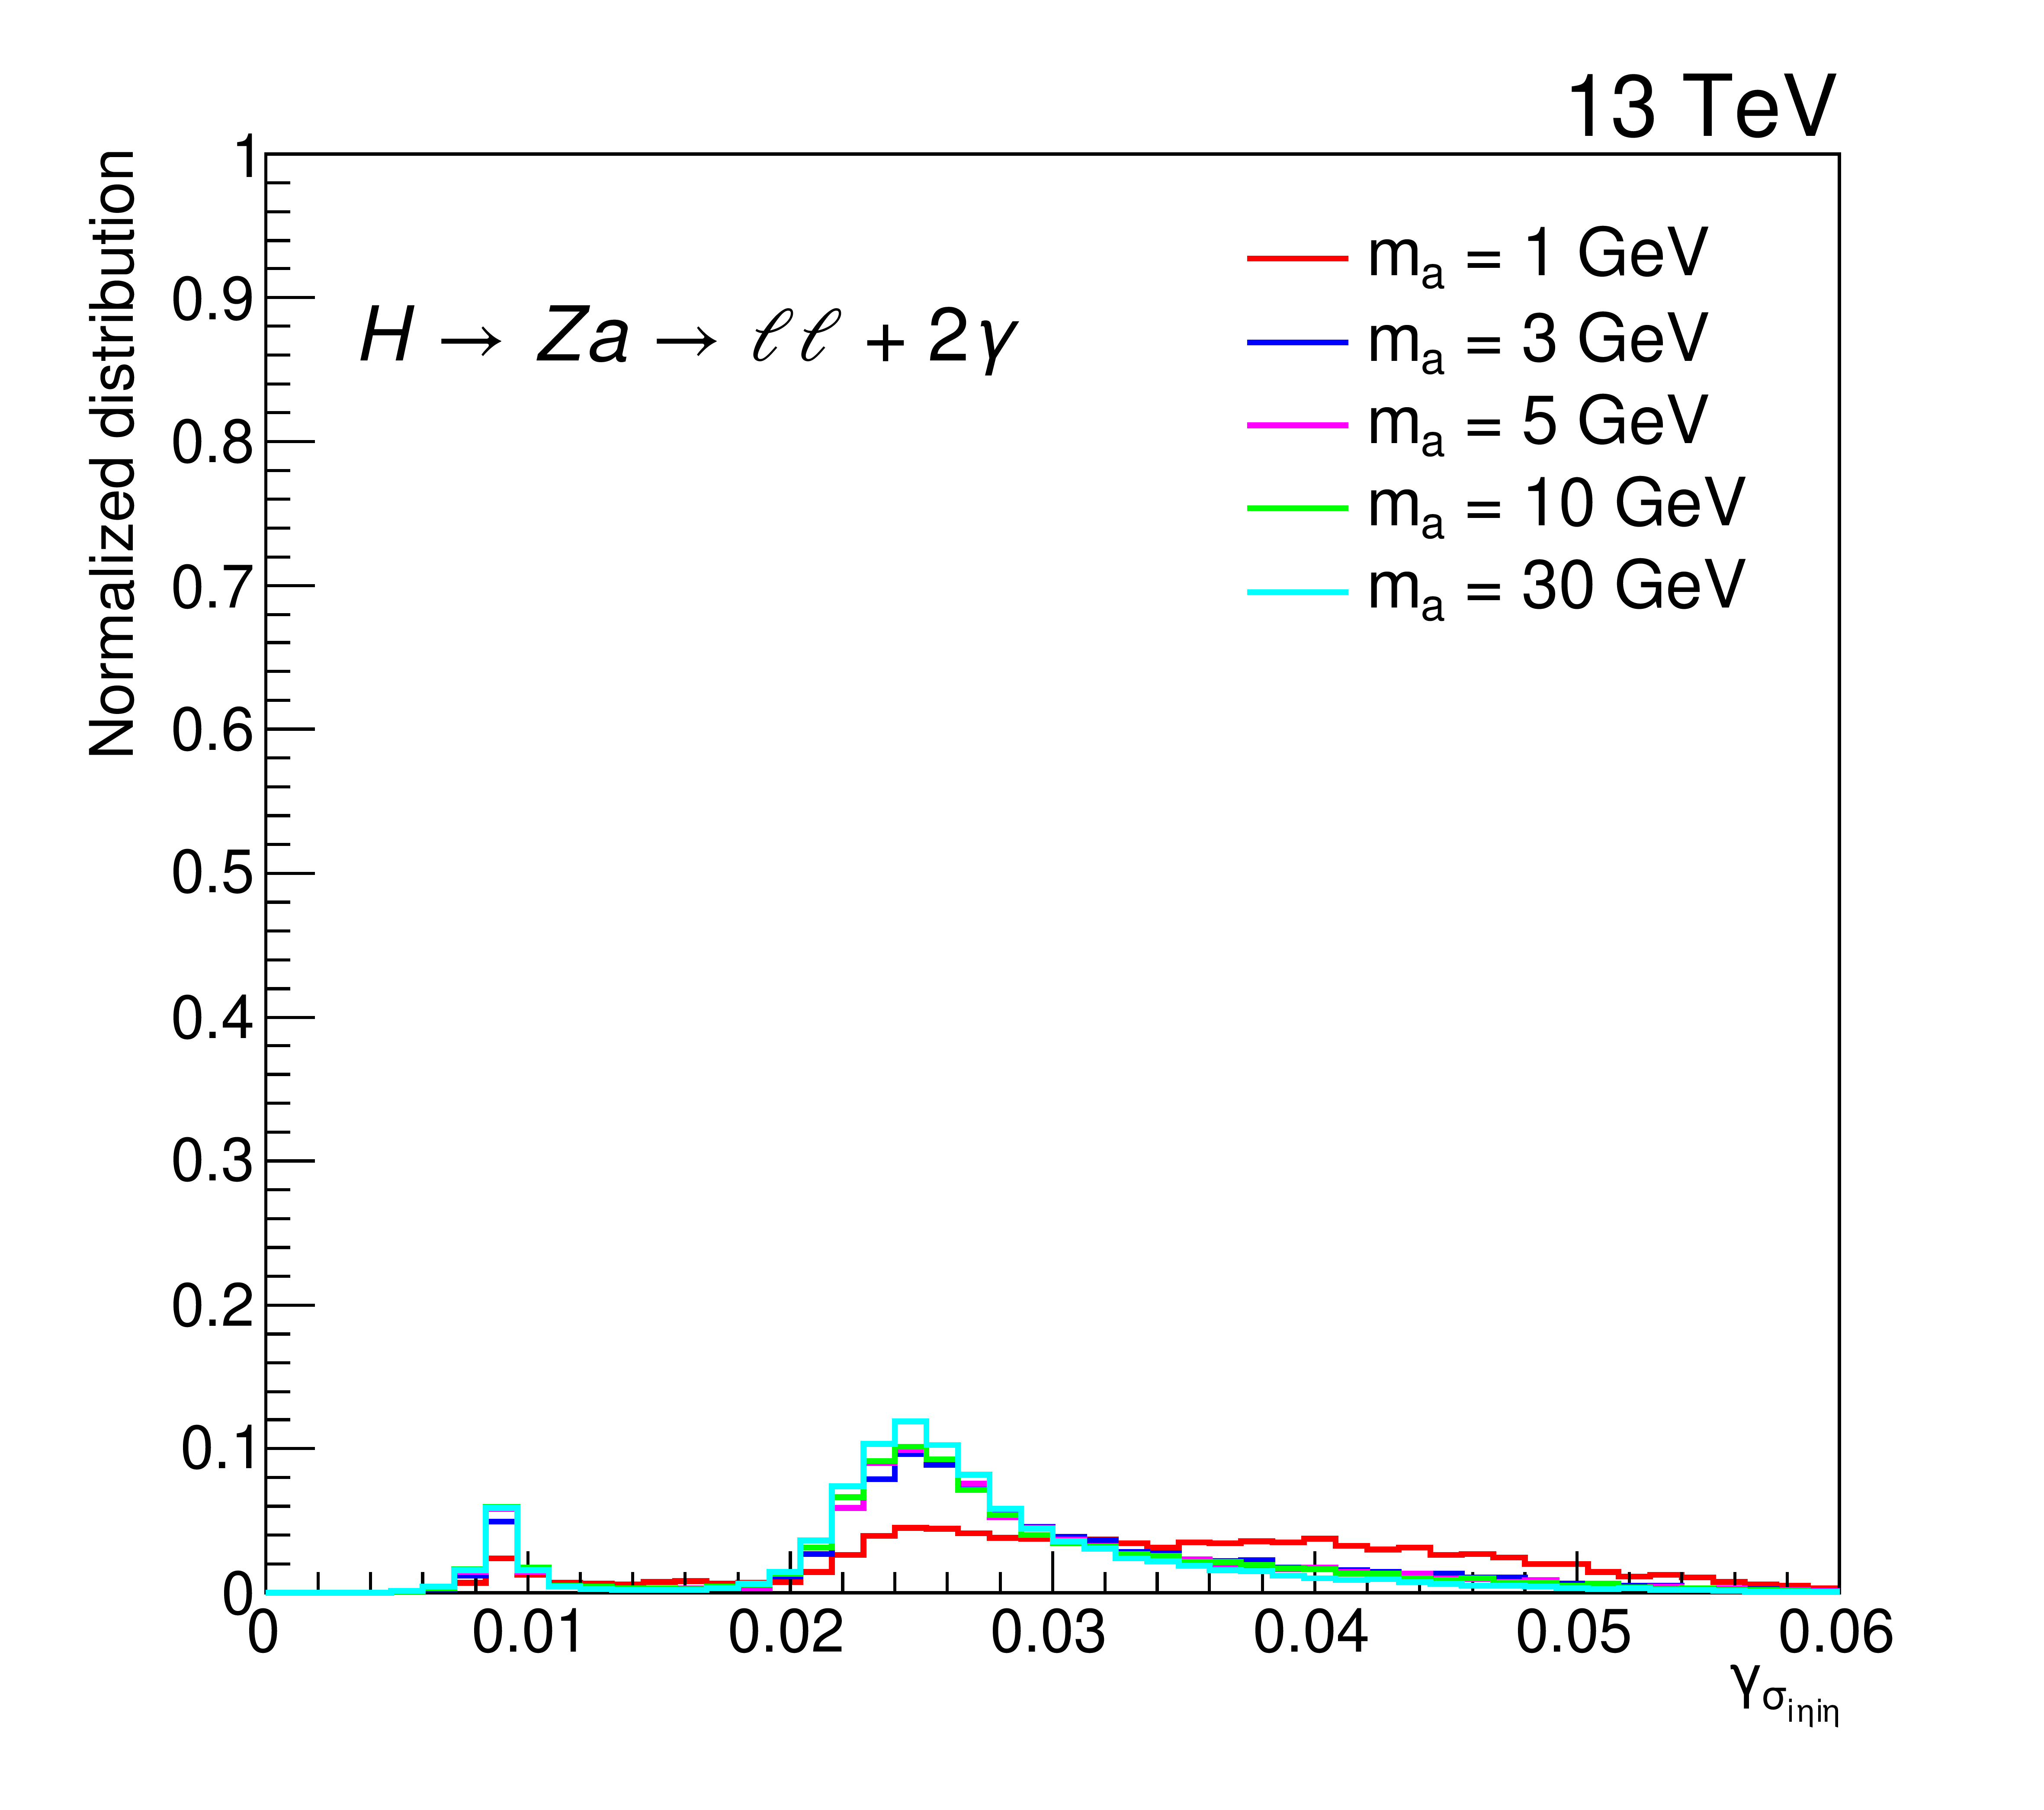
\includegraphics[width=0.45\textwidth]{figures/chapter04/pho_sigmaIetaIeta_EE.png} \\
    \bicaption{\quad \centering 上图:不同ALPs质量点的PF光子隔离度分布,左边为桶部区域,右边为端盖区域。下图:不同ALPs质量点的$\sigma_{i\eta i\eta}$分布,左边为桶部区域,右边为端盖区域。所有的分布都被归一化}{\quad \centering Top: PF photon isolation distributions for different ALPs mass points in the barrel region (left) and endcap region (right). Bottom: $\sigma_{i\eta i\eta}$ distributions for different ALPs mass points in the barrel region (left) and endcap region (right). All of these distributions have been normalized}
    \label{fig:sigma_Iso}
\end{center}
\end{figure}

\begin{figure}[htbp]
  \begin{center}
    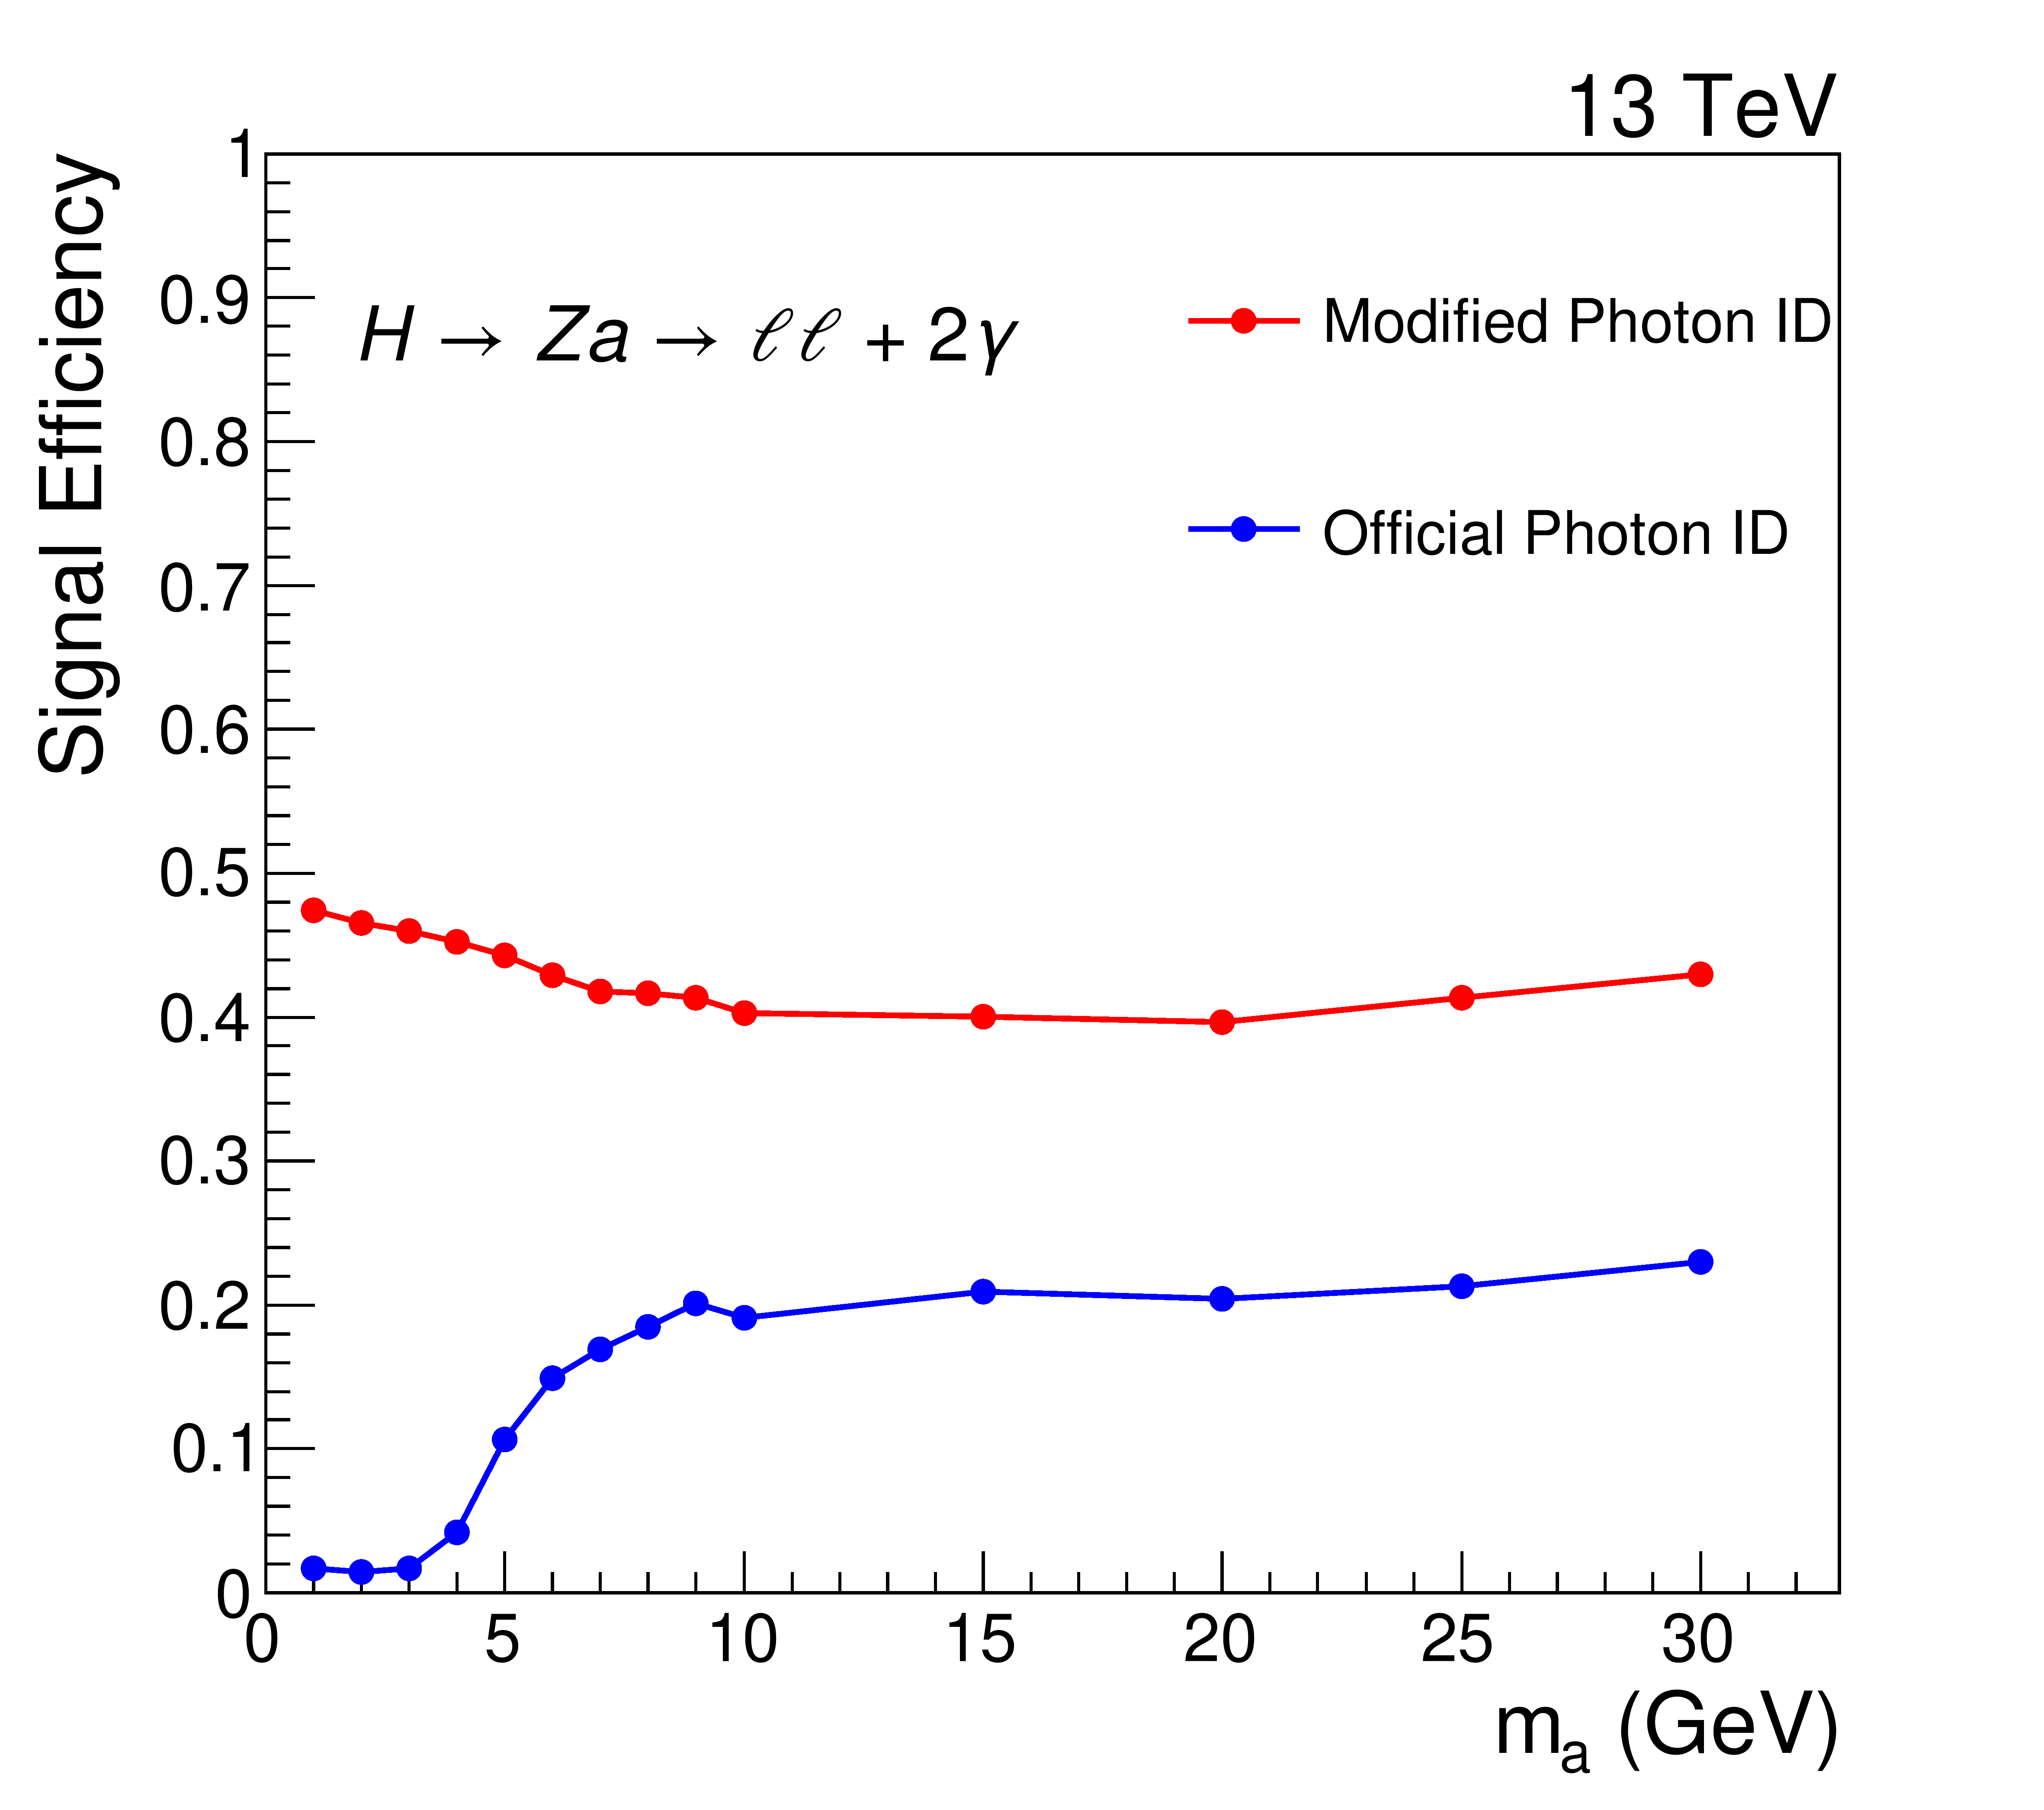
\includegraphics[width=0.45\textwidth]{figures/chapter04/ID_eff.png} \\
    \bicaption{\quad \centering 官方cut-based photon ID和新设计的ID之间信号效率的对比}{\quad \centering The comparison of signal efficiency between the official cut-based photon ID and the newly designed ID}
    \label{fig:IDCorr_eff}
\end{center}
\end{figure}


\subsection{筛选效率测量}\label{subsec:PhoTagProbe}

以上对电子、缪子和光子物理对象的筛选所造成的数据和蒙卡之间的差异可以通过利用tag-and-probe(T\&P)的方法计算出对应的比例因子(Scale Factors,SFs)来对蒙卡进行修正。T\&P方法是一种基于数据驱动(Data-driven)的技术,可以用于测量对应的探测效率。这种方法主要基于对已知的几种共振态衰变到我们所研究的特定粒子对的理解,比如$\mathrm{J/\psi}$、$\Upsilon$和Z衰变到电子对或者缪子对。

在任何物理分析中,确定探测器的效率具有至关重要的作用,它表明了对撞中产生的粒子有多少没有被探测器所接收,原因可能是来自于产生的粒子没有到达探测器探测单元或者没有被重建算法所识别等等。通常情况下,探测效率可以利用蒙卡模拟进行估算,但是由于蒙卡模拟并不完美,模拟和数据之间总是会存在微小的差异,这时就需要利用数据对蒙卡模拟进行刻度修正,T\&P方法正是一种可以直接从数据中提取效率的方法。

在这个方法中,可以利用已知的共振态衰变到特定粒子对来对探测效率进行测量。比如说可以利用$Z\rightarrow ee$的样本来对电子的选择效率进行测量,我们将衰变产生的两个电子一个定义为tag电子,另一个定义为probe电子,对它们定义的评判标准如下:

\begin{itemize}
    \item Tag电子:具有良好识别性的真电子,往往要求这个电子通过严格的筛选条件。
    \item Probe电子:没有偏差的电子候选体,往往要求这个电子通过非常宽松的筛选条件,它可以是通过或者没有通过我们将要测量的筛选条件的任何电子。
\end{itemize}
由于我们利用了特定的$Z\rightarrow ee$样本,样本中的所有事例绝大部分都是由Z衰变所产生的两个电子,tag电子的选择可以反向作为$Z\rightarrow ee$事例的触发,可以确保筛选出来的$Z\rightarrow ee$事例的纯度。而另一个probe电子的筛选是为了尽可能的保留的$Z\rightarrow ee$事例,并且可以用这个电子作为测量效率的工具。

探测效率的定义如下:
\begin{equation}
    \varepsilon = \frac{N_{pass}}{N_{total}}
\end{equation}
其中,$N_{pass}$表示通过筛选条件的probe电子的事例数,$N_{total}$指的是所有probe电子的事例数,是所有通过和未通过筛选条件的probe电子数总和。由于数据中没有办法完全排除本底,直接使用事例数所得到的探测效率往往会有较大的误差。但是由于tag-probe电子对的不变质量谱可以在Z玻色子的质量点处构成一个共振态,因此可以利用拟合数据的方法扣除本底的贡献,进而得到更为准确的探测效率。在分别得到对应数据和蒙卡之间的探测效率之后,由筛选条件所造成的数据和蒙卡之间的差异可以使用比例因子来对蒙卡样本进行修正,比例因子的定义如下:
\begin{equation}
    SFs = \frac{\varepsilon_{Data}}{\varepsilon_{MC}}
\end{equation}
其中,$\varepsilon_{Data}$指的是数据的测量效率,$\varepsilon_{MC}$指的是蒙卡的测量效率。SFs的计算往往可以分为不同的$\pt-\eta$区间,在不同的$\pt-\eta$区间内分别计算探测效率和对应的SFs可以得到更为准确的结果。

由电子的loose筛选和tight筛选所造成的数据和蒙卡样本之间的差异可以利用上述方法计算对应的SFs并将其应用到蒙卡样本的修正中解决。本分析所使用的电子loose cut比例因子由CMS实验官方提供,而电子的tight cut所对应的比例因子由CMS实验$H\rightarrow ZZ\rightarrow 4\ell$物理分析组~\cite{cmsHZZ}提供,图~\ref{fig:EleIDEff}展示了整个Run2三年的电子SFs测量结果以及对应的不确定性。

\begin{figure}[htbp]
  \begin{center}
		\includegraphics[width=0.7\textwidth,page=3]{figures/chapter04/2016_egammaEffitxt_egammaPlots.pdf}
    \includegraphics[width=0.75\textwidth,page=3]{figures/chapter04/2017_egammaEffitxt_egammaPlots.pdf} \\
		\includegraphics[width=0.7\textwidth,page=3]{figures/chapter04/2018_egammaEffitxt_egammaPlots.pdf}
    \bicaption{\quad \centering 左边:所有数据相对于模拟的电子SFs作为$\pt$和$\eta$的函数。右边:数据相对于模拟的电子SFs的不确定性作为$\pt$和$\eta$的函数。顶部显示了2016年的结果,中间显示了2017年的结果,底部显示了2018年的结果}{\quad \centering Left: Overall data to simulation scale factors for electrons, as function of $\pt$ and $\eta$. Right: Uncertainties on  data to simulation scale factors for electrons, as a function of $\pt$ and $\eta$. Results are shown for 2016 (top), 2017 (middle), and 2018 (bottom)}
    \label{fig:EleIDEff}
\end{center}
\end{figure}

利用以上方法,我们也可以对缪子的探测效率进行测量,唯一的不同就是所使用的样本是$Z\rightarrow \mu\mu$过程。而对于低$\pt$的缪子效率测量,由于$\mathrm{J/\psi}$的质量相比于Z玻色子小很多,衰变产生的两个缪子的$\pt$会比较小,因此可以利用$\mathrm{J/\psi}\rightarrow\mu\mu$的样本来对低动量区域的缪子进行效率测量。图~\ref{fig:MuonIDEff}展示了整个Run2三年的缪子SFs测量结果以及对应的不确定性。

\begin{figure}[htbp]
  \begin{center}
		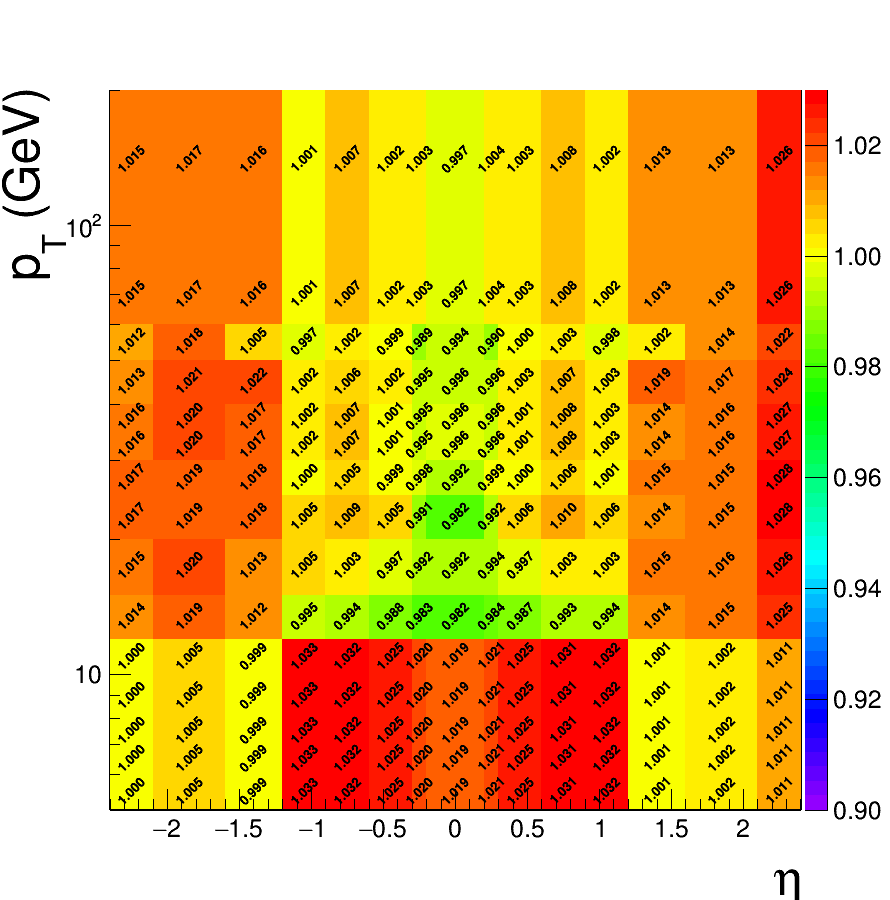
\includegraphics[width=0.45\textwidth]{figures/chapter04/2016_SF_legacy_newLoose.png}
    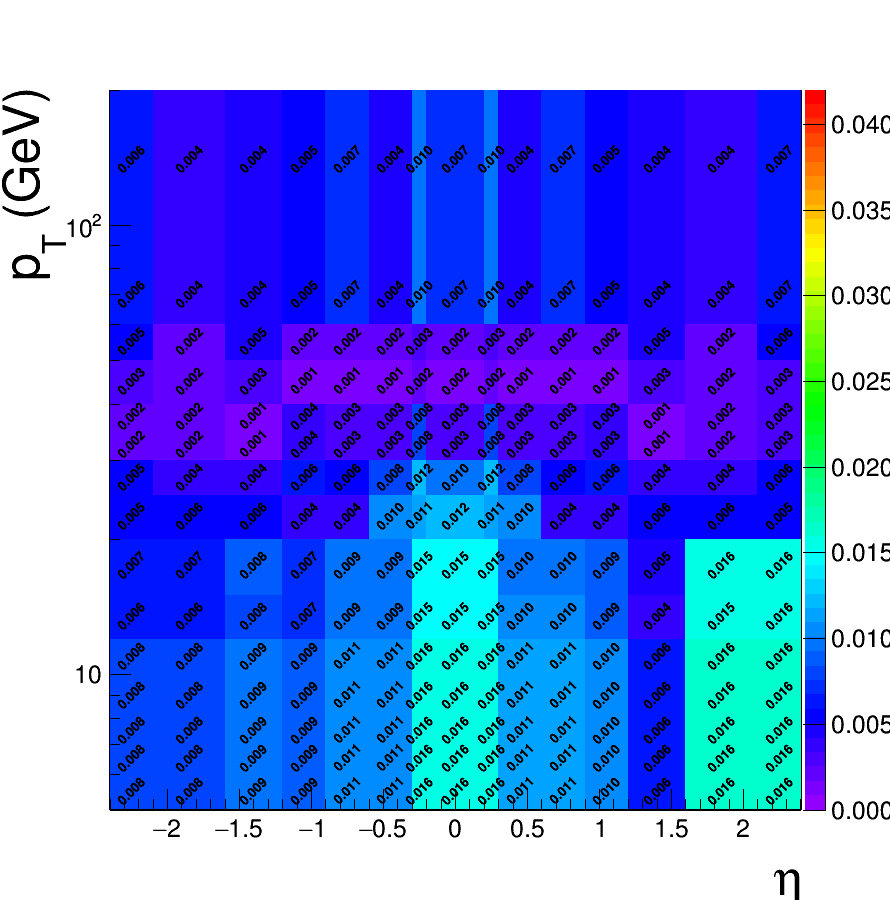
\includegraphics[width=0.45\textwidth]{figures/chapter04/2016_SF_errors_legacy_newLoose.png} \\
		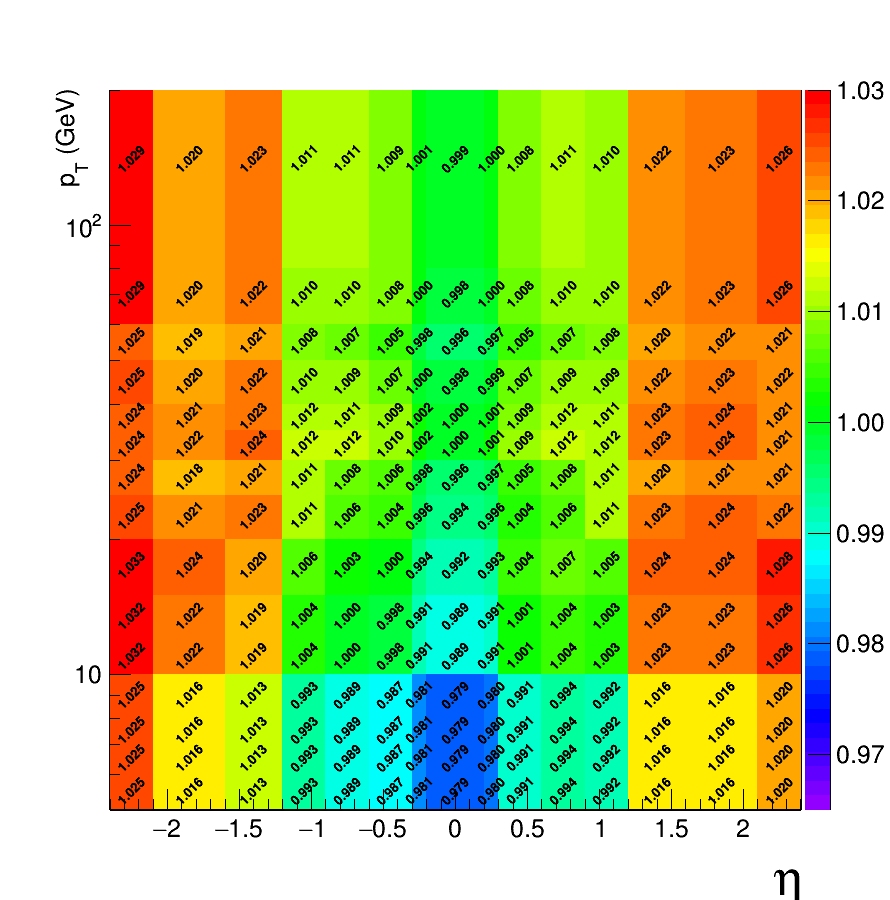
\includegraphics[width=0.45\textwidth]{figures/chapter04/2017_SF_rereco_LooseGT20syst.png}
    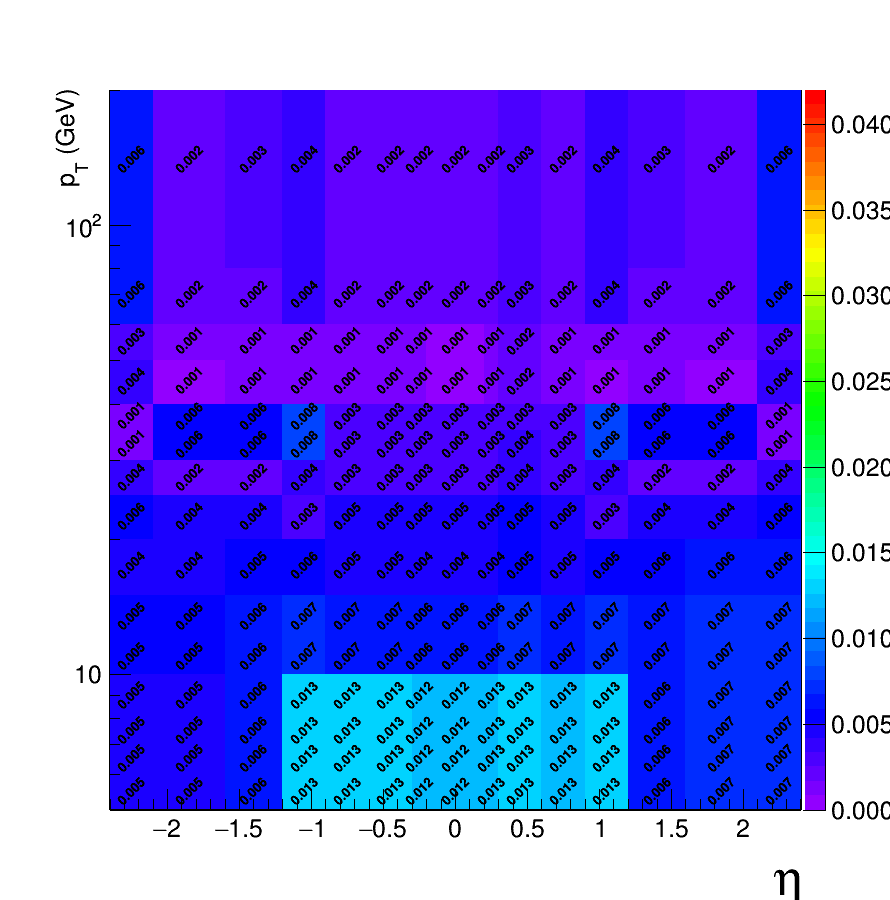
\includegraphics[width=0.45\textwidth]{figures/chapter04/2017_SF_errors_rereco_LooseGT20syst.png} \\
		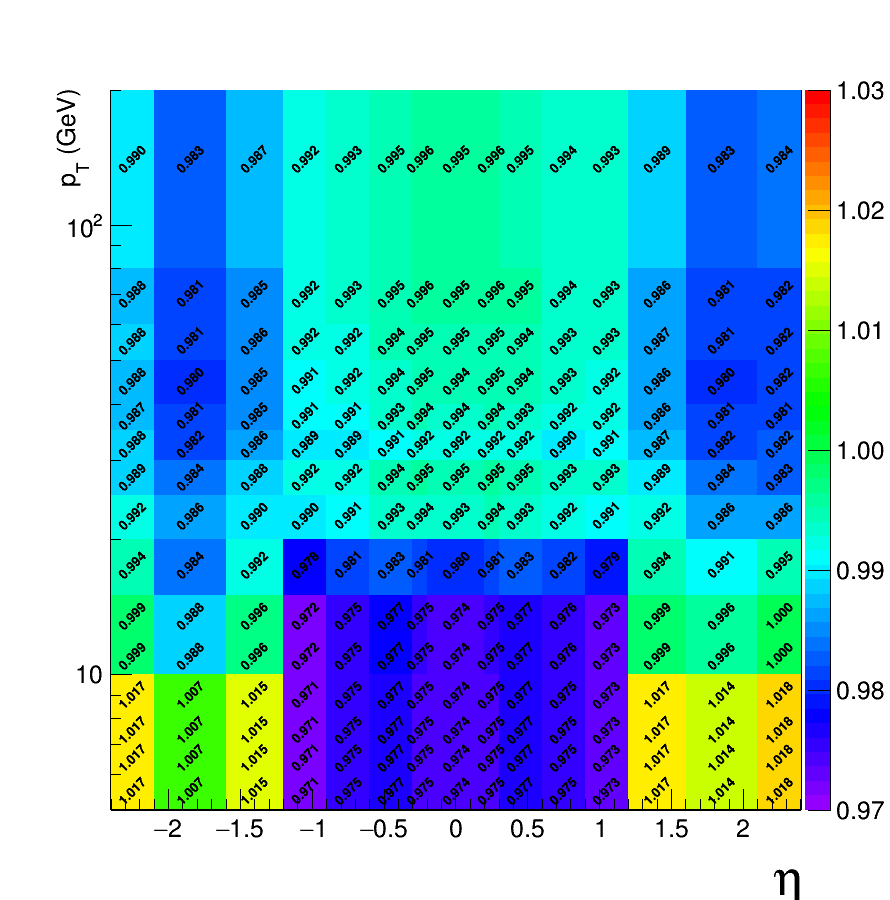
\includegraphics[width=0.45\textwidth]{figures/chapter04/2018_SF_rereco_LooseGT20syst.png} 
		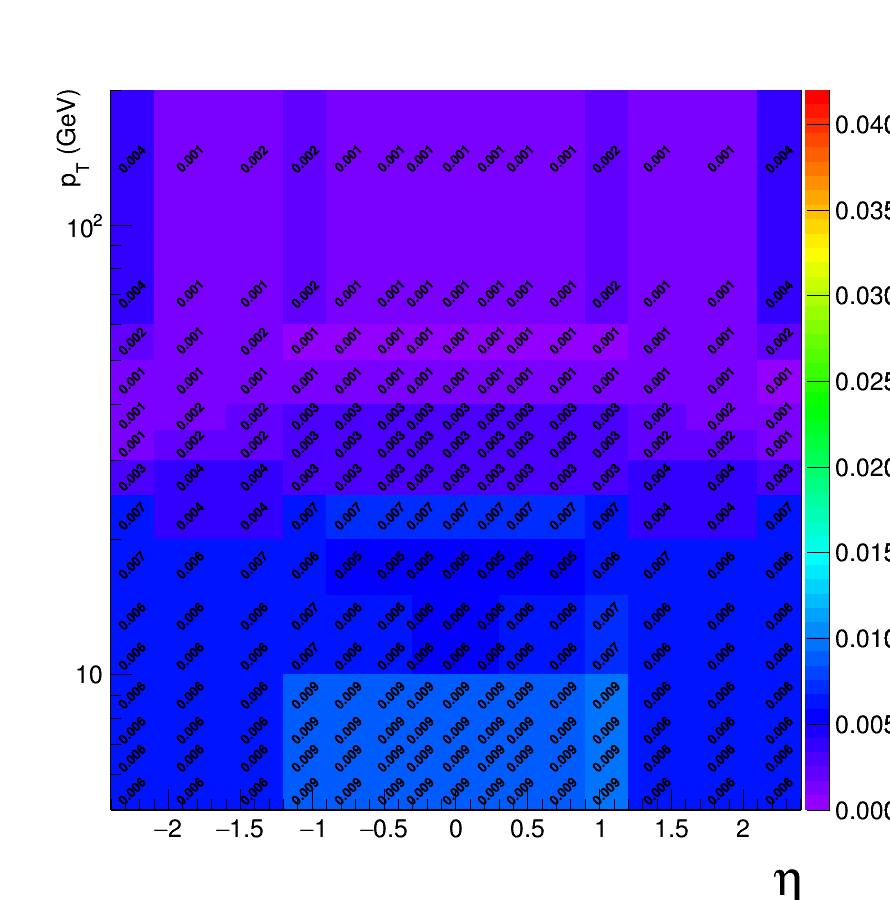
\includegraphics[width=0.45\textwidth]{figures/chapter04/2018_SF_errors_rereco_LooseGT20syst.png}
    \bicaption{\quad \centering 左边:所有数据相对于模拟的缪子SFs作为$\pt$和$\eta$的函数。右边:数据相对于模拟的缪子SFs的不确定性作为$\pt$和$\eta$的函数。顶部显示了2016年的结果,中间显示了2017年的结果,底部显示了2018年的结果}{\quad \centering Left: Overall data to simulation scale factors for muons, as function of $\pt$ and $\eta$. Right: Uncertainties on  data to simulation scale factors for muons, as a function of $\pt$ and $\eta$. Results are shown for 2016 (top), 2017 (middle), and 2018 (bottom)}
    \label{fig:MuonIDEff}
\end{center}
\end{figure}

而对于光子效率的测量,由于在CMS探测器中电子和光子的重建过程几乎完全相同,唯一的区别就是电子会在中心径迹室留下轨迹。因此,我们仍然可以利用$Z\rightarrow ee$的事例来对光子进行效率测量,唯一的区别就是我们使用的是由电子所假扮的假光子。为了满足这一要求,我们只需将由中心径迹室所决定的conversion-safe electron veto这一要求应用到电子上,就可以得到用于光子测量的假光子。

\begin{table}[h]
    \centering
    \bicaption{\quad \centering 用于测量光子效率所使用的样本}{\quad \centering Samples used for photon efficiencies measurement}
    \resizebox{\textwidth}{!}{
    \begin{tabular}{ll} \hline
        Datasets & File name \\ \hline
       2016 pre-VFP & [1]UL2016\_SingleEle\_Run2016[B,C,D,E,F].root \\ 
        & [1]DYJetsToLL\_M-50\_TuneCP5\_13TeV-madgraphMLM-pythia8\_preVFP\_UL2016.root \\ 
        & [1]DYJetsToLL\_M-50\_TuneCP5\_13TeV-amcatnloFXFX-pythia8\_preVFP\_UL2016.root \\ \hline
       2016 post-VFP & [2]UL2016\_SingleEle\_Run2016[F\_postVFP, G, H] \\ 
      & [2]DYJetsToLL\_M-50\_TuneCP5\_13TeV-madgraphMLM-pythia8\_postVFP\_UL2016.root \\ 
      & [2]DYJetsToLL\_M-50\_TuneCP5\_13TeV-amcatnloFXFX-pythia8\_postVFP\_UL2016.root \\ \hline
      2017 & [3]SingleEle\_Run[B,C,D,E,F].root \\
        & [3]DYJetsToEE.root \\ 
        & [3]DYJetsToLL\_amcatnloFXFX.root\\ \hline
        2018 & [4]EGamma\_Run[A,B,C,D].root \\ 
        & [4]DYJetsToLL\_madgraphMLM.root \\ 
        & [4]DYJetsToLL\_amcatnloFXFX.root \\ \hline
       \multicolumn{2}{l}{[1] = /eos/cms/store/group/phys\_egamma/akapoor/Tag-and-Probe\_Tree/UL2016\_ntuples/}\\
       \multicolumn{2}{l}{[2] = /eos/cms/store/group/phys\_egamma/akapoor/Tag-and-Probe\_Tree/UL2016\_ntuples/}\\
       \multicolumn{2}{l}{[3] = /eos/cms/store/group/phys\_egamma/asroy/Tag-and-Probe\_Tree/UL2017\_MINIAOD\_Nm1/}\\
       \multicolumn{2}{l}{[4] = /eos/cms/store/group/phys\_egamma/asroy/Tag-and-Probe\_Tree/UL2018\_MINIAOD\_Nm1/}
    \end{tabular}}
    \label{tab:TnP_datasets}
\end{table}

列表~\ref{tab:TnP_datasets}展示了本分析中光子效率测量所使用的样本,事例中的所有电子都通过conversion-safe electron veto这一要求。本分析中对新设计的光子ID效率的测量所使用的tag和probe电子的选择如下:
\begin{itemize}
    \item Tag电子:通过tight工作点,$\pt>35\GeV$并且$|\eta|<2.17$;
    \item Probe电子:$\pt>10\GeV$;
    \item 两个电子的不变质量位于60$\GeV$和120$\GeV$之间;
\end{itemize}
通过利用信号加本底的模型对双轻子的不变质量谱进行拟合可以得到对应的筛选效率。其中,拟合中的信号模型使用的是蒙卡样本中的信号模型和一个高斯函数的卷积,高斯函数主要是为了考虑探测器分辨率的影响;本底信号模型使用的是误差函数和指数函数的卷积。通过对拟合中的信号部分进行积分求和可以得到通过和未通过新设计的光子ID的事例数,从而可以得到数据和蒙卡的效率,它们之间的比值就作为蒙卡修正所使用的SFs。在本分析中,效率和SFs的测量是在以下$\pt$和$\eta$的范围中计算的:
\begin{itemize}
    \item $\pt$:10$\GeV$,15$\GeV$,20$\GeV$,35$\GeV$,50$\GeV$;
    \item $|\eta|$:0.0,0.8,1.4442,1.566,2.0,2.5;
\end{itemize}

图~\ref{fig:IDCorr_eff_fit}展示了2018年数据中效率测量的一个拟合结果,这个结果是在$-2.5<\eta<2.0$ 和 $10<\pt<15$~\si{GeV}的范围内进行测量的。其中,passing probe表示的是通过新设计的光子ID的tag-probe电子对不变质量分布图,failing probe表示没有通过的tag-probe电子对不变质量分布图。黑色的点表示数据,蓝色和红色的曲线分别表示拟合得到的本底模型和信号模型。通过对红色曲线下的面积求和就可以得到对应的通过和未通过的probe电子事例数,进而可以得到对应的效率值。然后再利用数据和蒙卡之间的效率值之比就可以得到对应区间的SFs。

\begin{figure}[htbp]
  \begin{center}
    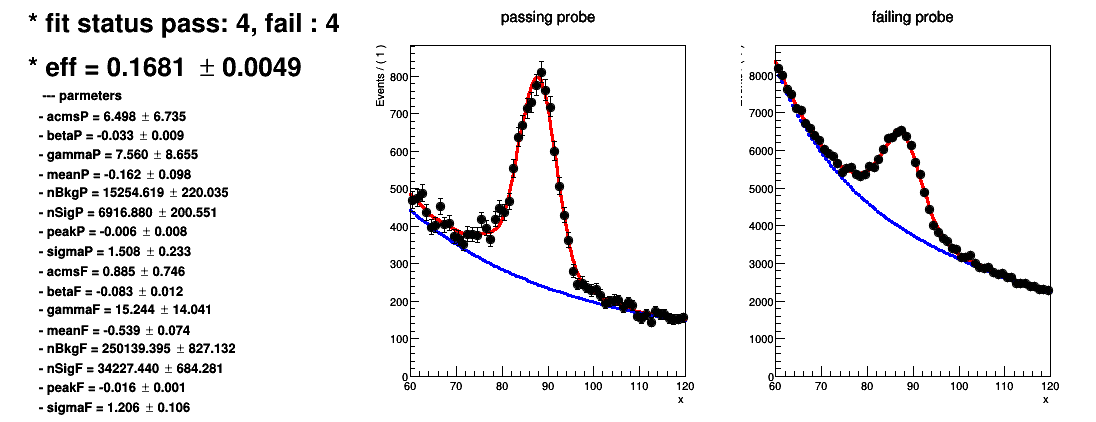
\includegraphics[width=1.0\textwidth]{figures/chapter04/bin00_ph_sc_eta_m2p50Tom2p00_ph_et_10p00To15p00.png}
    \bicaption{\quad \centering 2018年数据中效率测量在$-2.5<\eta<2.0$ \&\& $10<\pt<15$~\si{GeV}范围内的拟合结果}{\quad \centering The fitting results of the efficiency measurement in 2018 data within the bins of $-2.5<\eta<2.0$ \&\& $10<\pt<15$~\si{GeV}}
    \label{fig:IDCorr_eff_fit}
\end{center}
\end{figure}

\begin{figure}[htbp]
  \begin{center}
		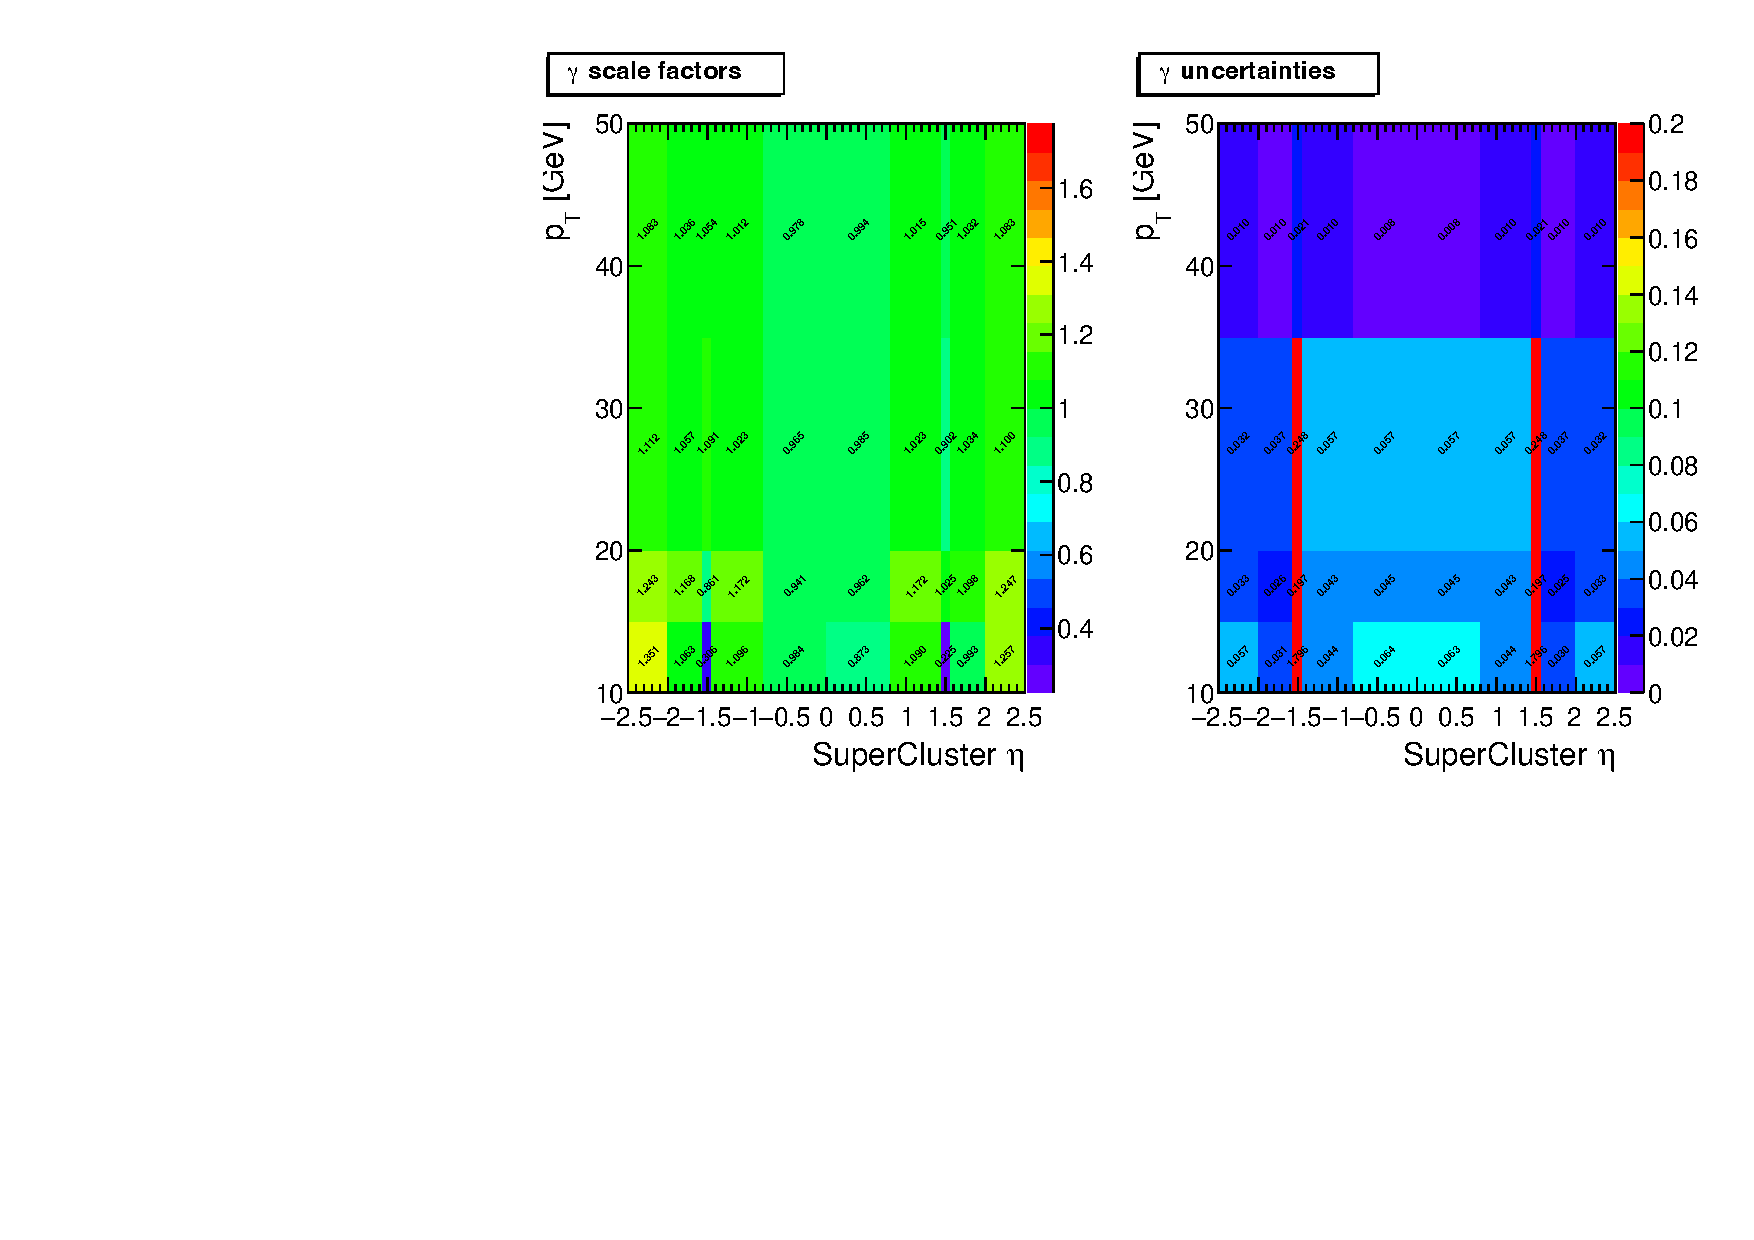
\includegraphics[width=0.8\textwidth]{figures/chapter04/phoID_eff_2016preVFP.pdf}\\
    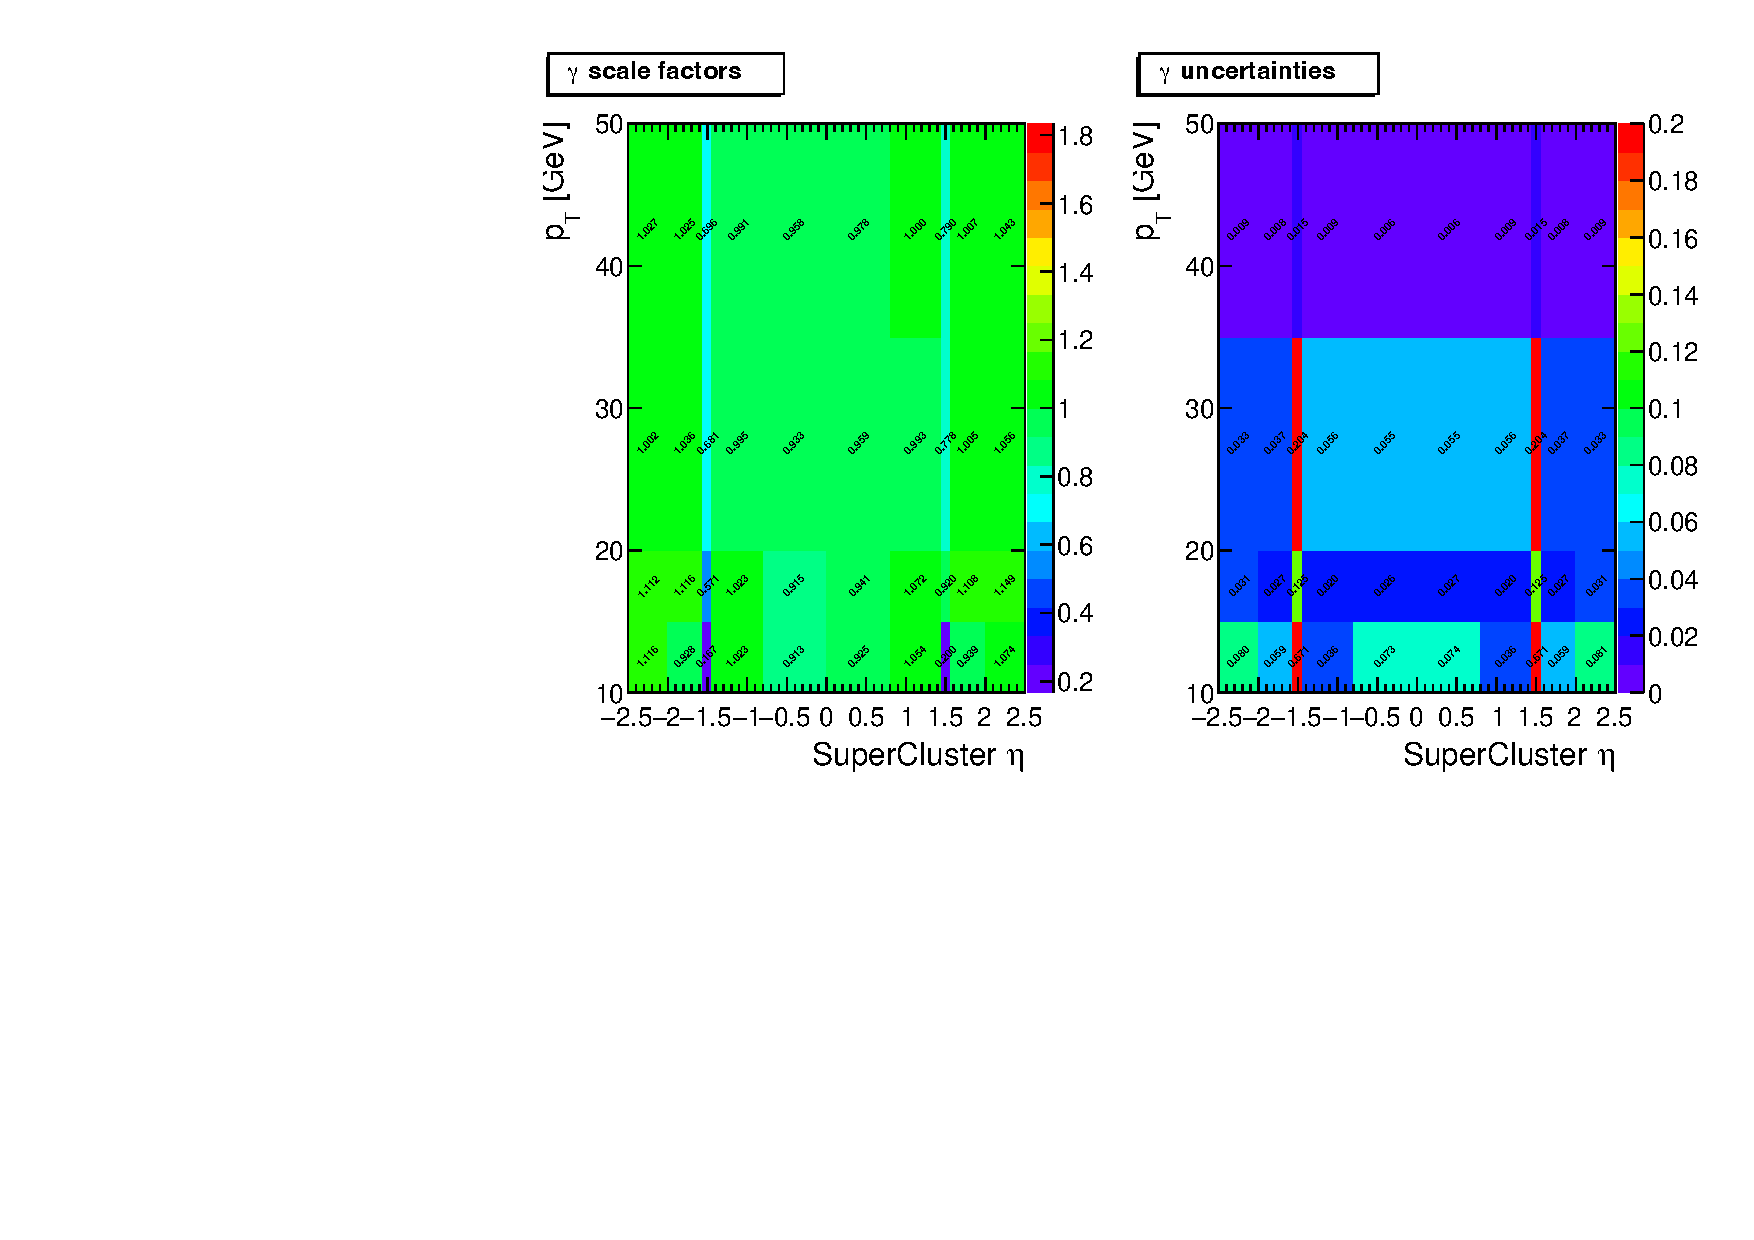
\includegraphics[width=0.8\textwidth]{figures/chapter04/phoID_eff_2016postVFP.pdf} \\
    \bicaption{\quad \centering 左边:所有数据相对于模拟的光子SFs作为$\pt$和$\eta$的函数。右边:数据相对于模拟的光子SFs的不确定性作为$\pt$和$\eta$的函数。顶部显示了2016年pre-VFP的结果,底部显示了2016年post-VFP的结果}{\quad \centering Left: Overall data to simulation scale factors for photons, as function of $\pt$ and $\eta$. Right: Uncertainties on data to simulation scale factors for photons, as a function of $\pt$ and $\eta$. Results are shown for 2016 pre-VFP (top), 2016 post-VFP (bottom)}
    \label{fig:PhoIDEff_1}
\end{center}
\end{figure}

\begin{figure}[htbp]
  \begin{center}
		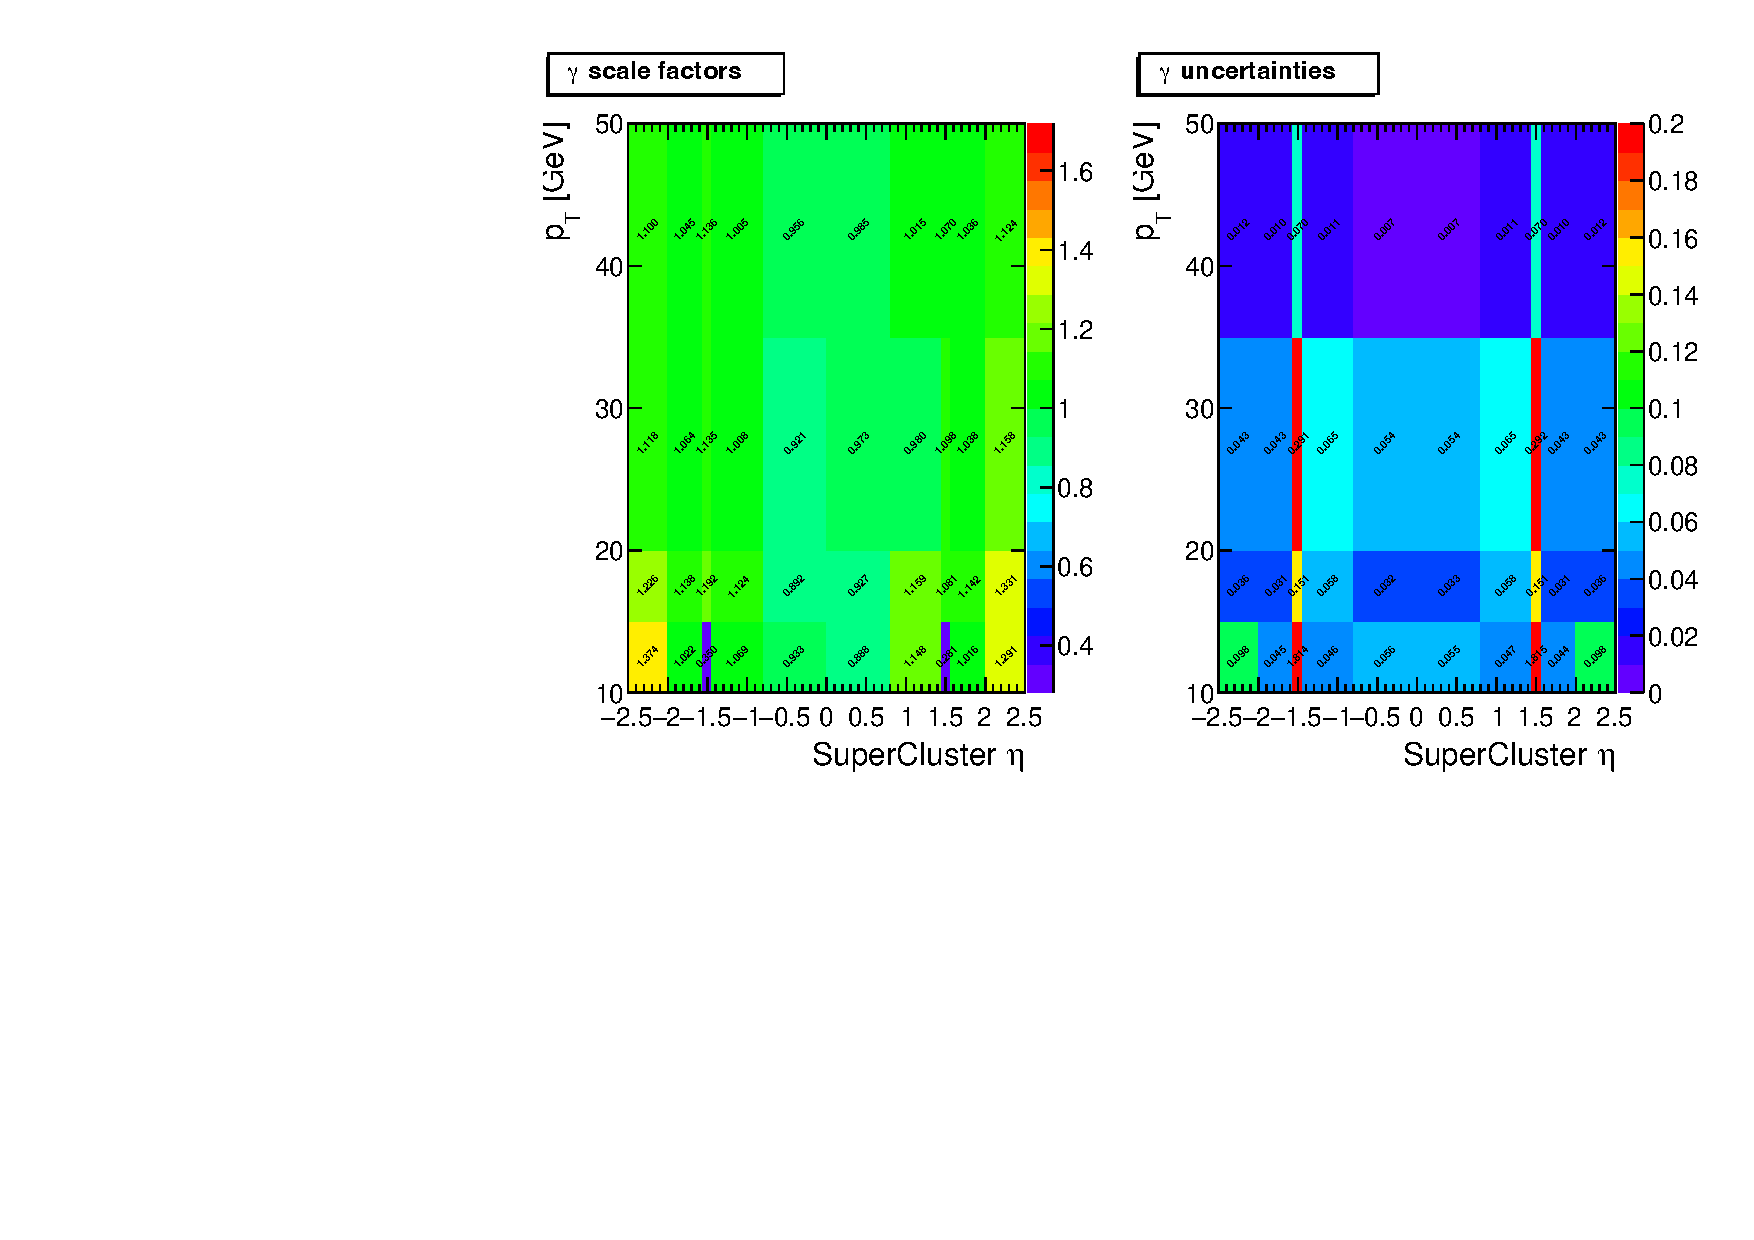
\includegraphics[width=0.8\textwidth]{figures/chapter04/phoID_eff_2017.pdf}\\
		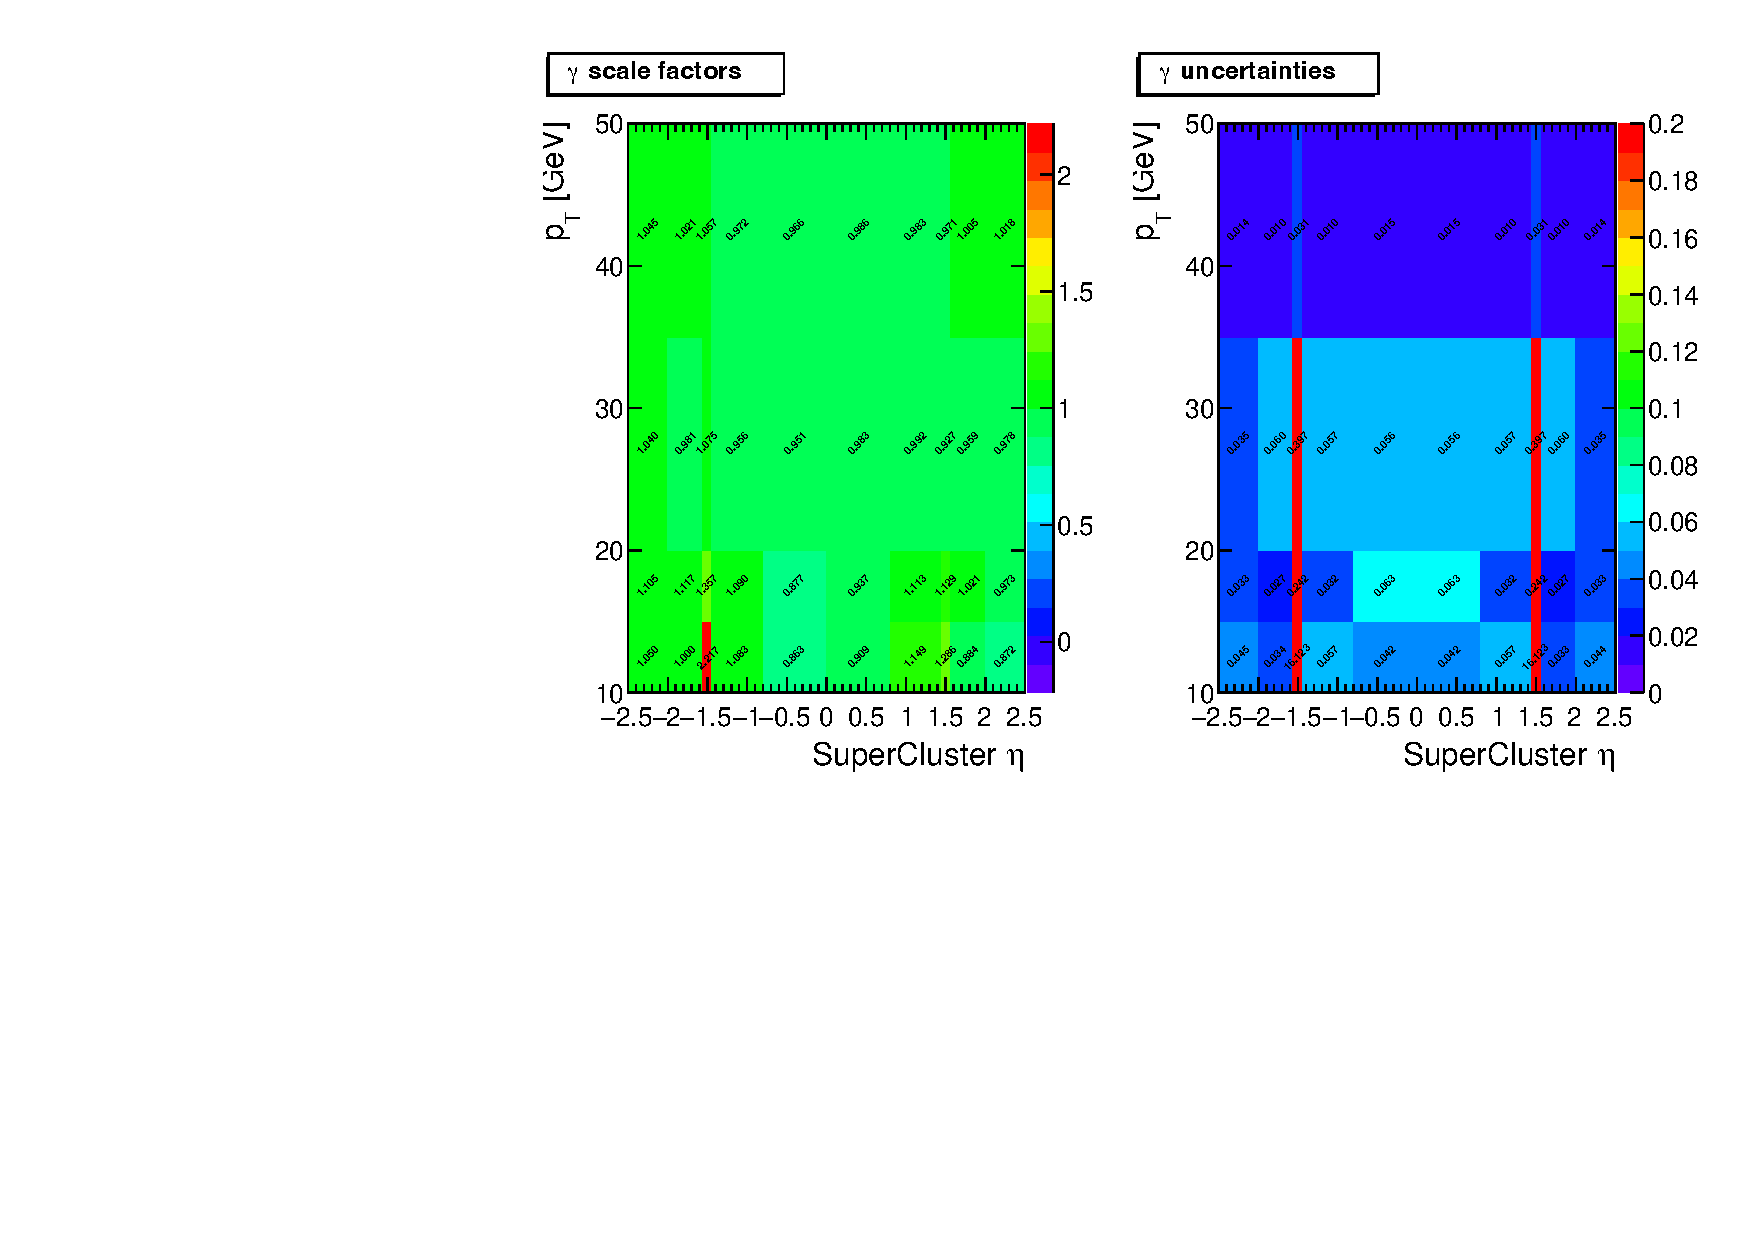
\includegraphics[width=0.8\textwidth]{figures/chapter04/phoID_eff_2018.pdf}\\
    \bicaption{\quad \centering 左边:所有数据相对于模拟的光子SFs作为$\pt$和$\eta$的函数。右边:数据相对于模拟的光子SFs的不确定性作为$\pt$和$\eta$的函数。顶部显示了2017年的结果,底部显示了2018年的结果}{\quad \centering Left: Overall data to simulation scale factors for photons, as a function of $\pt$ and $\eta$. Right: Uncertainties on data to simulation scale factors for photons, as a function of $\pt$ and $\eta$. Results are shown for 2017 (top) and 2018 (bottom)}
    \label{fig:PhoIDEff_2}
\end{center}
\end{figure}

图~\ref{fig:PhoIDEff_1}和图~\ref{fig:PhoIDEff_2}展示了整个Run2三年的SFs和对应的误差。其中,误差的计算考虑了以下来源:
\begin{itemize}
    \item 来自数据样本统计涨落的误差;
    \item 来自蒙卡样本统计涨落的误差;
    \item 来自本底模型的误差:拟合所使用的本底模型的形状会对最终的效率计算产生影响,进而影响最终的SFs。这部分误差可以通过使用不同形状的本底模型进行拟合来估算,在这个过程中信号模型保持不变,本底模型由原来的误差函数和指数函数的卷积改变为指数函数或者Power-Low函数。
    \item 来自信号模型的误差:拟合所使用的信号模型的形状同样也会对最终的SFs计算产生影响。与估计本底模型的误差相似,可以通过改变信号模型的形状来对这一部分误差进行估计。在这个过程中,本底模型的形状保持不变,信号模型由原来的蒙卡形状和高斯函数的卷积改变为Double Crystall Ball函数和高斯函数的卷积。
    \item 来自tag电子筛选引起的误差:这部分误差可以通过改变tag电子的筛选条件重新计算效率和SFs来进行估计。在估计的过程中,将tag电子的定义改变为通过medium工作点并且$\pt>25\GeV$。
    \item 来自蒙卡样本产生子引起的误差:使用不同的产生子产生出来的蒙卡样本会具有细微的差别。由于在拟合中信号模型利用了蒙卡样本的形状,因此使用不同产生子的蒙卡样本会影响最终的SFs的计算。这部分误差可以通过使用由不同产生子所产生的蒙卡样本来进行估算。
\end{itemize}

总的误差是以上所有误差来源项的平方和开根号。在本分析中,大部分光子的横动量都集中在30$\GeV$以下,对应的SFs的计算误差平均在5\%左右,其中占主导的误差来源是蒙卡样本产生子引起的误差。原因是由于Z玻色子衰变产生的电子横动量比较高,在低动量区域内的样本事例数比较少,统计涨落较大,因此更换不同产生子的蒙卡样本后会产生较大的影响。但是由于本分析是对Higgs稀有衰变过程的寻找,在最终的分析结果中数据的统计误差占主导,光子效率的误差仅产生次要的影响,详细分析结果见第~\ref{sec:Sys}节。

\section{事例筛选}\label{sec:EventSelect}

表格~\ref{tab:objsummary}总结了本分析中使用的所有物理对象的筛选条件,包括:电子、缪子、FSR光子以及光子。在对所有物理对象重建完成之后,可以利用这些物理对象重建出我们所感兴趣的事例。在本分析中,Higgs通过一个Z玻色子和一个类轴子作为中间态衰变到两个轻子加两个光子,因此可以通过两个轻子重建出Z玻色子、通过两个光子重建出类轴子,进而再利用Z玻色子和类轴子重建出Higgs粒子。具体重建步骤如下:
\begin{enumerate}
    \item Trigger 筛选:首先要求事例通过第~\ref{sec:Trigger}节描述的触发条件,要求筛选的事例含有至少一个轻子或者两个轻子。
    \item Z玻色子候选体筛选:要求事例含有至少一对味道相同带电相反的轻子($e^{+}e^{-}, \mu^{+}\mu^{-}$),这些轻子包含了相应的FSR光子并且通过了所有轻子的筛选条件。然后利用这些轻子对重建出Z玻色子候选体。其中,要求两个筛选出来的电子(缪子)满足$\mathrm{p_{T, Leading}>25 (20)\GeV}$,$\mathrm{p_{T, Sub-leading}>15 (10)\GeV}$,这些阈值的选择主要由触发决定。
    \item ALPs候选体筛选:要求事例中含有两个通过光子ID的光子,利用这两个光子重建出类轴子候选体。其中,要求这两个光子的横动量$\pt>10\GeV$,这主要是由CMS探测器中对光子重建所需的最低横动量所决定。
    \item Higgs候选体筛选:最后,利用Z玻色子候选体和类轴子候选体重建出Higgs候选体,选中的事例要求满足以下条件:
        \begin{itemize}
            \item Z玻色子的质量$m_{Z}>50\GeV$,用以排除$\gamma^{*}\rightarrow\ell\ell$这部分本底。
            \item 轻子和光子之间的距离$\dR(l,\gamma)>0.4$。
            \item 由于本分析要求一个在壳的Z玻色子和两个横动量大于10$\GeV$的光子,使得本底的$\mllgg$分布会在110$\GeV$附近出现了turn-on(不变质量谱的分布在110$\GeV$以下呈上升趋势,然后在110$\GeV$附近达到极大值,而后又呈下降趋势),为了使得本底建模的时候可以正确描述这部分turn-on并且拟合区间具有足够的边带区域,要求选出的Higgs候选体质量$95<\mllgg<180\GeV$。
        \end{itemize}
\end{enumerate}

\begin{table}[H]
	\centering
	\bicaption{\quad \centering 物理对象选择汇总}{\quad \centering Summary of physics object selection}
	\resizebox{\textwidth}{!}{
	\begin{tabular}{cc}
		\hline
		\multicolumn{2}{c}{\textbf{Electrons}} \\ \hline
		\multicolumn{2}{c}{$\mathrm{p_T^e} > 7 $~\si{\GeV} \hspace{0.5cm} $|\eta^e| < 2.5$}   \\
		\multicolumn{2}{c}{$\mathrm{d_{xy}} < 0.5 \, \mathrm{cm}$ \hspace{0.5cm} $\mathrm{d_{z}} < 1 \, \mathrm{cm}$}                  \\
		\multicolumn{2}{c}{$| {\rm SIP_{3D}} | < 4$ }  \\
        \multicolumn{2}{c}{BDTs ID with isolation with cuts }  \\ \hline \hline
		\multicolumn{2}{c}{\textbf{Muons}}  \\ \hline
        \multicolumn{2}{c}{Global or Tracker Muon} \\
		\multicolumn{2}{c}{$\mathrm{p_{T}^{\mu}} > 5$~\si{\GeV} \hspace{0.5cm} $|\eta^{\mu}| < 2.4$}   \\
		\multicolumn{2}{c}{$\mathrm{d_{xy}} < 0.5 \, \mathrm{cm}$ \hspace{0.5cm} $\mathrm{d_{z}} < 1 \, \mathrm{cm}$}           \\
		\multicolumn{2}{c}{$| {\rm SIP_{3D}} | < 4$  }  \\
		\multicolumn{2}{c}{PF muon ID if $\pt<200$~\si{\GeV}, PF muon ID or High-$\pt$ muon ID if $\pt>200$~\si{\GeV}}      \\
        \multicolumn{2}{c}{$\ensuremath{{\cal I}_{\mathrm{PF}}^{\mu}} < 0.35$}    \\ \hline \hline
		\multicolumn{2}{c}{\textbf{FSR photons}}    \\ \hline
		\multicolumn{2}{c}{$\mathrm{p_T^{\gamma}} > 2 \GeV$ \hspace{0.5cm} $|\eta^{\gamma}| < 2.4$}     \\
		\multicolumn{2}{c}{$\ensuremath{{\cal I}_{\mathrm{PF}}^{\gamma}} < 1.8$}        \\
		\multicolumn{2}{c}{$\Delta R(\ell,\gamma) < 0.5$ \hspace{0.5cm} $\frac{\Delta R(\ell,\gamma)}{(\pt^{\gamma})^2} < 0.012 \GeV^{-2}$}     \\ \hline \hline
		\multicolumn{2}{c}{\textbf{Photons}}    \\ \hline
		\multicolumn{2}{c}{$10 < \mathrm{p_T^{\gamma}} < 14 \GeV$ \hspace{0.2cm} $H/E < 0.15\ \&\&\ I_{ch} < 10\GeV$}     \\
		\multicolumn{2}{c}{or}     \\
		\multicolumn{2}{c}{$\mathrm{p_T^{\gamma}} > 14 \GeV$ \hspace{0.5cm} $H/E < 0.15$}     \\
		\multicolumn{2}{c}{Modified tight photon cut-based ID}     \\ \hline
	\end{tabular}}
	\label{tab:objsummary}
\end{table}

\begin{figure}[htbp]
  \begin{center}
		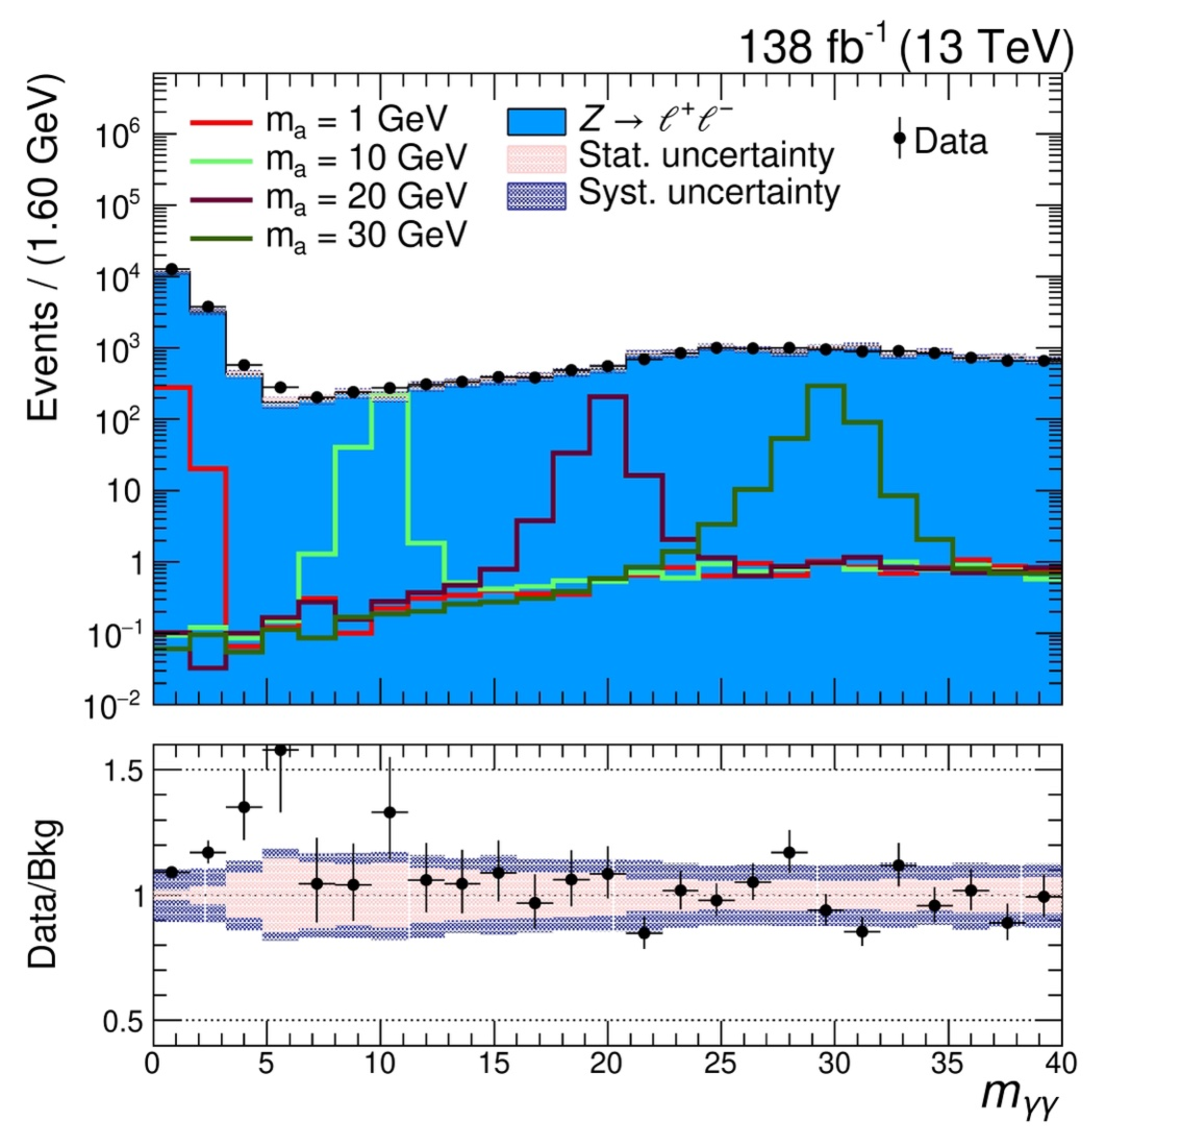
\includegraphics[width=0.5\textwidth]{figures/chapter04/BDT_input/ALP_m_log.pdf}
    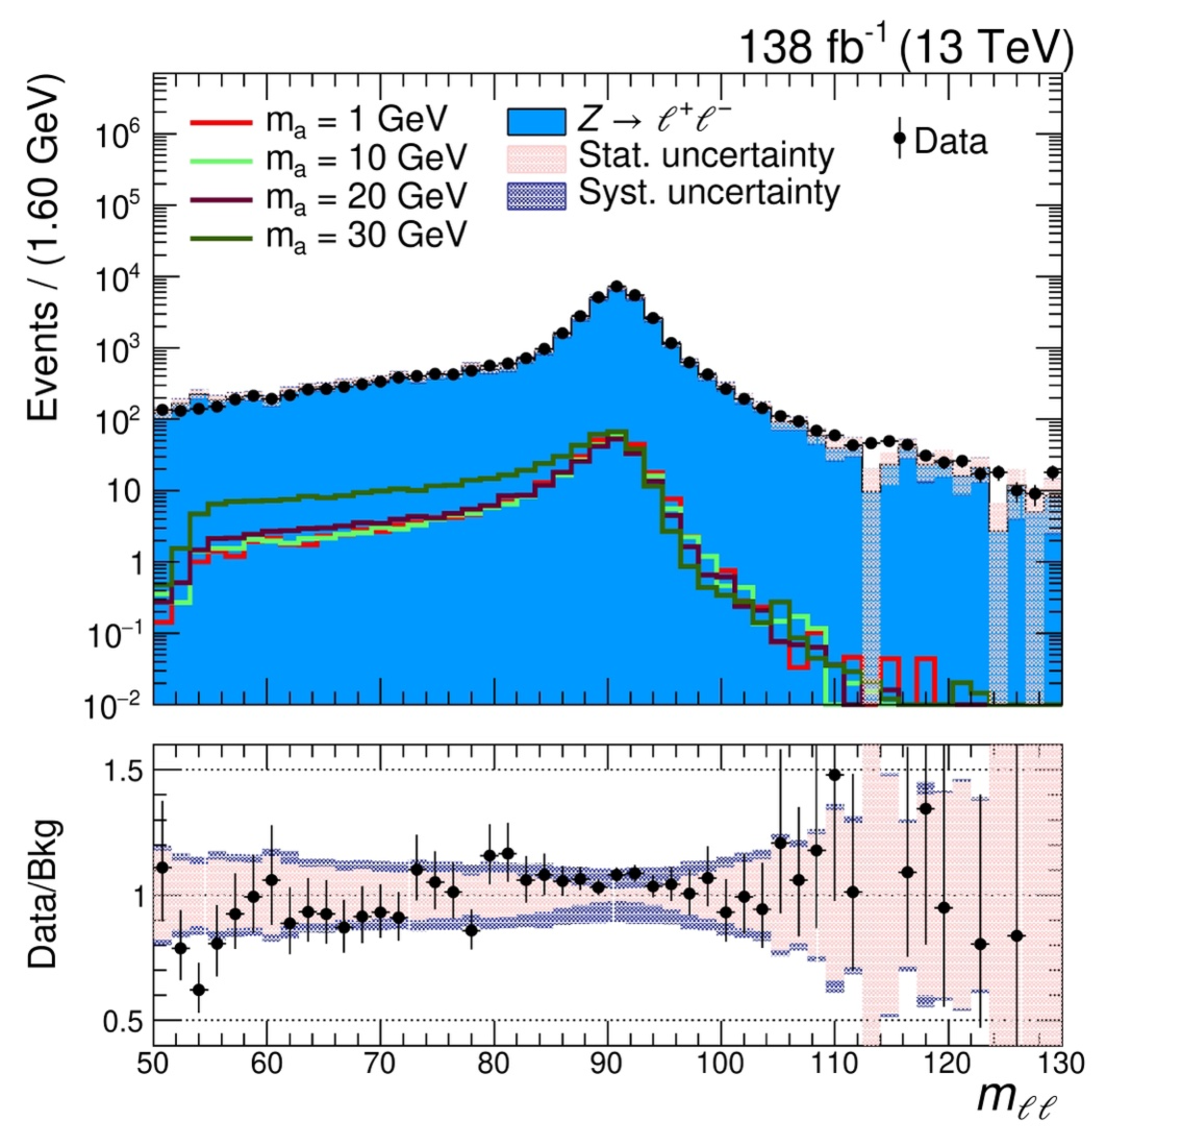
\includegraphics[width=0.5\textwidth]{figures/chapter04/BDT_input/Z_m_log.pdf} 
		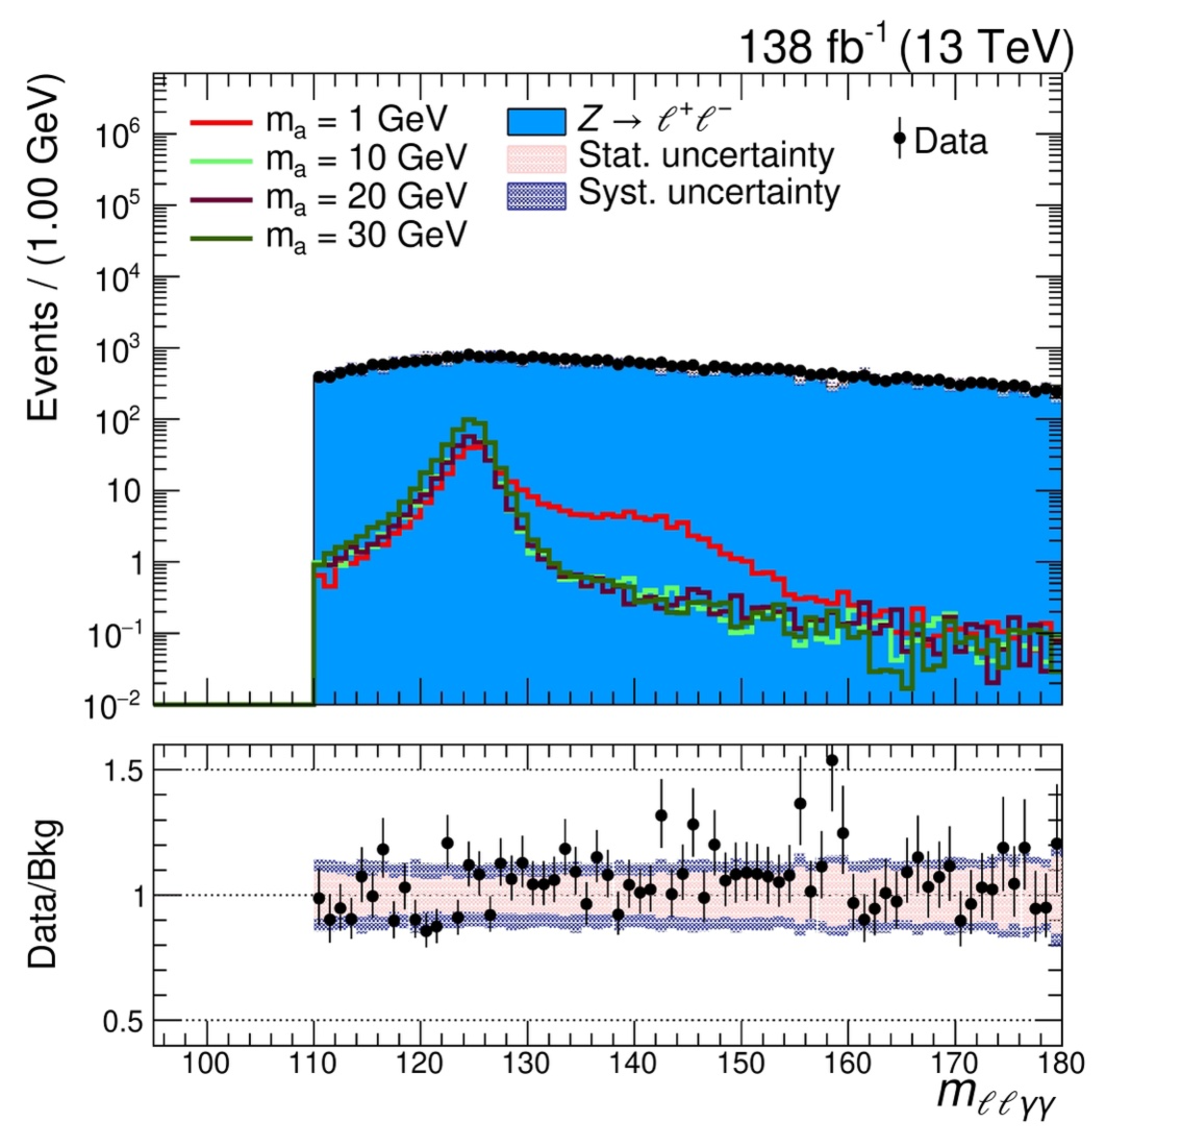
\includegraphics[width=0.5\textwidth]{figures/chapter04/BDT_input/H_m_log.pdf}
    \bicaption{\quad \centering 通过事例筛选后的ALPs候选体(上图)、Z候选体(中图)和Higgs候选体(下图)的不变质量分布}{\quad \centering Invariant mass distribution after all of the event selections applied for ALPs candidate (top), Z candidate (middle), and Higgs candidate (bottom)}
    \label{fig:mass}
\end{center}
\end{figure}

图~\ref{fig:mass}展示了通过事例筛选后重建出的ALPs候选体、Z候选体和Higgs候选体的不变质量分布图,信号用不同颜色的空心直方图表示,黑色的点代表数据,蓝色的填充直方图表示本底蒙卡样本的分布,图中的系统误差包括了光子效率误差、轻子效率误差以及堆积事例的影响。图~\ref{fig:SelectionEff}展示了不同年份的信号样本通过事例筛选的效率分布图,最终信号的筛选效率大约为2.5\%。

\begin{figure}[htbp]
  \begin{center}
		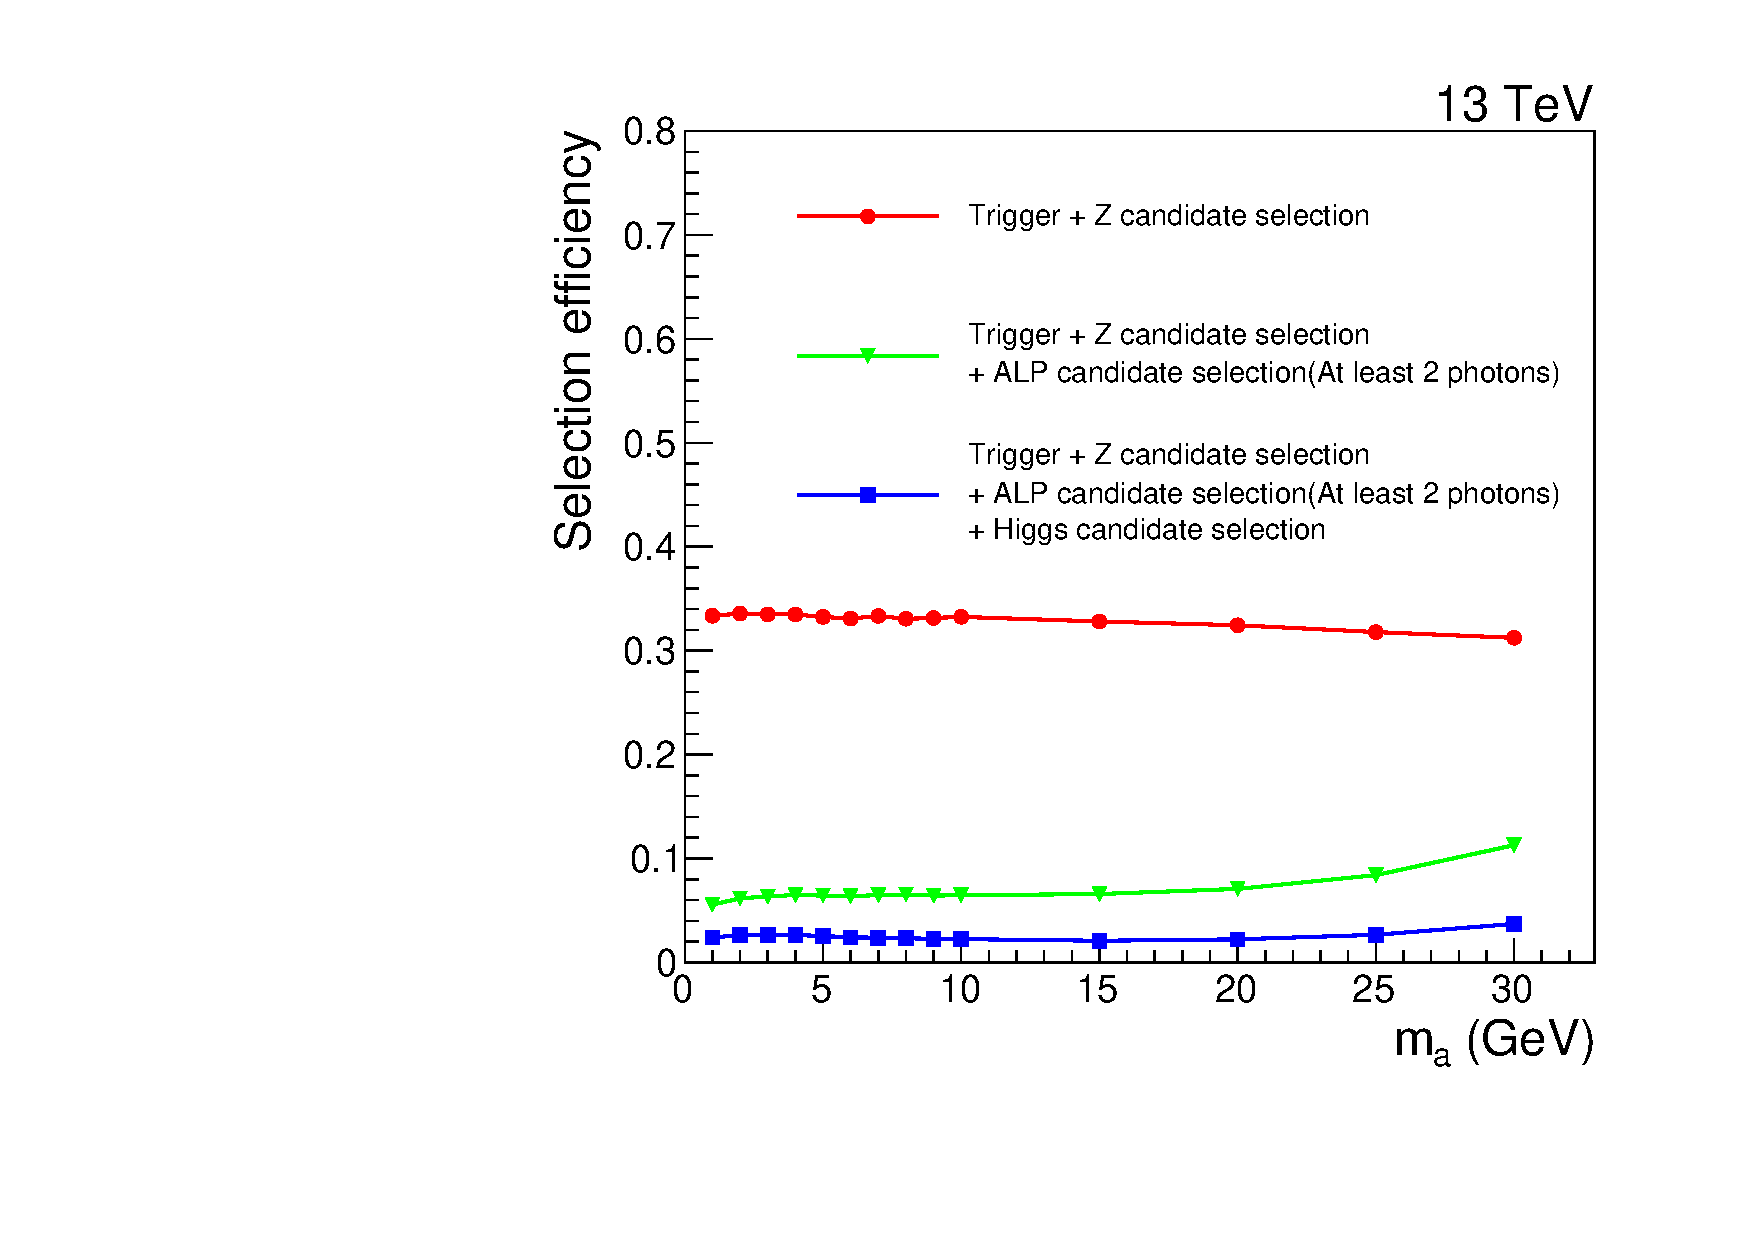
\includegraphics[width=0.42\textwidth]{figures/chapter04/cuteff_16.pdf}
    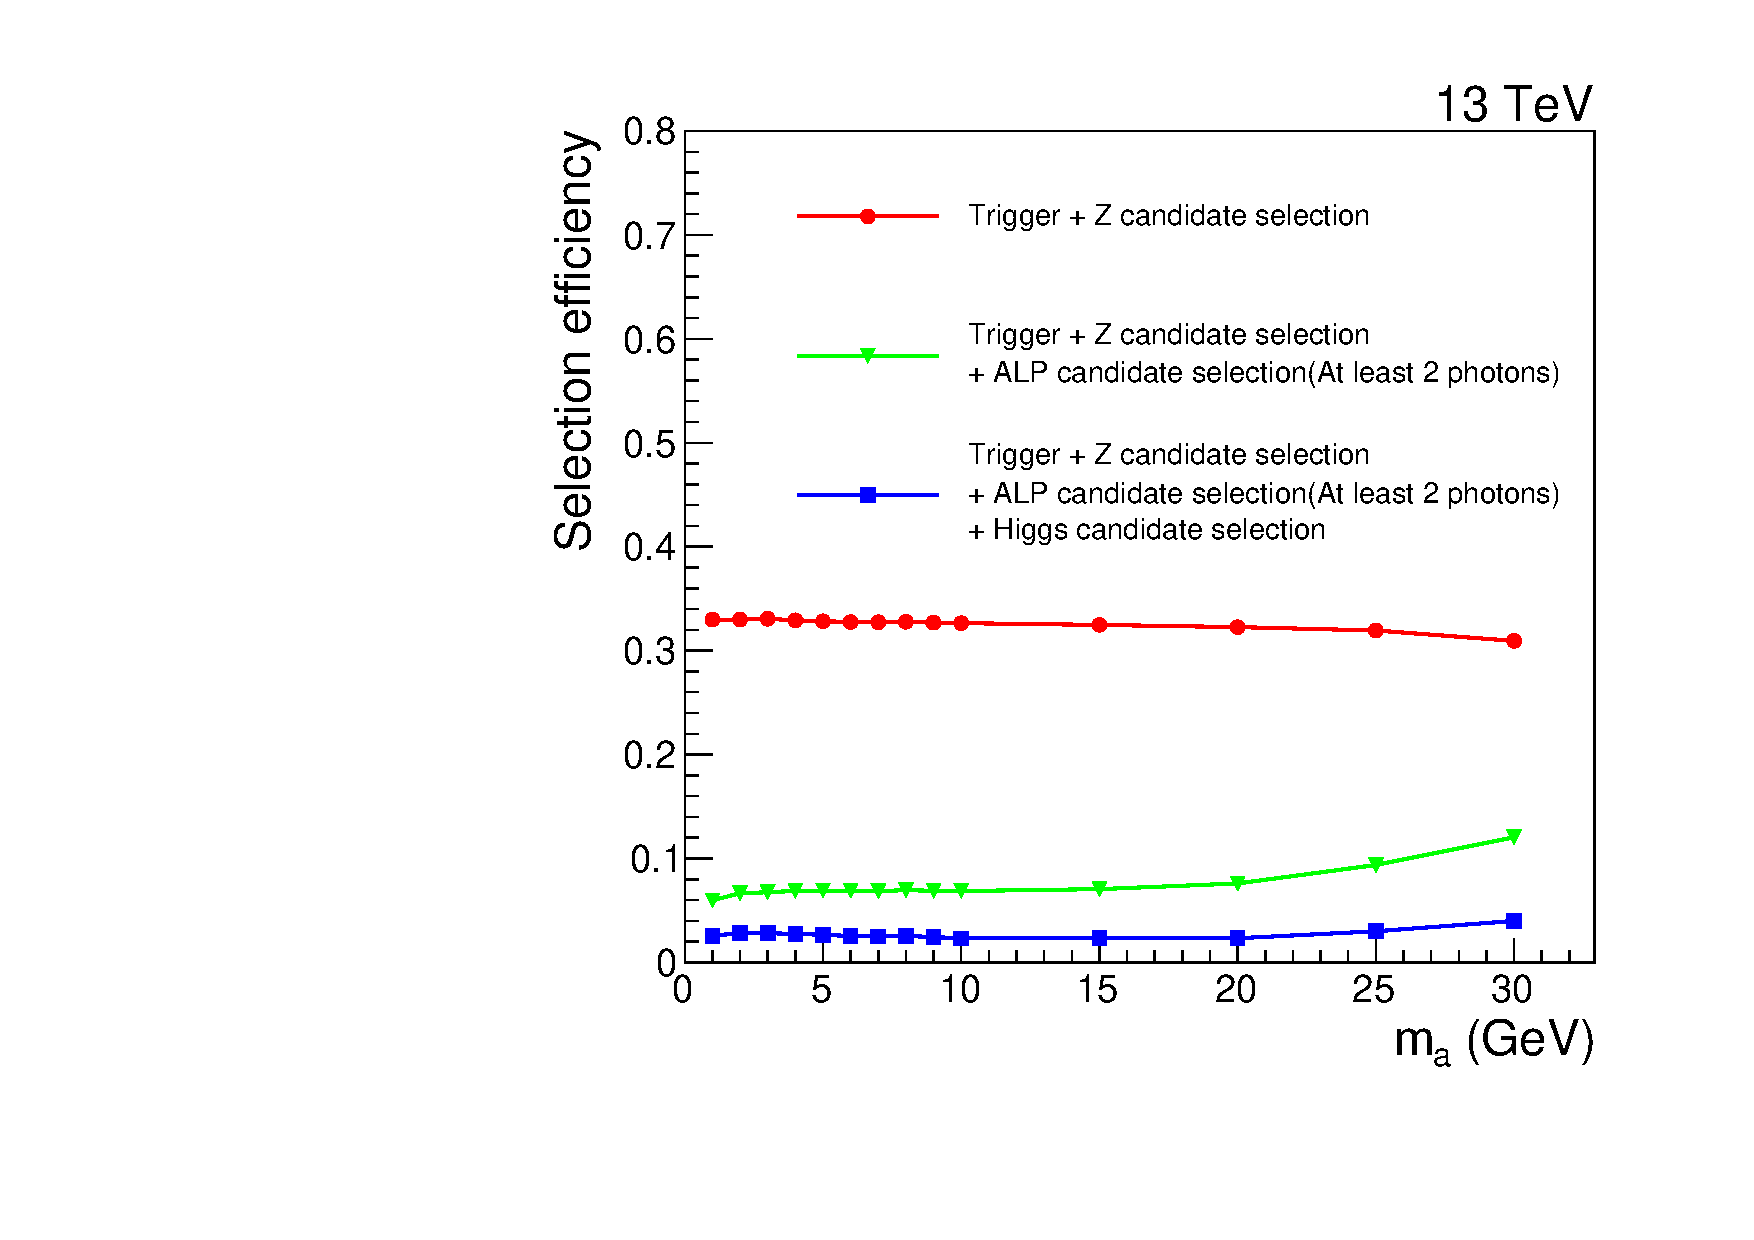
\includegraphics[width=0.42\textwidth]{figures/chapter04/cuteff_16APV.pdf} \\
		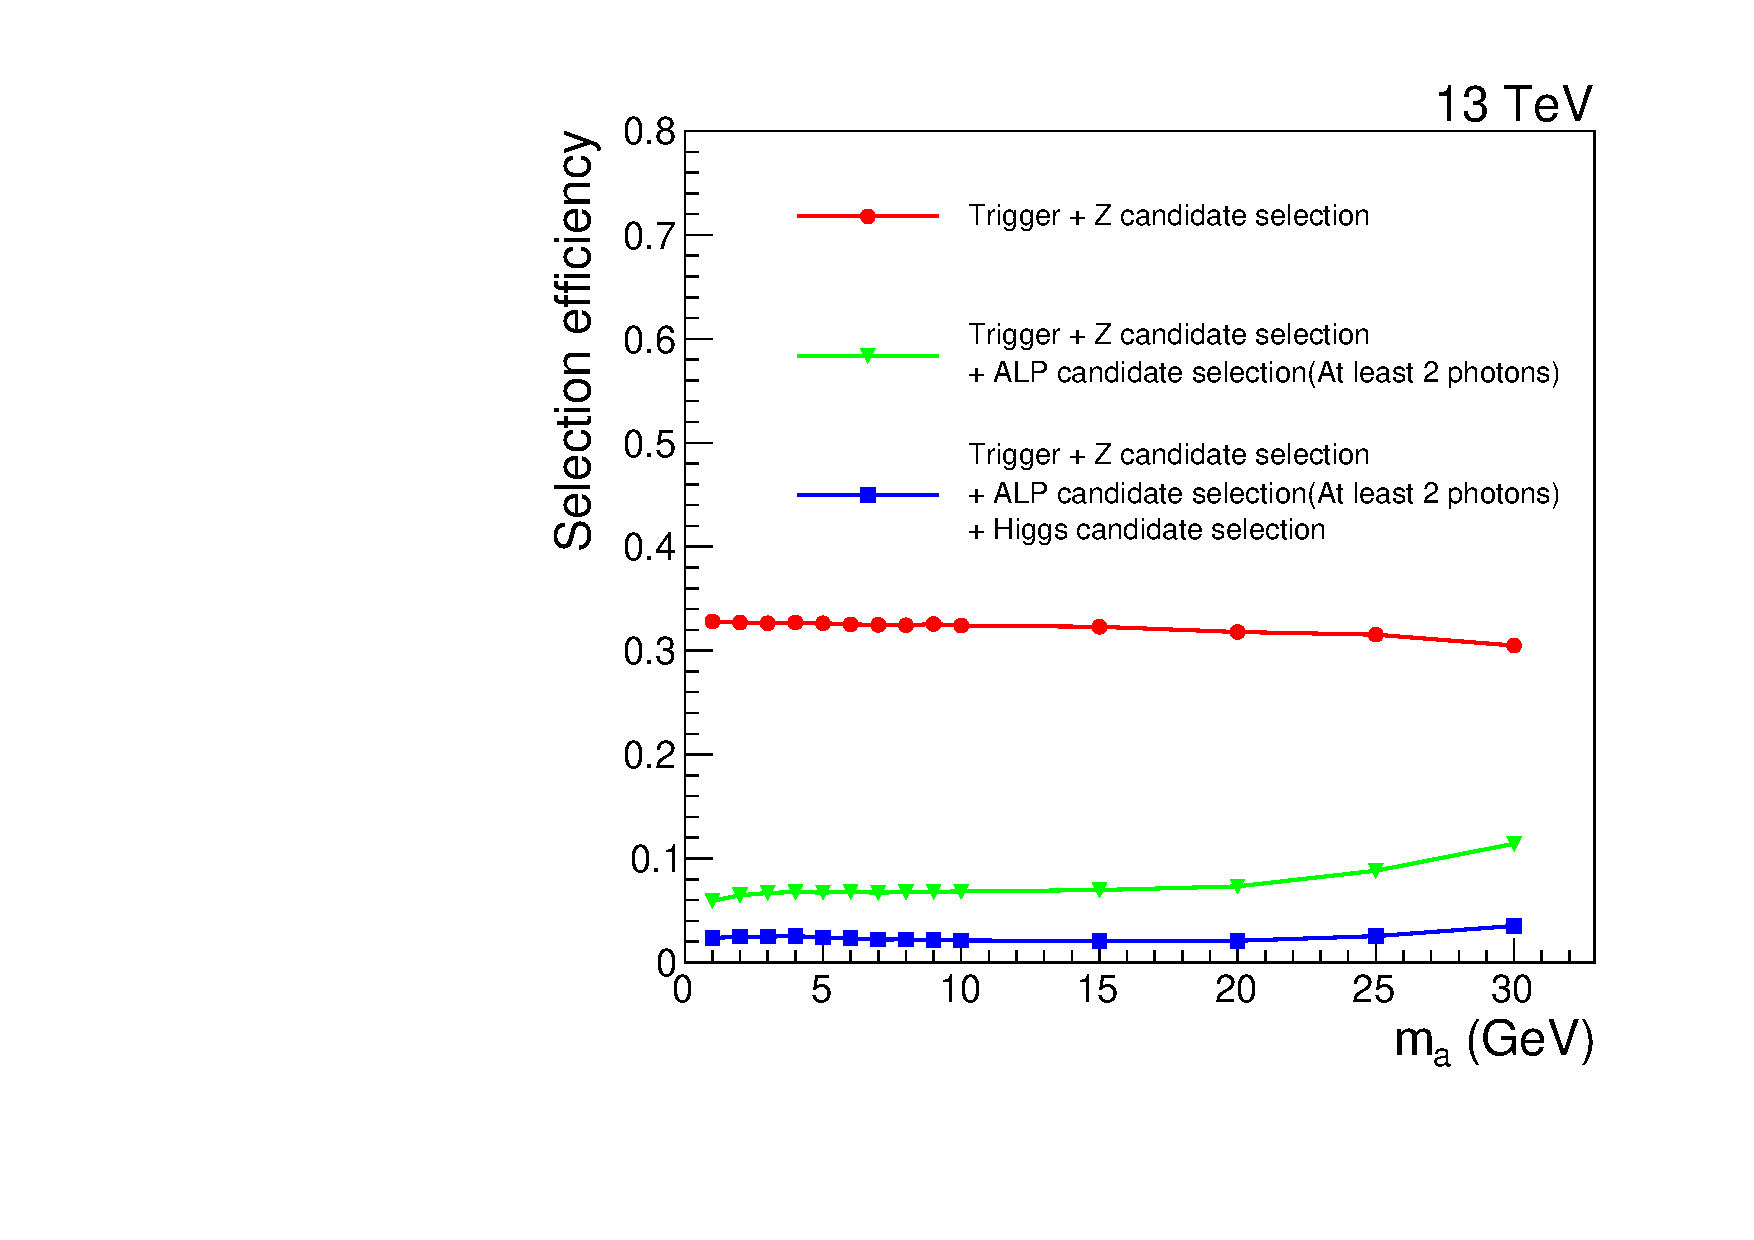
\includegraphics[width=0.42\textwidth]{figures/chapter04/cuteff_17.pdf}
		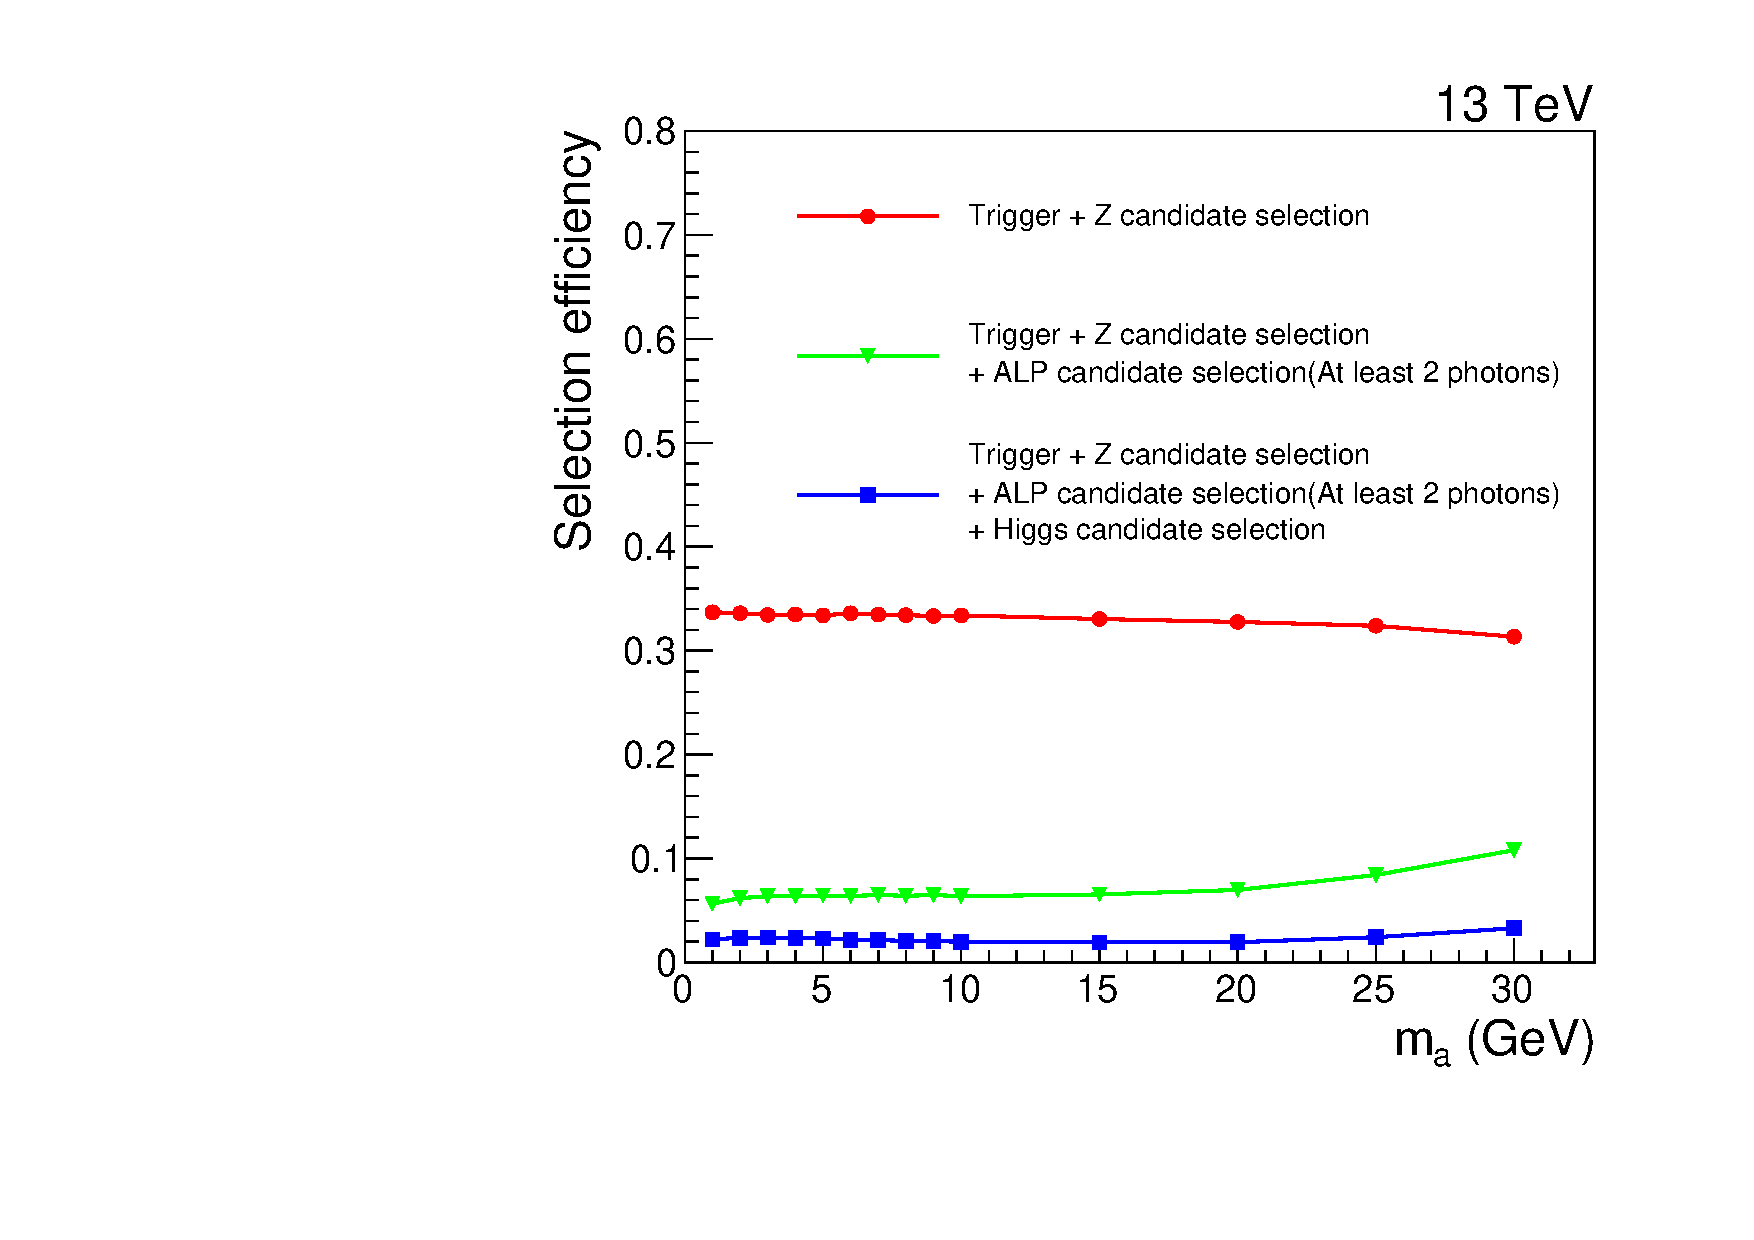
\includegraphics[width=0.42\textwidth]{figures/chapter04/cuteff_18.pdf}\\
    \bicaption{\quad \centering 信号事例的筛选效率,左上为2016年 post-VFP、右上为2016年 pre-VFP、左下为2017年、右下为2018年的结果}{\quad \centering The results of signal selection efficiency for 2016 post-VFP (top left), 2016 pre-VFP (top right), 2017 (bottom left), and 2018 (bottom right)}
    \label{fig:SelectionEff}
\end{center}
\end{figure}



\section{决策树法优化事例筛选}\label{sec:BDT}

为了进一步区分信号和本底,本分析采取了多变量分析(MVA)的策略,使用XGBoost软件包~\cite{XGBoost}中的提升决策树分类器来对信号和本底进行区分。此策略利用了已知类别的信号和本底事例,通过输入事例的变量信息来对提升决策树进行训练,得到能够区分信号和本底的最优模型。而后,将训练好的提升决策树模型应用于数据中,进而可以非常好的降低本底事例的影响,有效的提升信噪比。在本分析中,主要本底过程来自于标准模型Drell-Yan过程,因此,训练所使用的本底样本由Drell-Yan样本构成。

\begin{table}[h]
  \begin{center}
  \bicaption{\quad \centering 对提升决策树样本的处理}{\quad \centering Processes of BDTs samples}
    \scriptsize
    \begin{tabular}{lcc} \hline
        & Signal & Background \\ \hline
       Training & All mass points together (30\%) & $Z\rightarrow\ell\ell$ (60\%) \\ \hline
       Testing & All mass points together (20\%) & $Z\rightarrow\ell\ell$ (40\%) \\ \hline
       Application & All mass points together (50\%) & Data Driven \\
       (Signal modeling and limit evaluation) &  & \\ \hline
    \end{tabular}
    \label{tab:process}
  \end{center}
\end{table}

为了避免在对提升决策树进行训练、评估和应用的过程中产生关联,本分析将所有样本随机的分成了若干子样本,分别用于提升决策树的训练(Training)、评估(Testing)和应用(Application)。表格~\ref{tab:process}展示了用于训练、评估和应用的样本占总样本的比例。对于信号样本,所有质量点的样本都合并到了一起用于训练,应用样本仅仅用于信号模型的构建以及最终信号的提取。对于本底样本,由于最终的信号提取采取了数据驱动的方法,因此MC样本仅用于提升决策树的训练和评估。同时,为了增加训练过程中的样本统计量,本分析将三年的样本合并到一起用于训练。

\subsection{输入变量}

由于最终的信号提取是通过对$m_{\ell\ell\gamma\gamma}$的分布进行拟合所得到的,为了信号提取的方便,我们希望最终的本底分布是一个光滑平坦的分布。因此,本分析要求训练所使用的所有输入变量和$m_{\ell\ell\gamma\gamma}$之间不存在较强的关联性。本分析用于提升决策树训练所使用的输入变量定义如下:
\begin{itemize}
    \item 两个光子的横动量:$p_{T,\gamma1}$和$p_{T,\gamma2}$(其中,$\gamma1$和$\gamma2$分别表示横动量最大和次大的光子);
    \item 两个光子的$R_9$:$R_{9,\gamma1}$和$R_{9,\gamma2}$;
    \item 两个光子的$\sigma_{i\eta i\eta}$:$\sigma_{i\eta i\eta,\gamma1}$和$\sigma_{i\eta i\eta,\gamma2}$;
    \item 两个光子的PF光子隔离度:$I_{\gamma,\gamma1}$和$I_{\gamma,\gamma2}$;
    \item ALPs的PF光子隔离度$I_{\gamma,ALPs}$:对重建出的ALPs候选体周围半径$\dR<0.3$的锥形体内的所有PF光子横动量求和;
    \item 重建出的Z玻色子候选体和ALPs候选体之间的角距离:$\Delta R(Z,a)$;
    \item 两个光子之间的角距离:$\Delta R(\gamma1,\gamma2)$;
    \item 横动量最大的光子和Z玻色子候选体之间的角距离:$\Delta R (\gamma1,Z)$;
    \item 重建出的ALPs候选体横动量$\pt$和$m_{\ell\ell\gamma\gamma}$之间的比值:$p_{T,a}/m_{\ell\ell\gamma\gamma}$;
    \item 重建出的Higgs候选体横动量$p_{T,H}$;
\end{itemize}
对于这些变量的选择主要考虑了信号事例和本底事例中光子的动力学分布之间的差异、重建出的类轴子候选体和Z玻色子候选体、Higgs候选体之间的动力学分布之间的差异。由于在第~\ref{sec:EventReco}节中,轻子的选择已经要求了所有的轻子通过tight ID,因此和轻子相关的变量不再引入提升决策树的训练中。图~\ref{fig:BDT_Vars1}、~\ref{fig:BDT_Vars2}、~\ref{fig:BDT_Vars3}展示了这些输入变量的数据和蒙卡的分布情况,蒙卡样本被归一化到了数据所对应的积分亮度,图中所显示的系统误差主要包括了:光子效率误差、轻子效率误差以及堆积事例的影响。从这些分布中可以看到,数据和蒙卡之间的吻合程度非常好。此外,由于本底模型是通过数据驱动的方法直接从数据中拟合得到,数据和蒙卡之间个别微小的偏差并不会影响最终的结果。

\begin{figure}[htbp]
  \begin{center}
		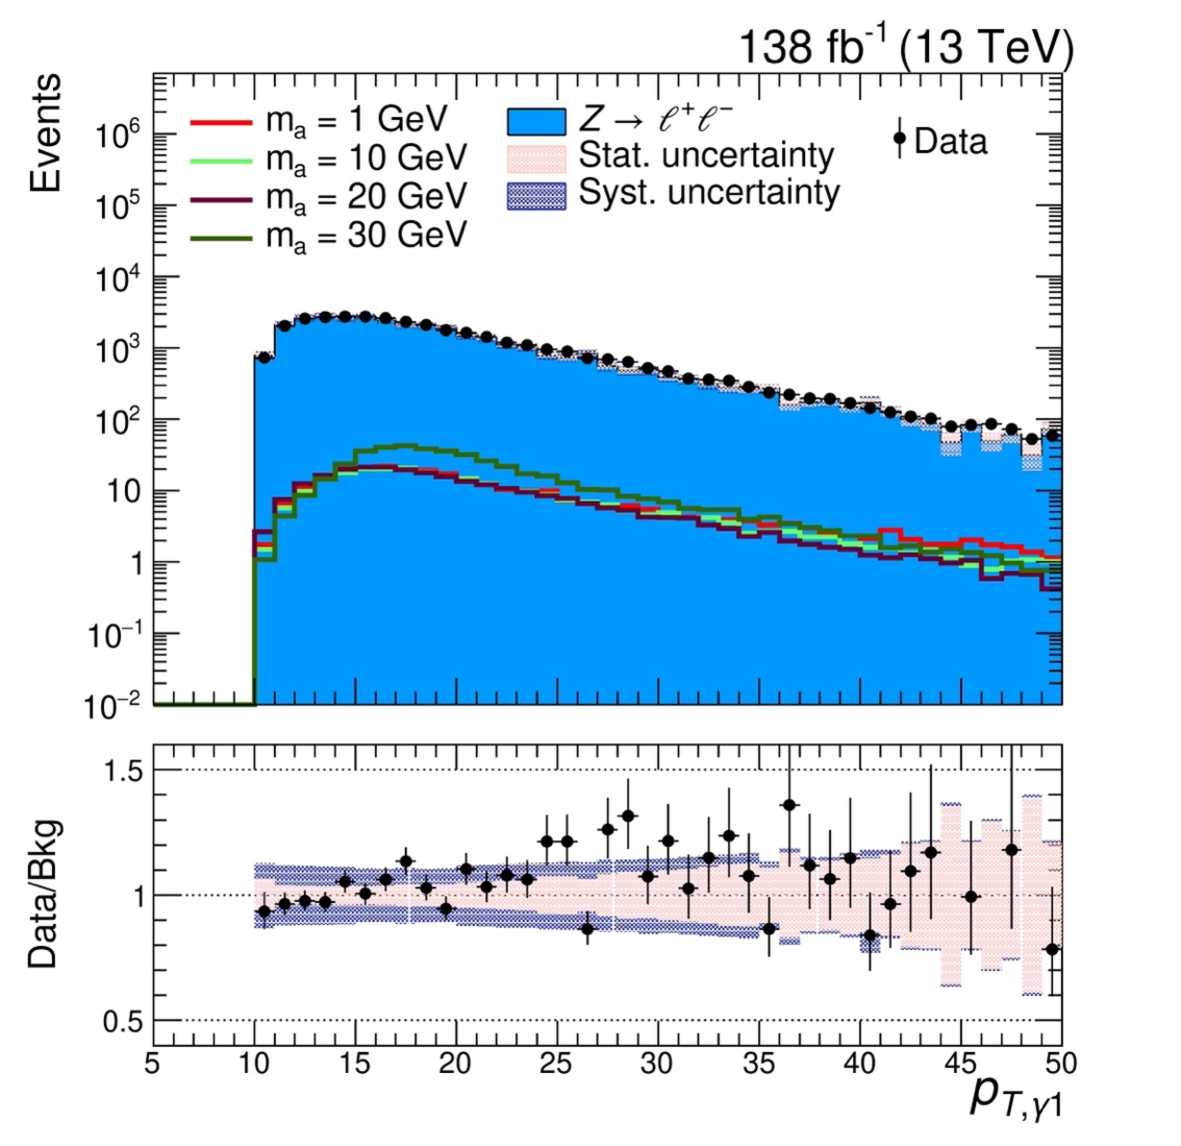
\includegraphics[width=0.42\textwidth]{figures/chapter04/BDT_input/pho1Pt_log.pdf}
    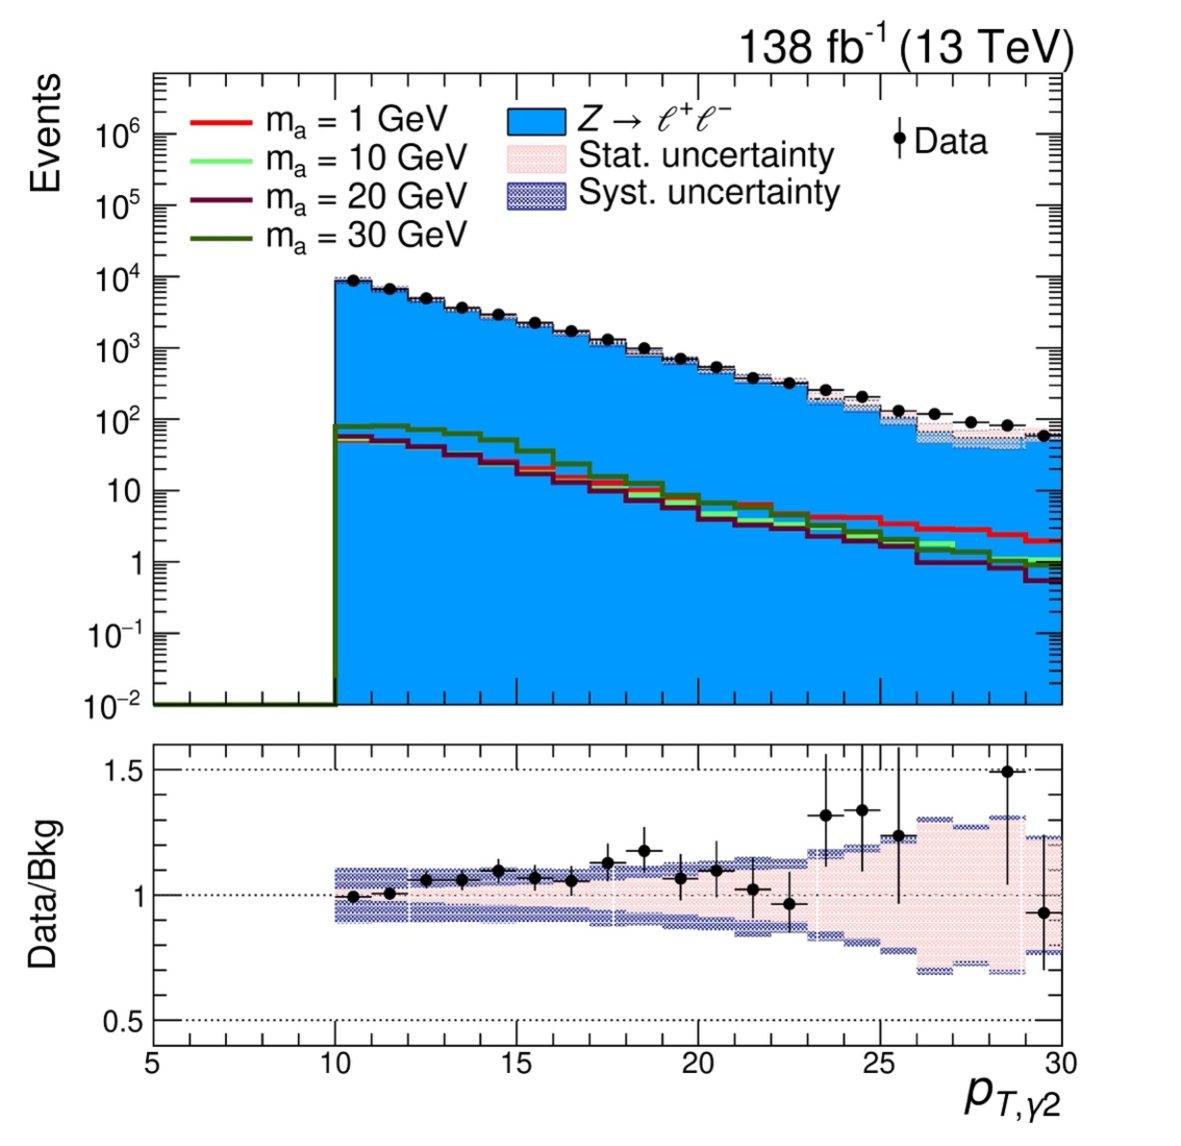
\includegraphics[width=0.42\textwidth]{figures/chapter04/BDT_input/pho2Pt_log.pdf} \\
		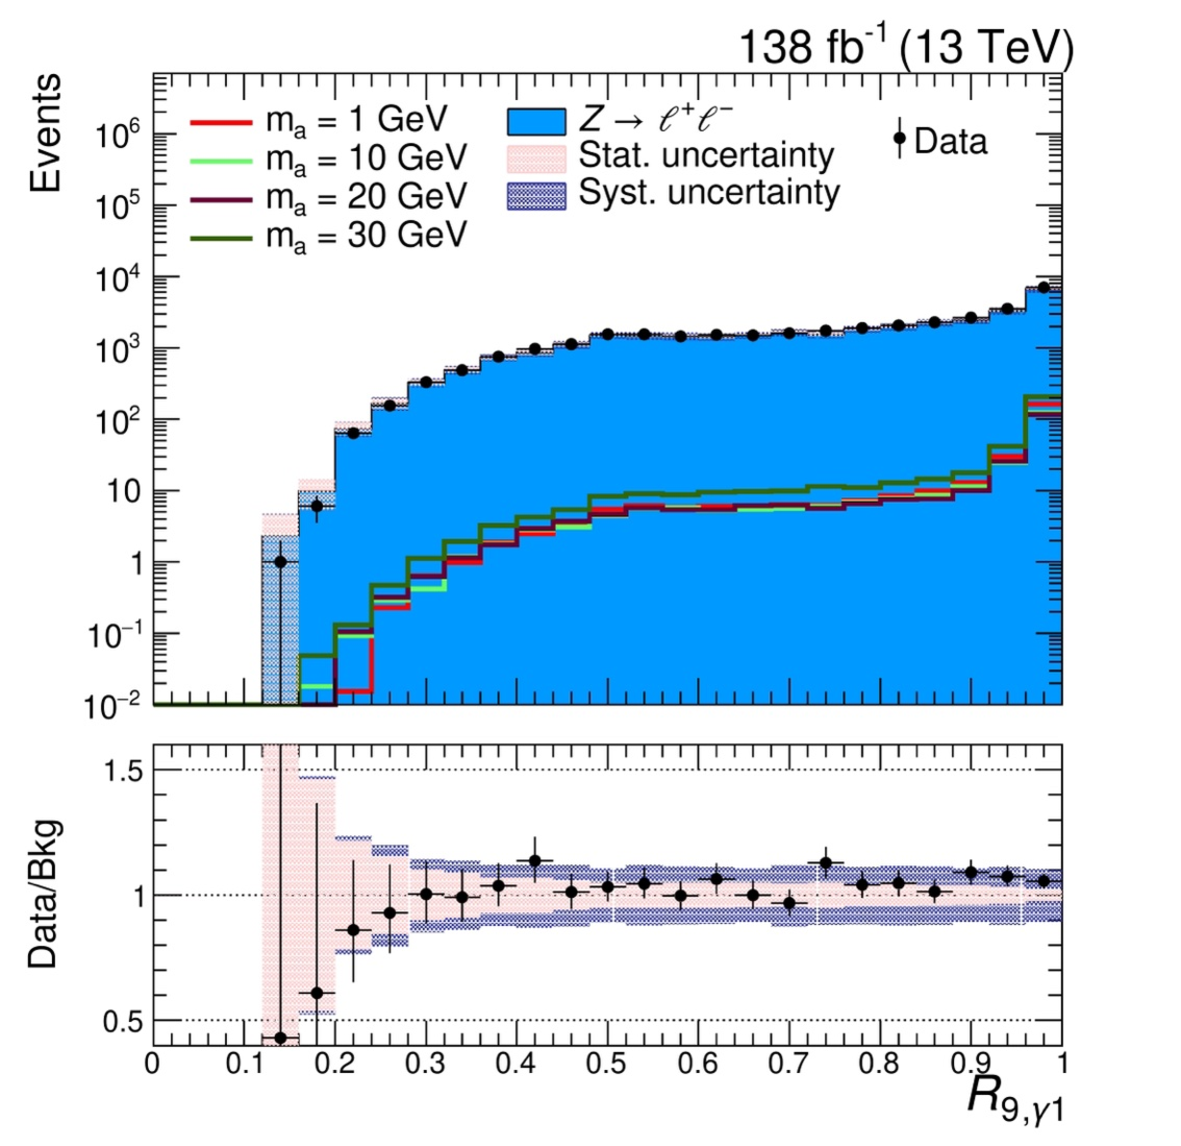
\includegraphics[width=0.42\textwidth]{figures/chapter04/BDT_input/pho1R9_log.pdf}
		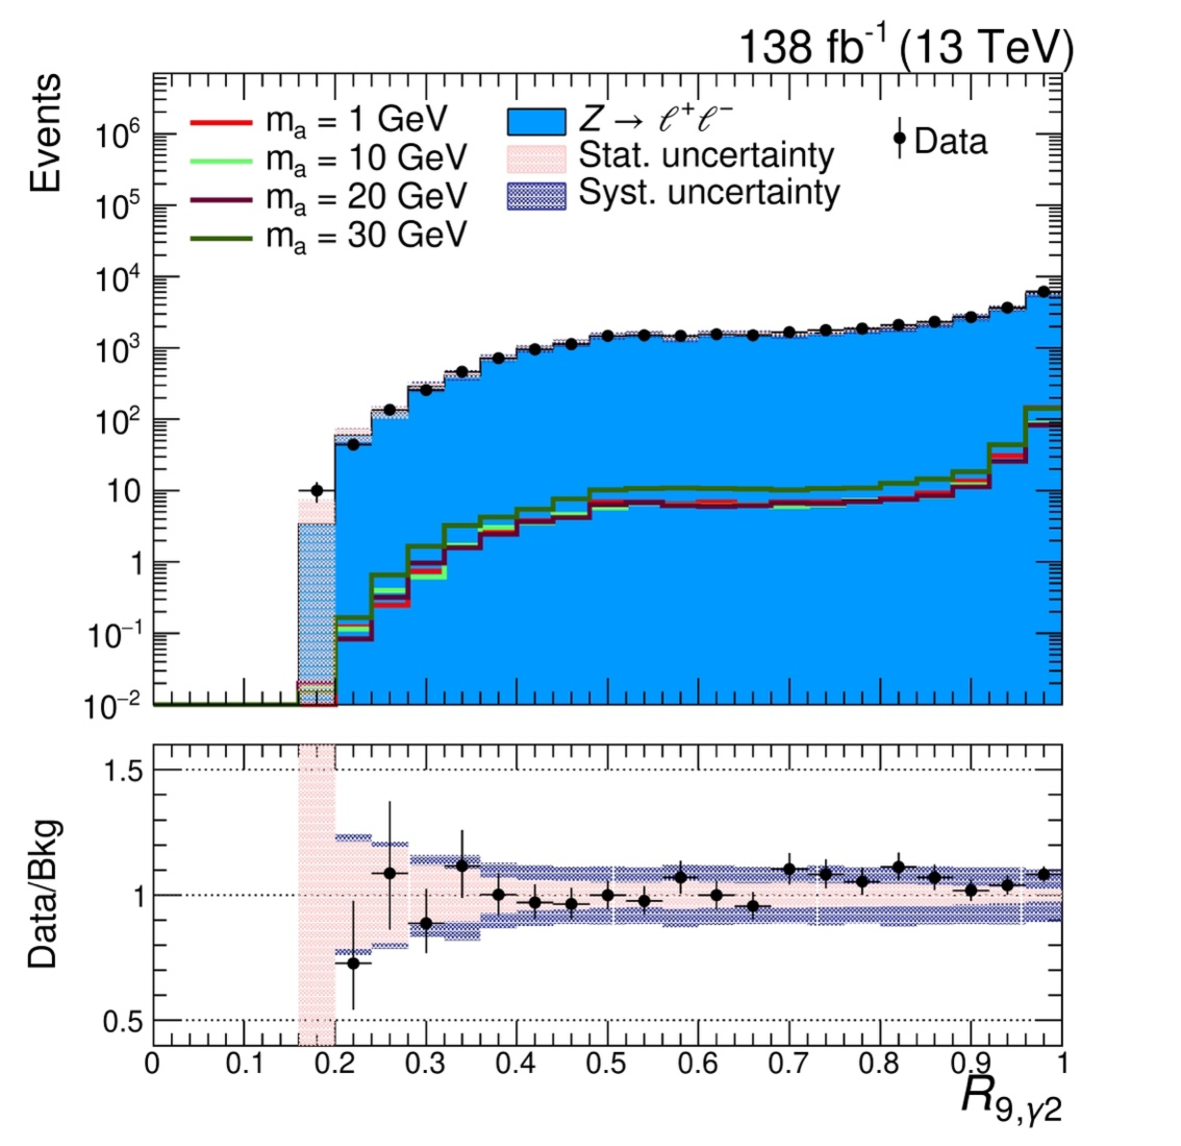
\includegraphics[width=0.42\textwidth]{figures/chapter04/BDT_input/pho2R9_log.pdf}\\
		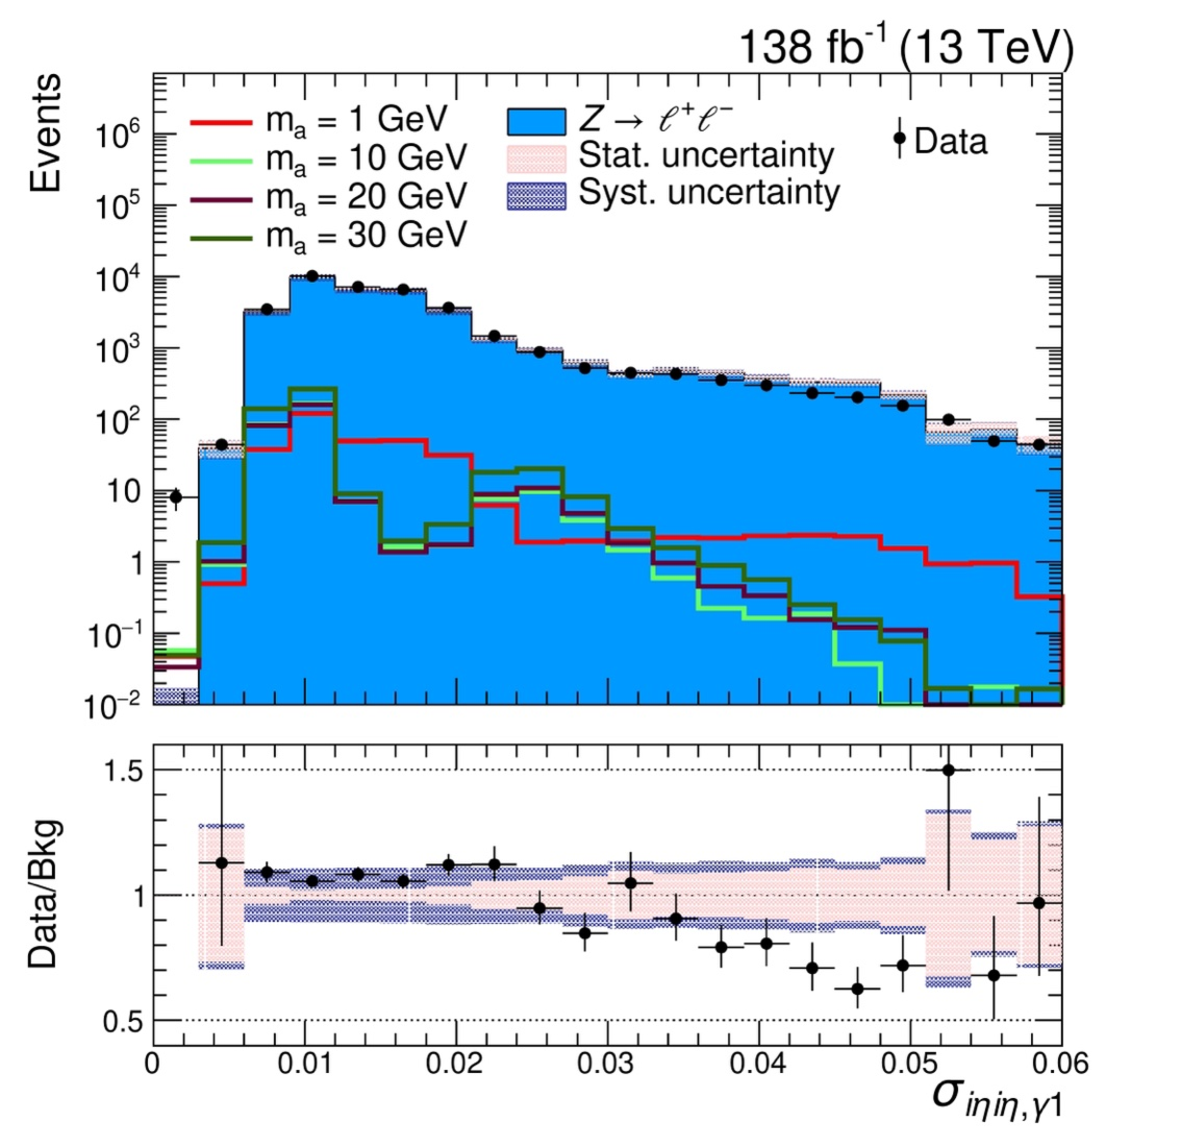
\includegraphics[width=0.42\textwidth]{figures/chapter04/BDT_input/pho1IetaIeta55_log.pdf}
		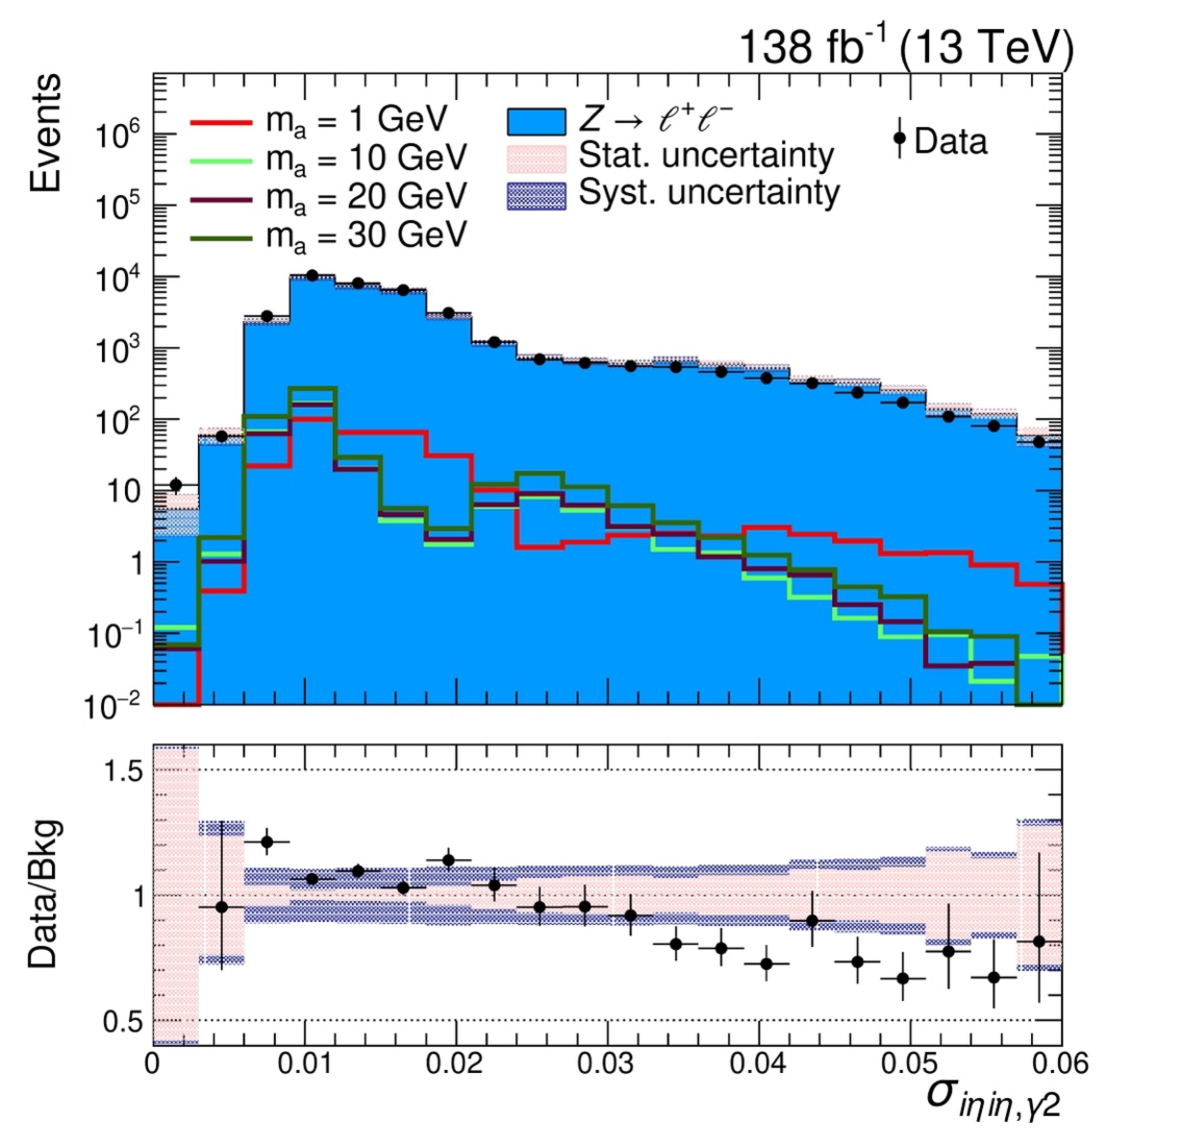
\includegraphics[width=0.42\textwidth]{figures/chapter04/BDT_input/pho2IetaIeta55_log.pdf}
    \bicaption{\quad \centering 输入变量$p_{T,\gamma1}$(左上)、$p_{T,\gamma2}$(右上)、$R_{9,\gamma1}$(左中)、$R_{9,\gamma2}$(右中)、$\sigma_{i\eta i\eta,\gamma1}$(左下)、$\sigma_{i\eta i\eta,\gamma2}$(右下)的数据和蒙卡的分布}{\quad \centering The data-MC distributions for the input variables: $p_{T,\gamma1}$ (top left), $p_{T,\gamma2}$ (top right), $R_{9,\gamma1}$ (middle left), $R_{9,\gamma2}$ (middle right), $\sigma_{i\eta i\eta,\gamma1}$ (bottom left), $\sigma_{i\eta i\eta,\gamma2}$ (bottom right)}
    \label{fig:BDT_Vars1}
\end{center}
\end{figure}

\begin{figure}[htbp]
  \begin{center}
		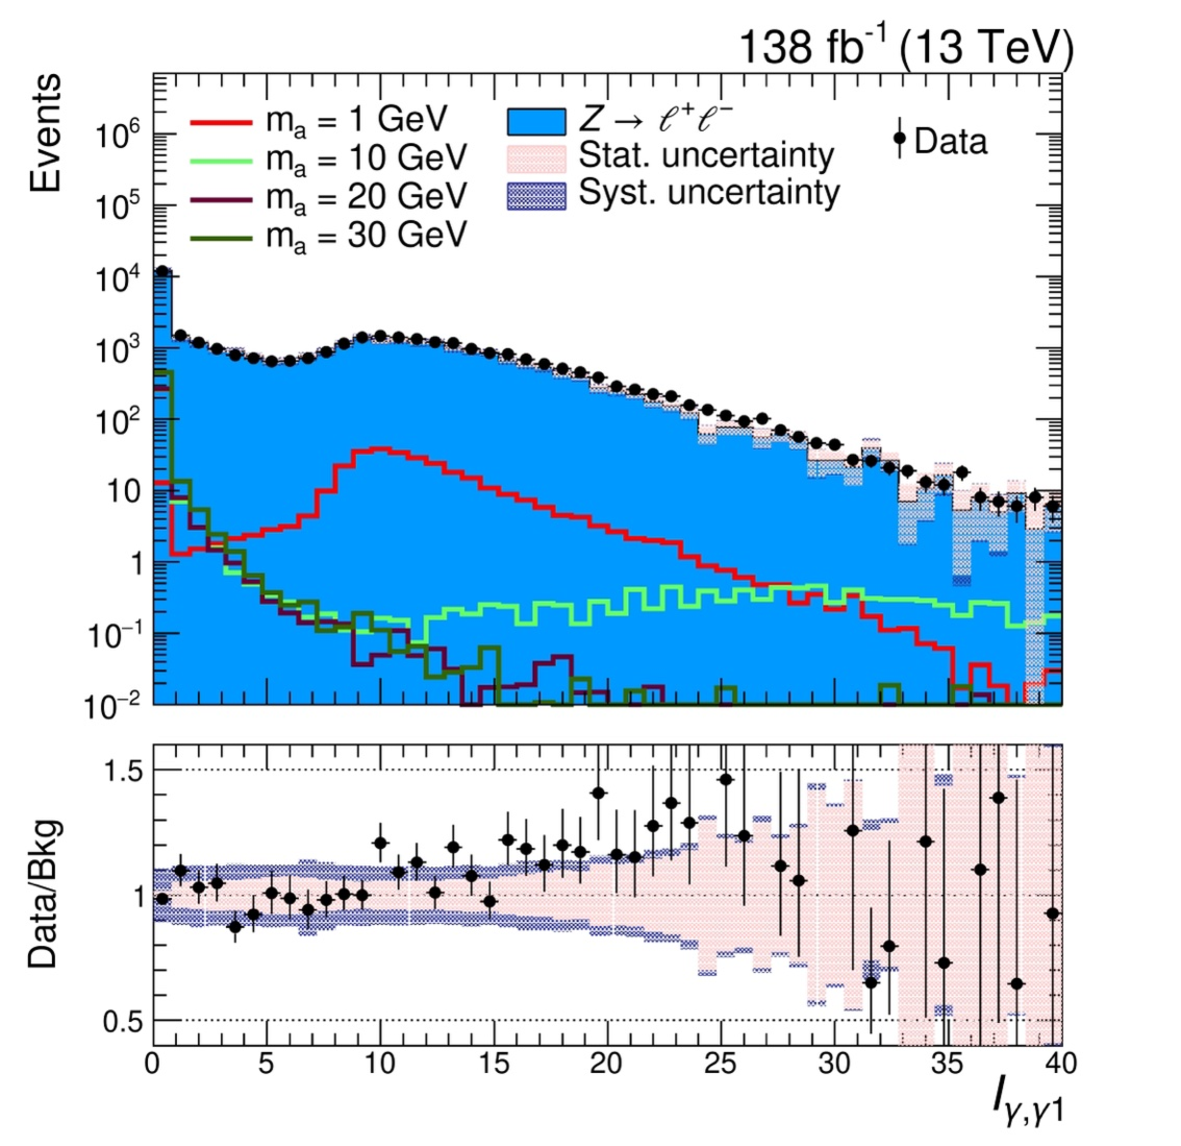
\includegraphics[width=0.42\textwidth]{figures/chapter04/BDT_input/pho1PIso_noCorr_log.pdf}
        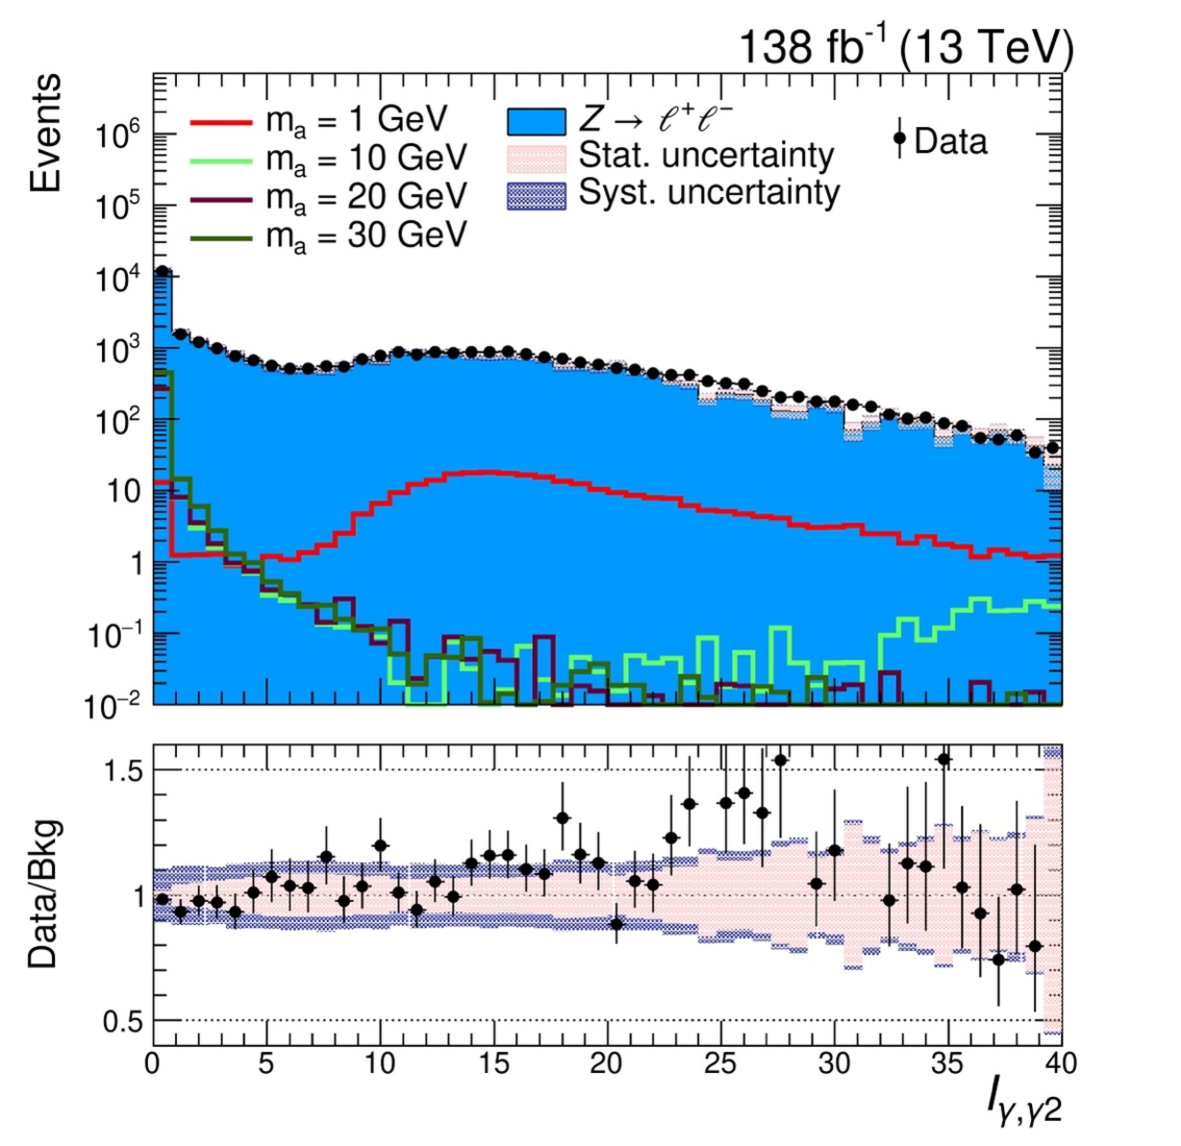
\includegraphics[width=0.42\textwidth]{figures/chapter04/BDT_input/pho2PIso_noCorr_log.pdf} \\
		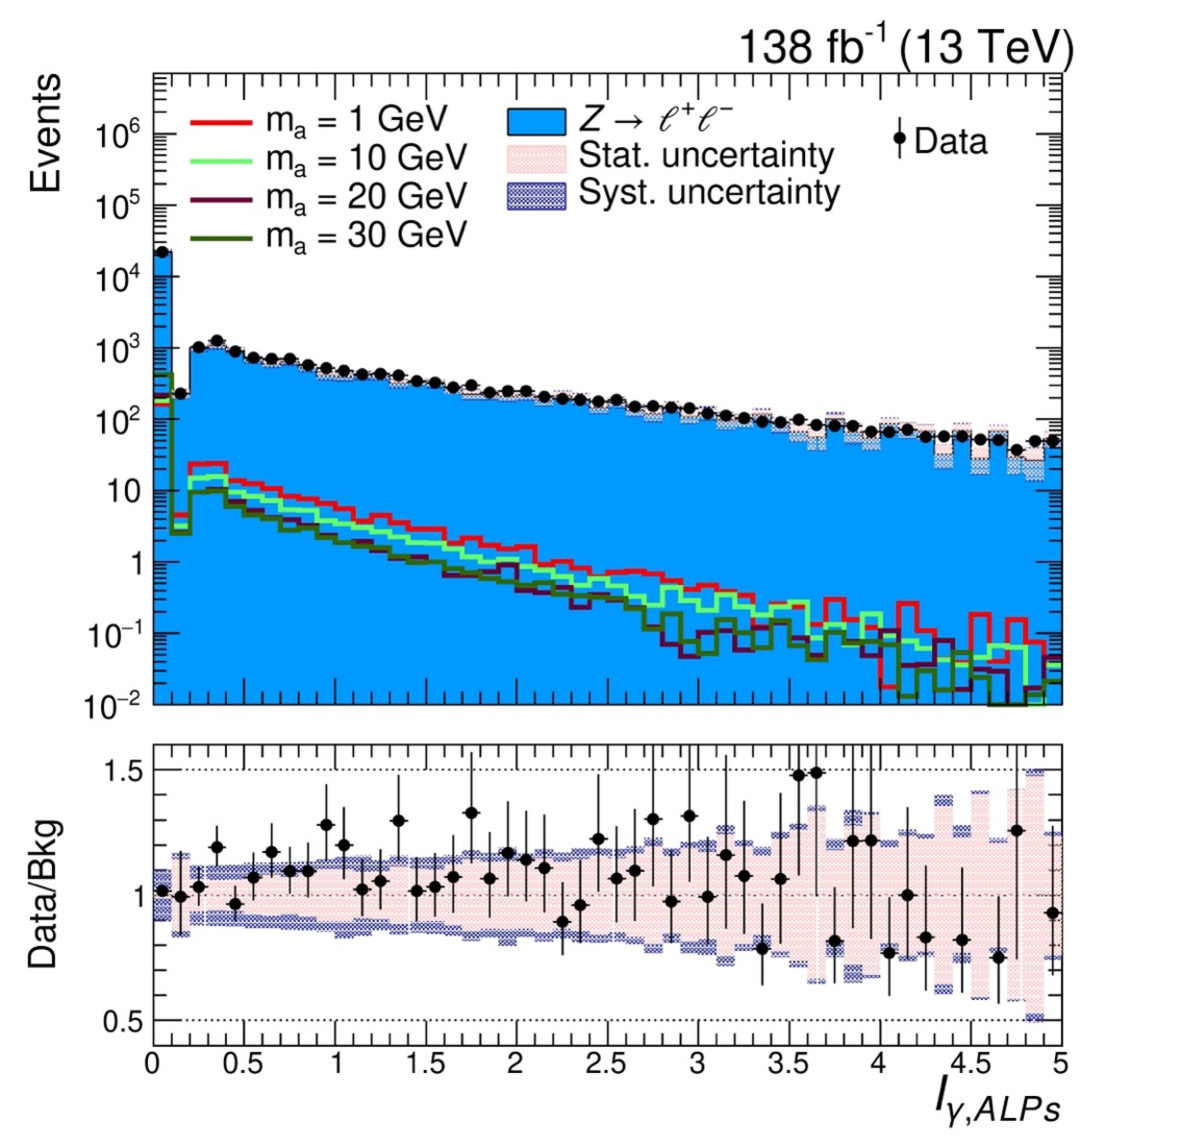
\includegraphics[width=0.42\textwidth]{figures/chapter04/BDT_input/ALP_calculatedPhotonIso_log.pdf}
		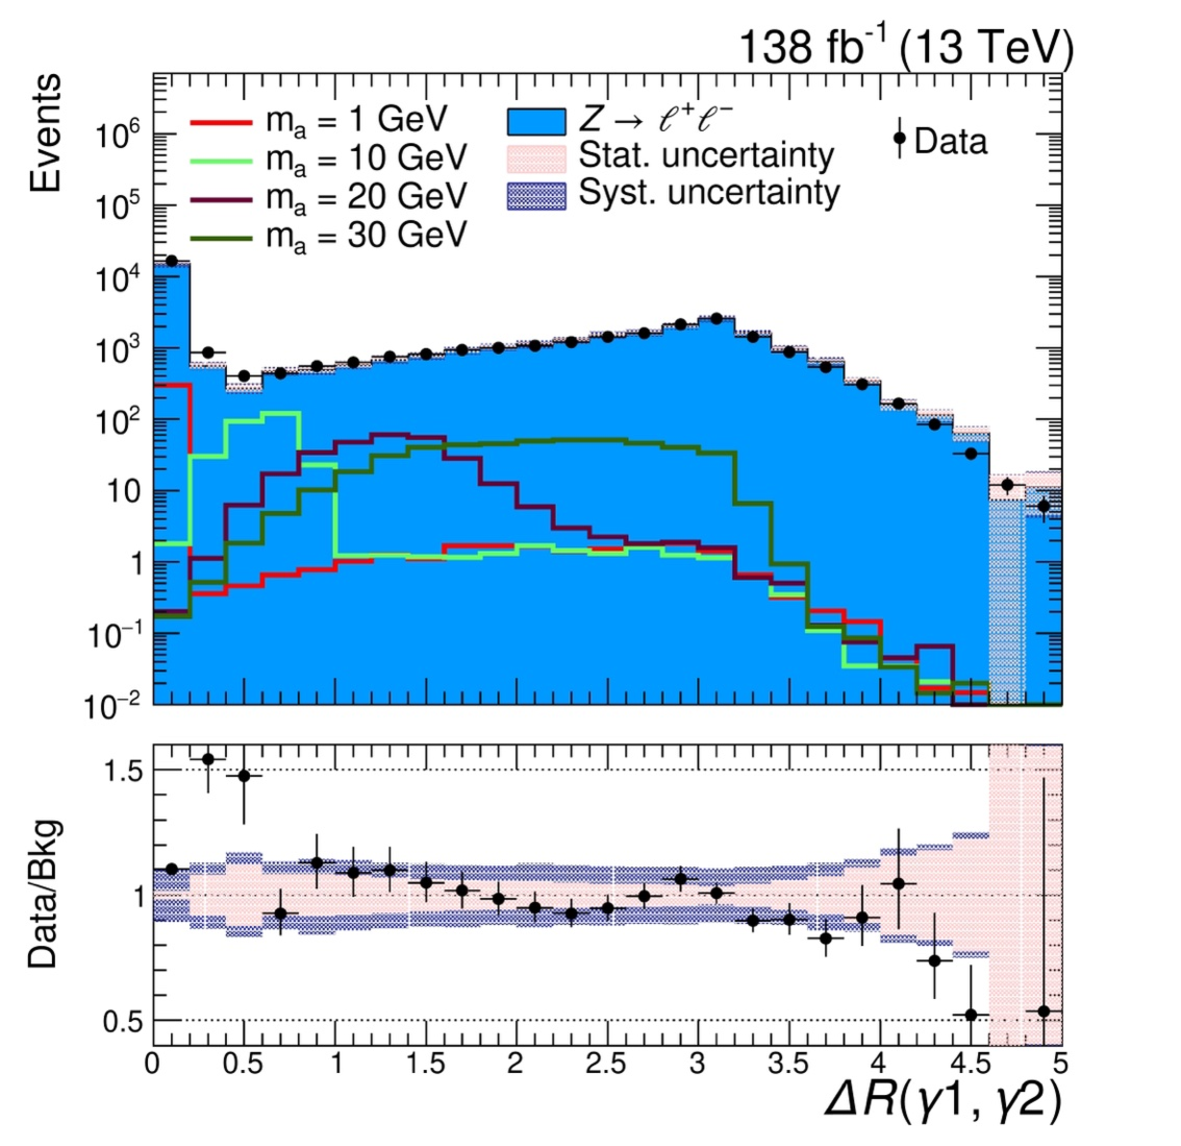
\includegraphics[width=0.42\textwidth]{figures/chapter04/BDT_input/var_dR_g1g2_log.pdf}\\
		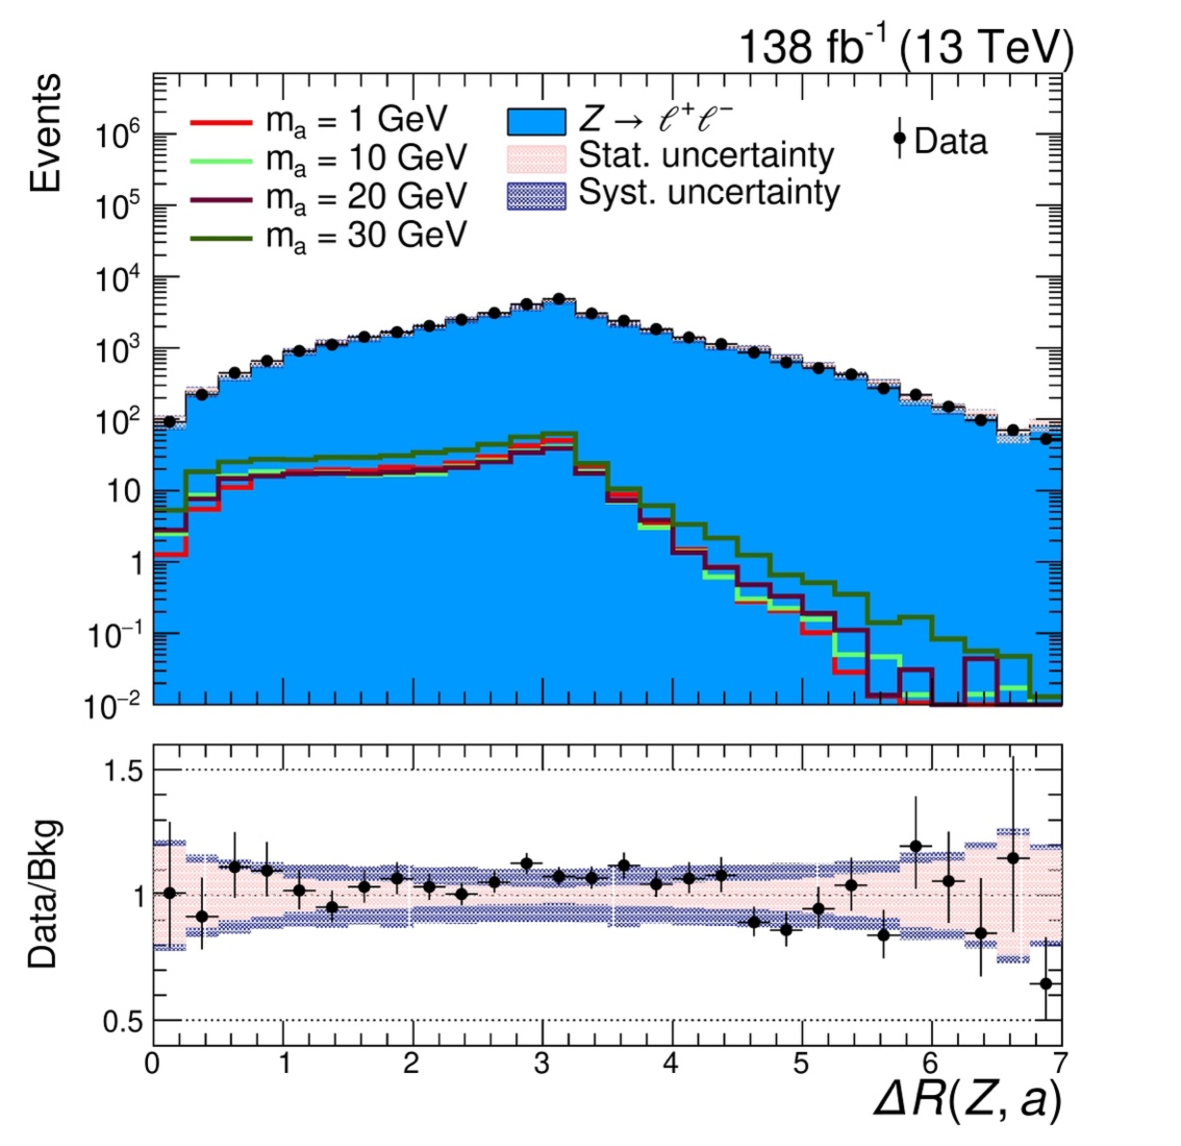
\includegraphics[width=0.42\textwidth]{figures/chapter04/BDT_input/var_dR_Za_log.pdf}
		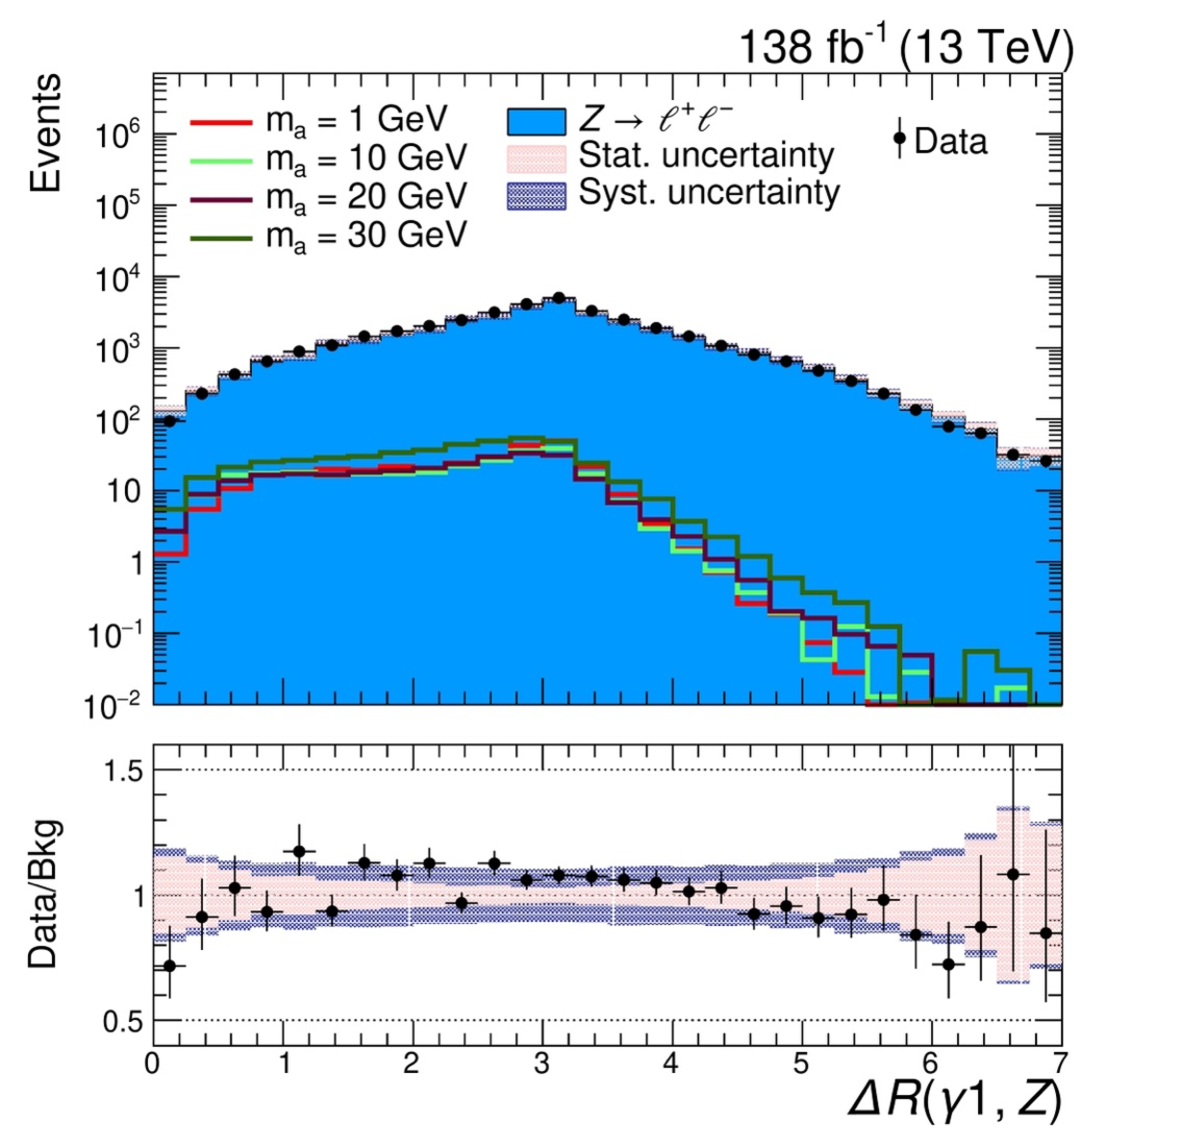
\includegraphics[width=0.42\textwidth]{figures/chapter04/BDT_input/var_dR_g1Z_log.pdf}\\
    \bicaption{\quad \centering 输入变量$I_{\gamma,\gamma1}$(左上)、$I_{\gamma,\gamma2}$(右上)、$I_{\gamma,ALPs}$(左中)、$\Delta R(\gamma1,\gamma1)$(右中)、$\Delta R(Z,a)$(左下)、$\Delta R (\gamma1,Z)$(右下)的数据和蒙卡的分布}{\quad \centering The data-MC distributions for the input variables: $I_{\gamma,\gamma1}$(top left), $I_{\gamma,\gamma2}$ (top right), $I_{\gamma,ALPs}$ (middle left), $\Delta R(\gamma1,\gamma1)$ (middle right), $\Delta R(Z,a)$ (bottom left), $\Delta R (\gamma1,Z)$ (bottom right)}
    \label{fig:BDT_Vars2}
\end{center}
\end{figure}

\begin{figure}[htbp]
  \begin{center}
		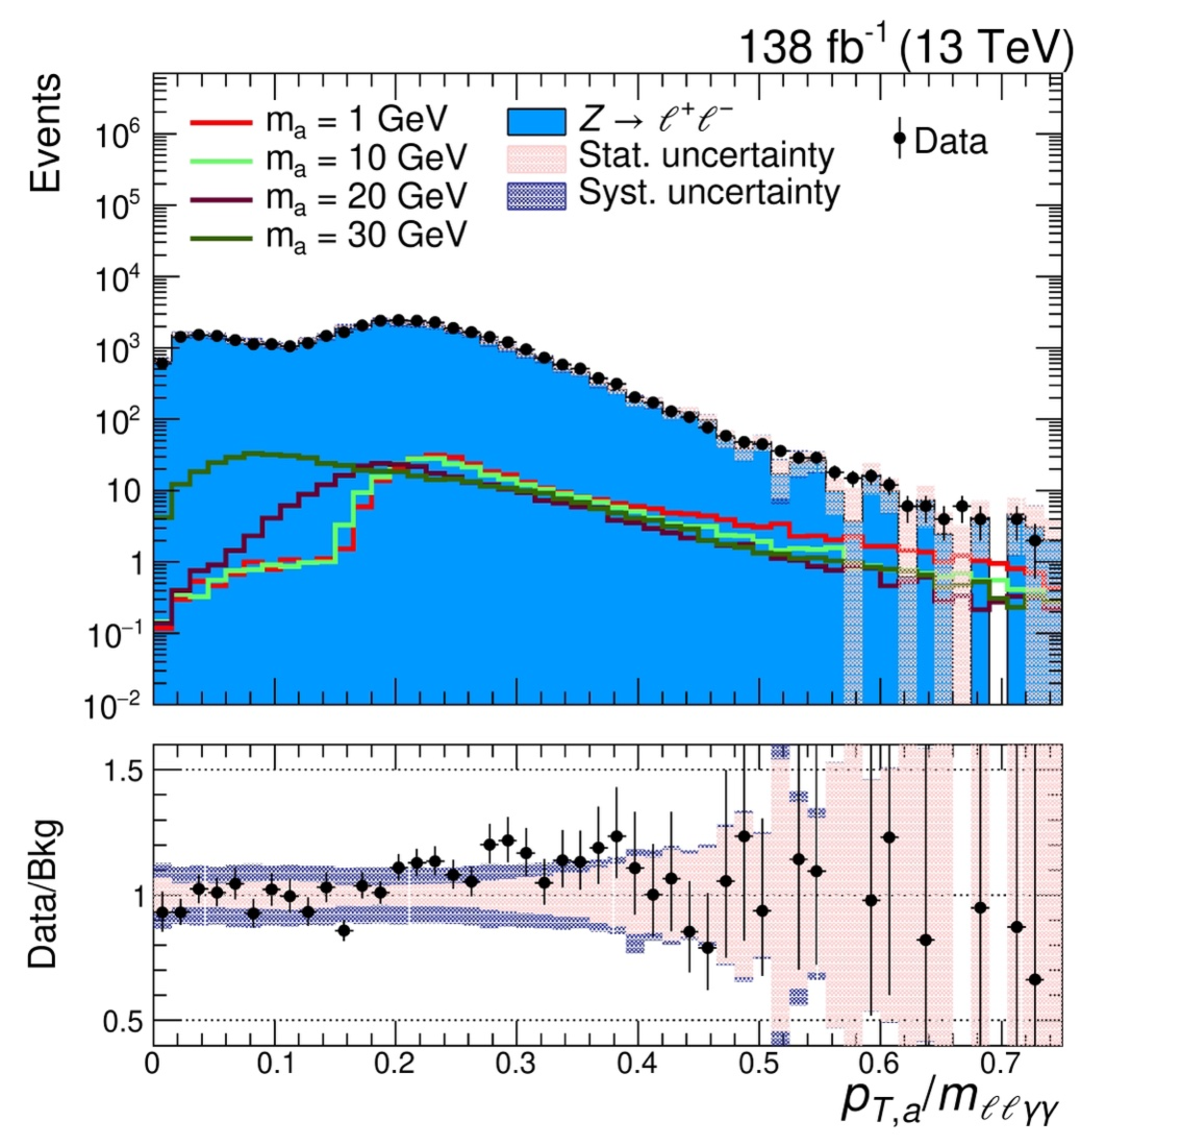
\includegraphics[width=0.42\textwidth]{figures/chapter04/BDT_input/var_PtaOverMh_log.pdf}
        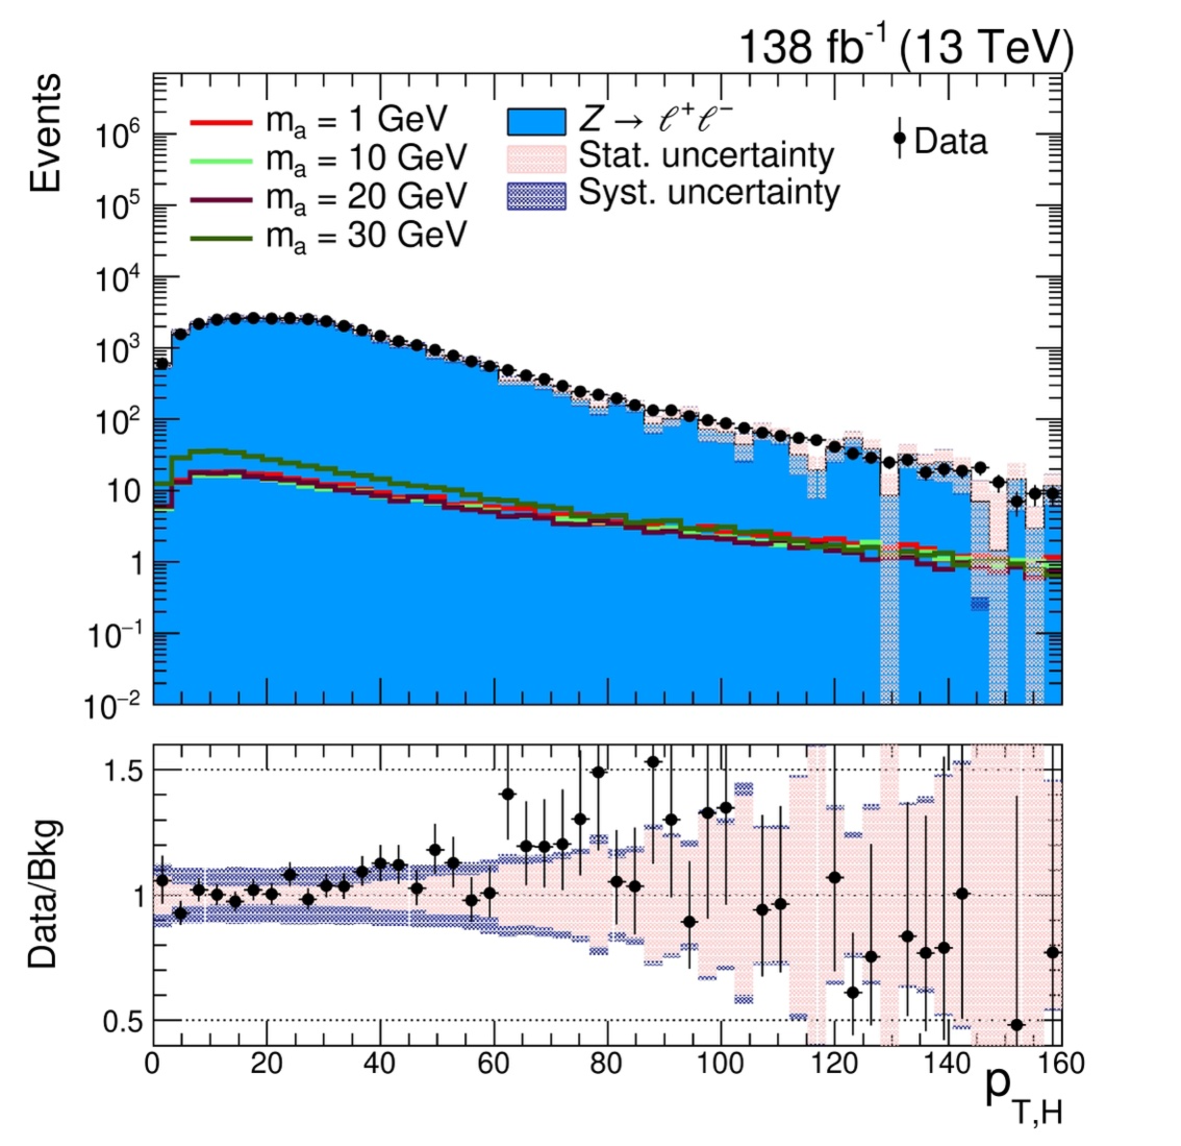
\includegraphics[width=0.42\textwidth]{figures/chapter04/BDT_input/H_pt_log.pdf} \\
    \bicaption{\quad \centering 输入变量$p_{T,a}/m_{\ell\ell\gamma\gamma}$(左图)、$p_{T,H}$(右图)的数据和蒙卡的分布}{\quad \centering The data-MC distributions for the input variables: $p_{T,a}/m_{\ell\ell\gamma\gamma}$(left), $p_{T,H}$ (right)}
    \label{fig:BDT_Vars3}
\end{center}
\end{figure}

\begin{figure}[htbp]
  \begin{center}
		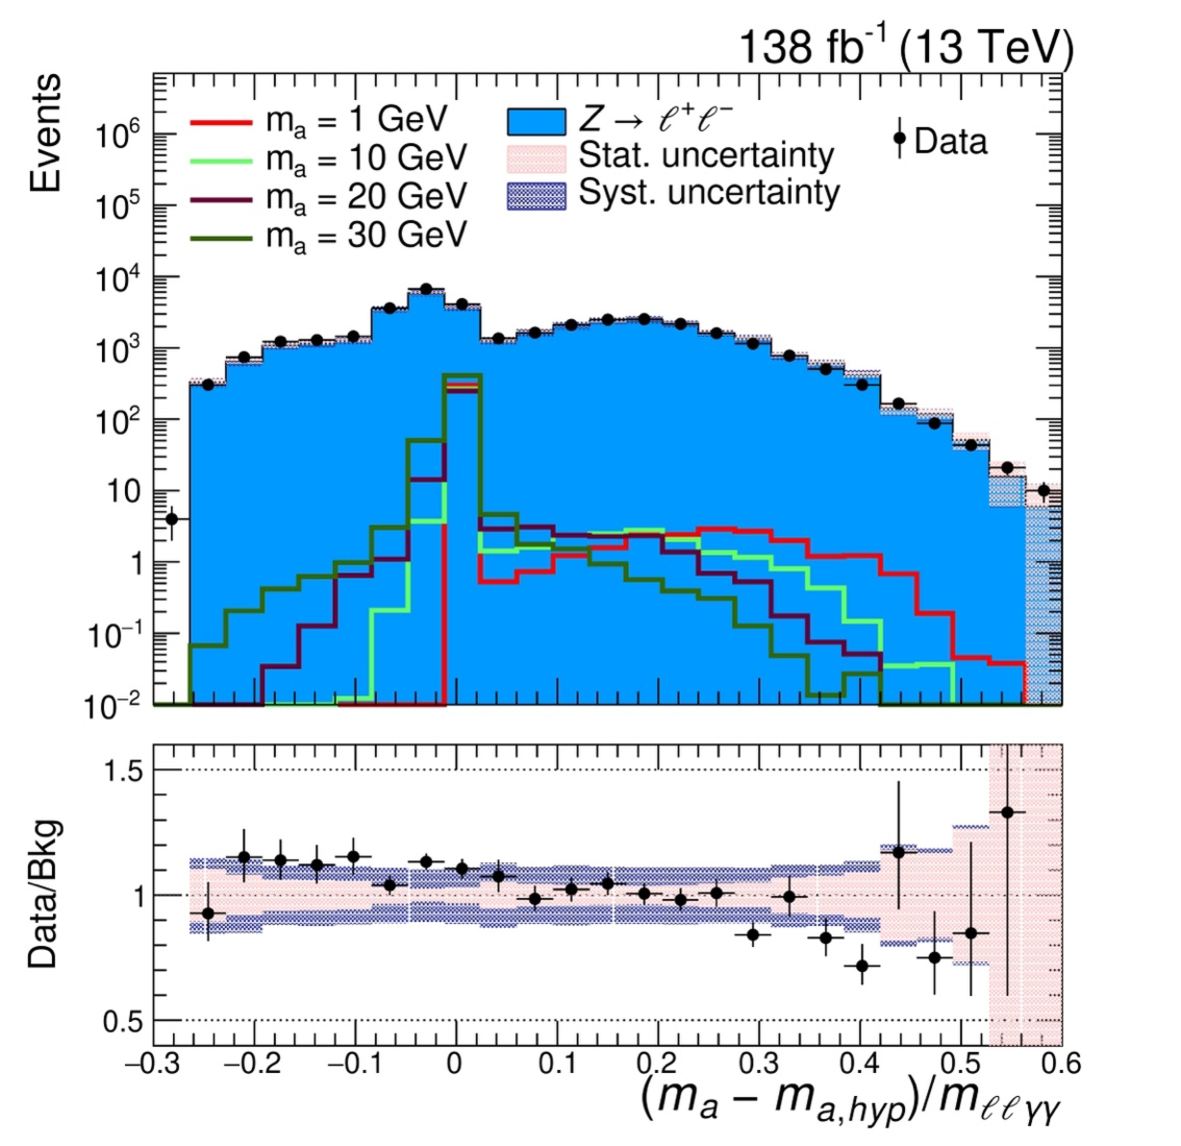
\includegraphics[width=0.6\textwidth]{figures/chapter04/BDT_input/param_log.pdf}
    \bicaption{\quad \centering 输入变量$(\ma-\mhyp)/\mllgg$的数据和蒙卡的分布}{\quad \centering The data-MC distributions for the input variable: $(\ma-\mhyp)/\mllgg$}
    \label{fig:BDT_Vars4}
\end{center}
\end{figure}

除了以上变量外,为了使得分类器的输出对整个$m_a$的范围都具有均匀且灵敏的性质,本分析使用了参数化的决策树林法~\cite{Baldi_2016}。在这个方法中,训练所使用的样本被参数化为$m_a$的函数,一个等于假设的类轴子质量的参数$\mhyp$被用作训练的输入变量,具体定义如下:
\begin{itemize}
    \item 重建出来的类轴子质量和假设的类轴子质量之间的差值和Higgs候选体质量的比值:$(\ma-\mhyp)/\mllgg$。
\end{itemize}
图~\ref{fig:BDT_Vars4}展示了这个参数的分布情况。当对模型进行训练的时候,信号样本的$\mhyp$被设置成对应样本的$\ma$的值,而本底样本的$\mhyp$均匀随机的分布在所有可能的14个$\ma$质量点之间。对于模型的评估和应用,数据和蒙卡样本中的参数$\mhyp$被设置成我们所希望寻找的$\ma$的值。比如,我们想要对5$\GeV$的类轴子进行寻找,数据和蒙卡样本中的参数$\mhyp$被固定为5,而后对提升决策树的输出进行筛选得到对应于5$\GeV$的数据和本底分布,并应用于最终的信号提取。


\subsection{模型训练}

在训练提升决策树的时候,所有的信号和本底样本都归一化到了整个Run2运行过程中的积分亮度。同时为了提高统计量,信号和本底三年的样本分别合并到一起用于训练。在提升决策树模型的构建中,本分析考虑了以下参数:
\begin{itemize}
    \item n\_estimators:决策树林的个数;
    \item max\_depth:每棵决策树的最大深度;
    \item learning\_rate:模型迭代时参数的更新步长;
    \item min\_child\_weight:最小子叶节点样本权重和,如果在此节点权重小于这个值,则停止分裂,从而有效的防止过拟合。
\end{itemize}

在训练的过程中,为了使得训练结果最优化,本分析在以上参数的参数空间进行了扫描训练,评判标准是验证样本集的接收者操作特征曲线下的面积(ROC AUC),这个参数可以用来评判模型训练的好坏,AUC的值越高表明模型训练的越好。其中,验证样本集是由训练样本集通过使用软件包scikit-learn~\cite{scikit-learn}中的交叉验证工具所得到的。为了找到具有最优性能的可能参数组合,本分析使用了GridSearchCV的方法~\cite{gridcv}。在此方法中,具有不同参数组合的提升决策树被用于训练并比较它们之间的性能差异,即AUC的值。在每一个参数格点上,提升决策树的训练使用了交叉验证的方法,主要步骤包括:
\begin{itemize}
    \item 将样本平均分为k部分;
    \item 将其中的k-1个部分用于训练模型,剩下的一个部分用于验证模型,并重复这个步骤遍历样本的所有部分。
\end{itemize}
而后交叉验证所得到的k个ROC AUC的值的平均值作为对应参数格点的AUC值。

本分析使用了k=2的交叉验证方法,对参数空间的格点扫描范围在列表~\ref{tab:BDT_para_scan}中展示。其中,AUC的值在所有参数组合形式中的变化小于0.3\%,这意味着训练出来的提升决策树具有非常好的稳定性。列表~\ref{tab:BDT_para_scan}也展示了最终用于分类所使用的参数组合。

训练过程中各个输入变量对模型的重要性(Importance)可以使用基尼指数(Gini index)错误率作为评价指标来衡量,其直观意义表示某一提升决策树节点中某一特征类别标记不一致的概率。某一特征在特定节点的重要性可以定义为该节点的基尼指数和分枝后的两个新节点的基尼指数之差,而后将所有节点的重要性相加并对所有特征进行归一化处理,可以得到训练过程中各个输入变量对模型的重要性,结果如图~\ref{fig:BDT_rank}所示。其中,重要性位于前四位的变量分别为$\sigma_{i\eta i\eta, \gamma 1}$、$(m_{a}-m_{a,hyp})/m_{\ell\ell\gamma\gamma}$、$\sigma_{i\eta i\eta, \gamma 2}$和$R_{9, \gamma 1}$,主要原因是本底过程中的假光子主要来自于将夸克和胶子产生的喷注错误的判断为光子,而相比于真正的光子,这些假光子在簇射过程中会在喷注中产生更多的次级粒子,从而使得喷注的$\sigma_{i\eta i\eta}$偏大、$R_9$偏小,因此这两个变量可以用来非常好的辨别真假光子。而对于变量$(m_{a}-m_{a,hyp})/m_{\ell\ell\gamma\gamma}$,由于其使用了双光子的不变质量信息,重建出的$m_a$主要分布在$\mhyp$附近,使得该变量对于信号样本只能集中分布在0附近,而对于本底样本,不同的动力学性质使得该变量可能位于偏离0的位置,因此具有非常好的信号本底识别度。

\begin{table}[h]
  \begin{center}
  \bicaption{\quad \centering 为寻找最优参数选项所执行的扫描列表以及用于最终分类的参数}{\quad \centering List of scans performed to look for the best parameters option, and the parameters used for the final categorization}
    \begin{tabular}{ccccc} \hline
       \multicolumn{4}{c} {Parameter Grid} & Option \\ \hline
       n\_estimators & max\_depth & learning\_rate & min\_child\_weight & AUC \\ \hline
       500 & 3 & 0.05 & 5 & $0.9878$\\
       1000 & 4 & 0.1 & & $\backsim$\\
       1500 & 5 & 0.15 & & $0.9907$\\ \hline
       \multicolumn{5}{c} {Parameter used for the categorization}\\ \hline 
       1500 & 3 & 0.15 & 5 & 0.9907 \\ \hline 
    \end{tabular}
    \label{tab:BDT_para_scan}
  \end{center}
\end{table}

\begin{figure}[htbp]
  \begin{center}
		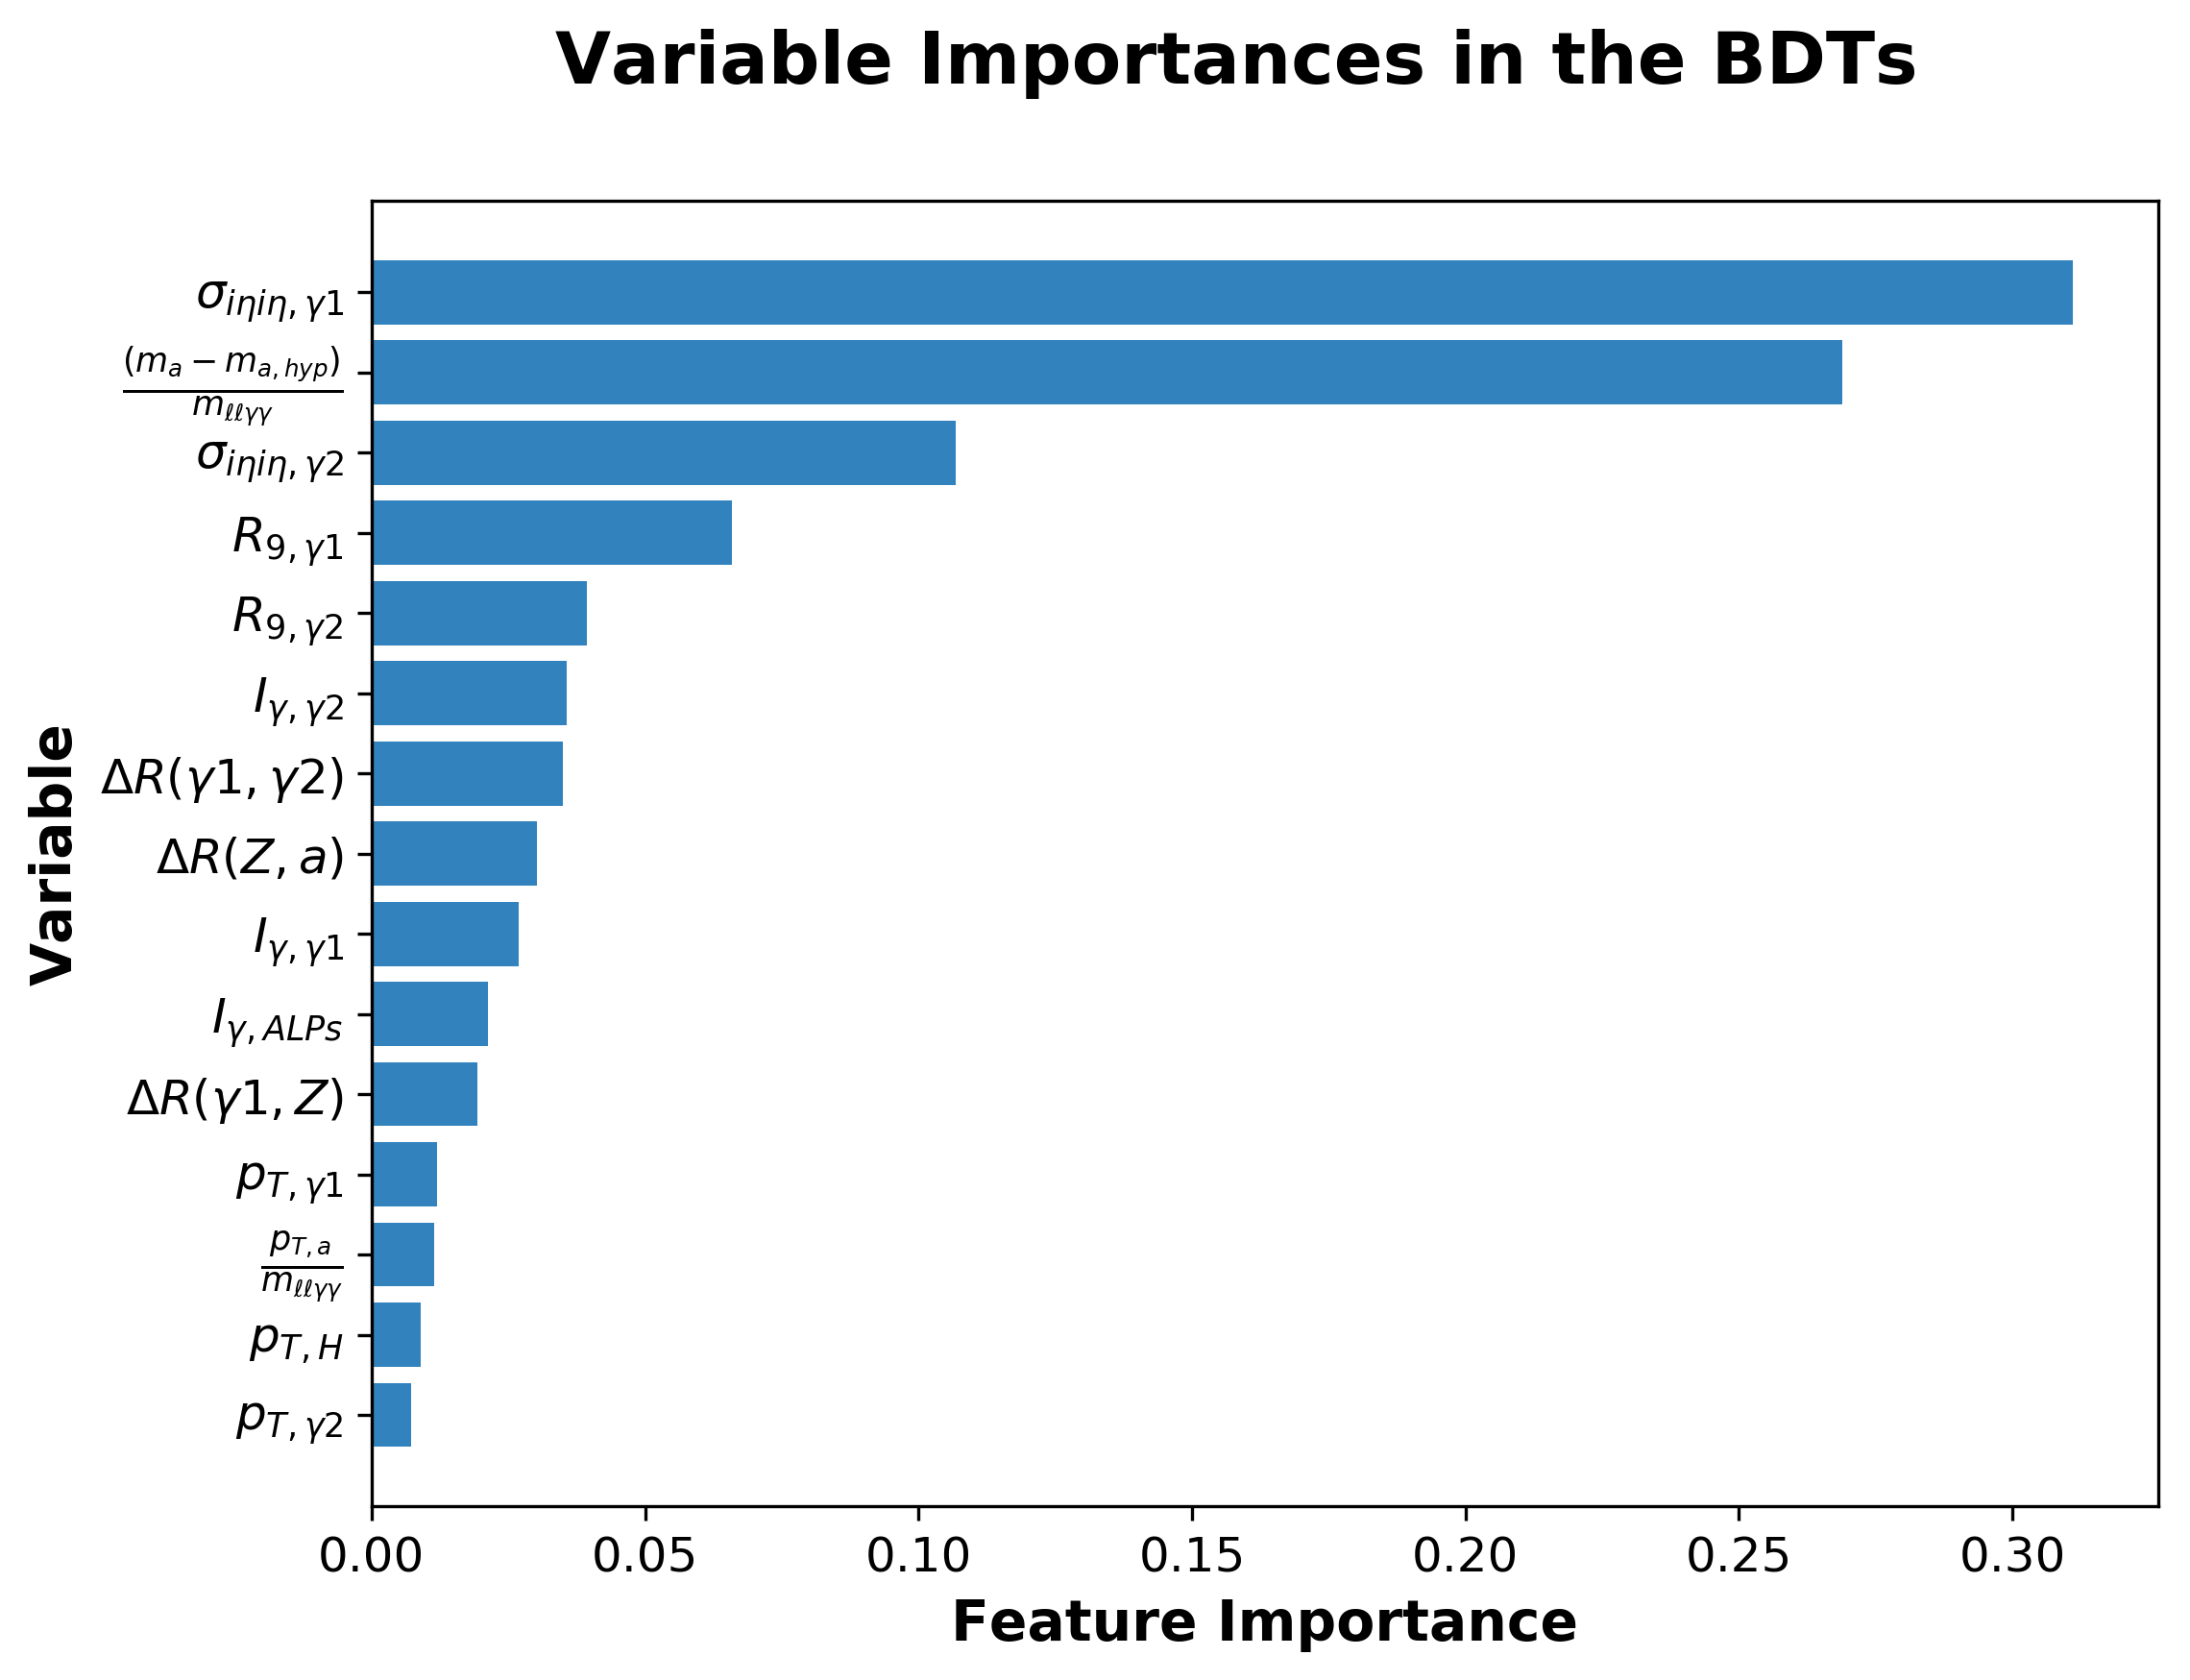
\includegraphics[width=0.6\textwidth]{figures/chapter04/BDT_score/rank.png}
    \bicaption{\quad \centering 输入变量的重要性}{\quad \centering The importance of the input variables}
    \label{fig:BDT_rank}
\end{center}
\end{figure}

\subsection{模型评估}

训练样本和评估样本的提升决策树得分分布如图~\ref{fig:BDT_evalue}所示。其中,将评估样本集通过训练模型得到的信号和本底的分布与训练样本集的分布进行K-S检验可以得到对应的p值分别为0.96和0.23,这说明对提升决策树的训练是合理的,没有发生过拟合。通过将$\mhyp$设置为对应不同$\ma$的值,可以对不同ALPs质量点的提升决策树得分分别进行评估。因此,对于不同的ALPs质量点,可以分别得到不同的信号、数据和本底的提升决策树得分分布,如图~\ref{fig:BDT_score1}、~\ref{fig:BDT_score2}、~\ref{fig:BDT_score3}所示。

\begin{figure}[htbp]
  \begin{center}
		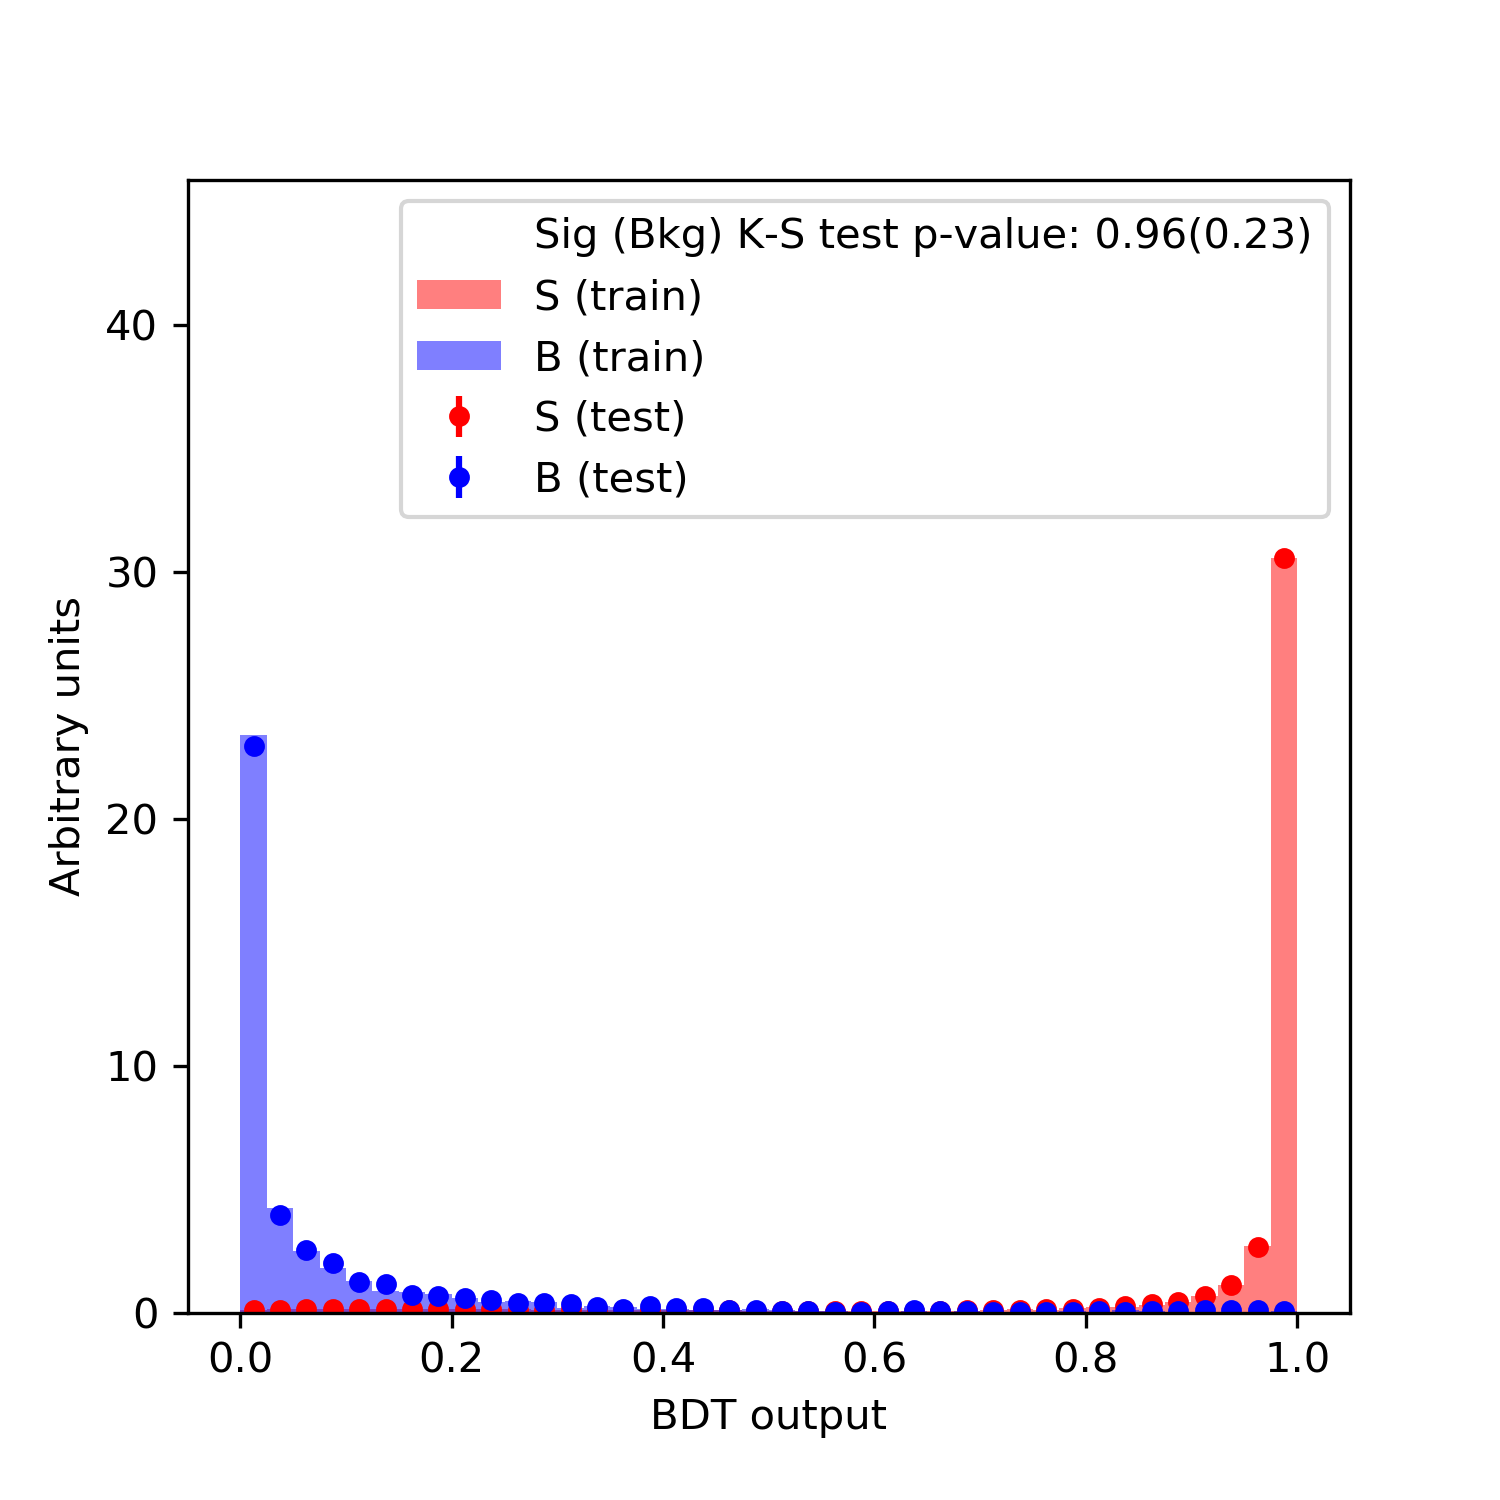
\includegraphics[width=0.52\textwidth]{figures/chapter04/BDT_score/BDT_output-2.png}
    \bicaption{\quad \centering 训练样本和评估样本的提升决策树得分分布}{\quad \centering Distributions of the BDTs score for training sample and testing sample}
    \label{fig:BDT_evalue}
\end{center}
\end{figure}

\begin{figure}[htbp]
  \begin{center}
		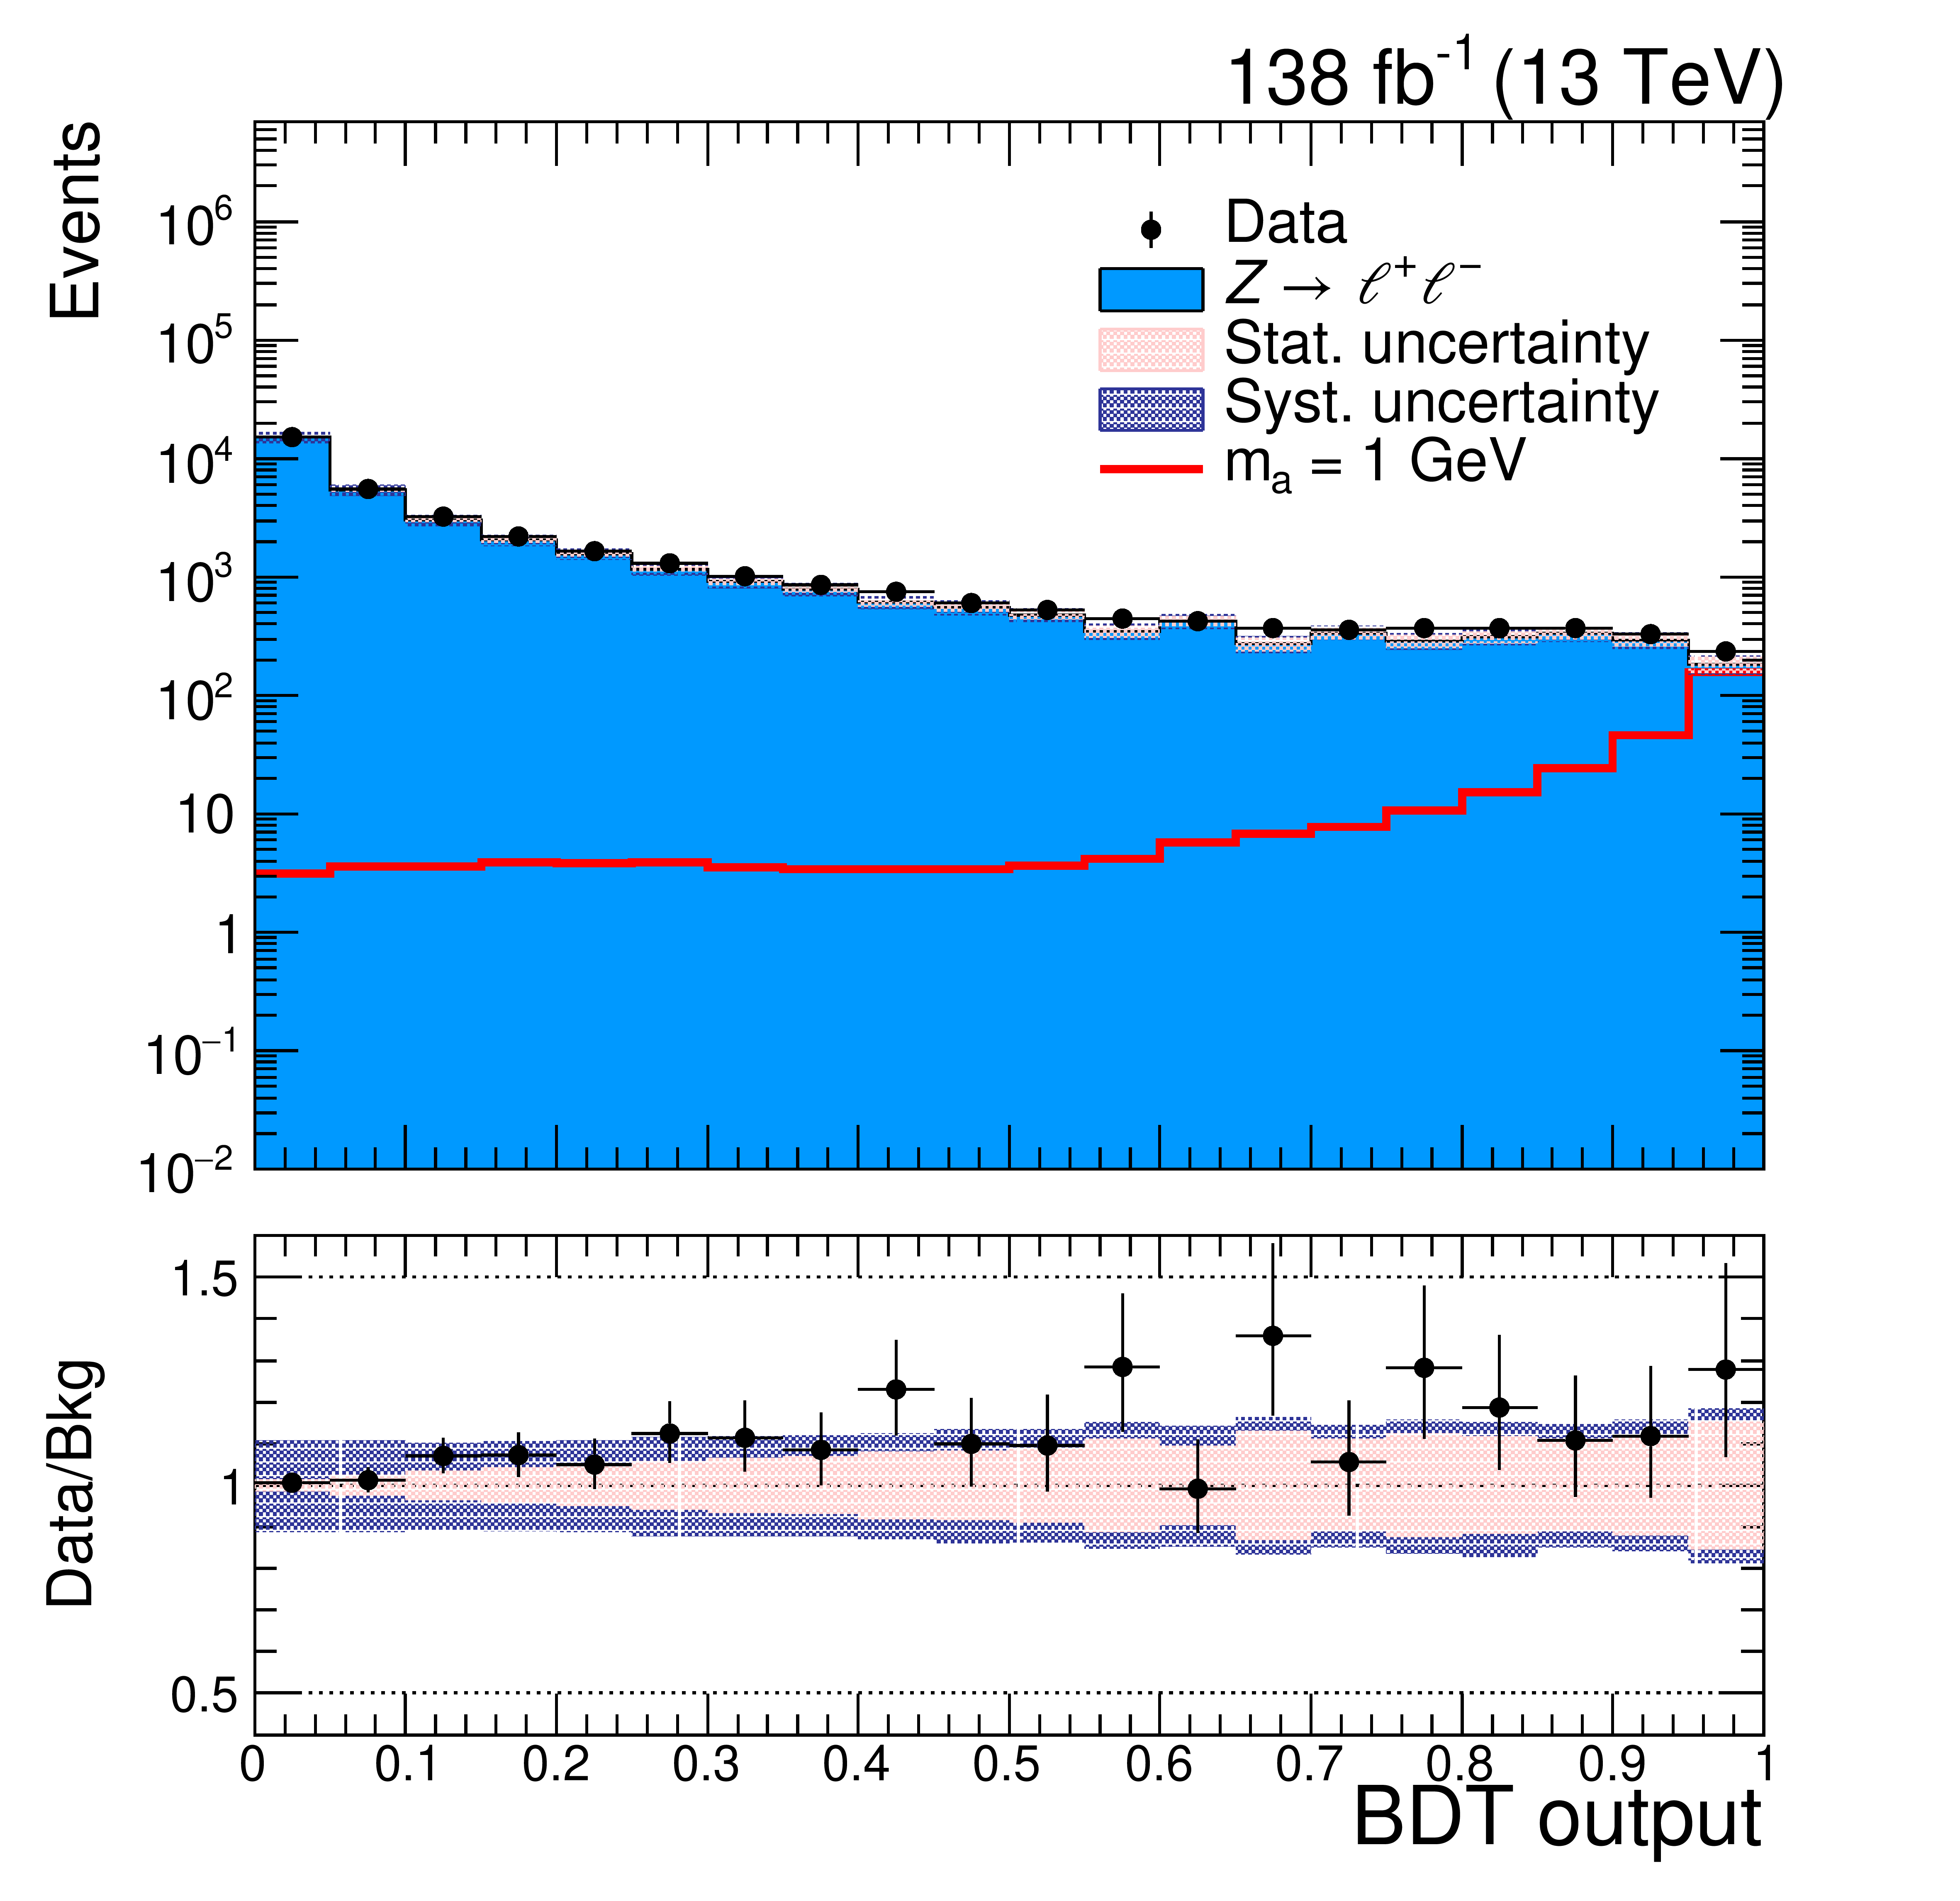
\includegraphics[width=0.42\textwidth]{figures/chapter04/BDT_score/mvaVal_M1_log.png}
        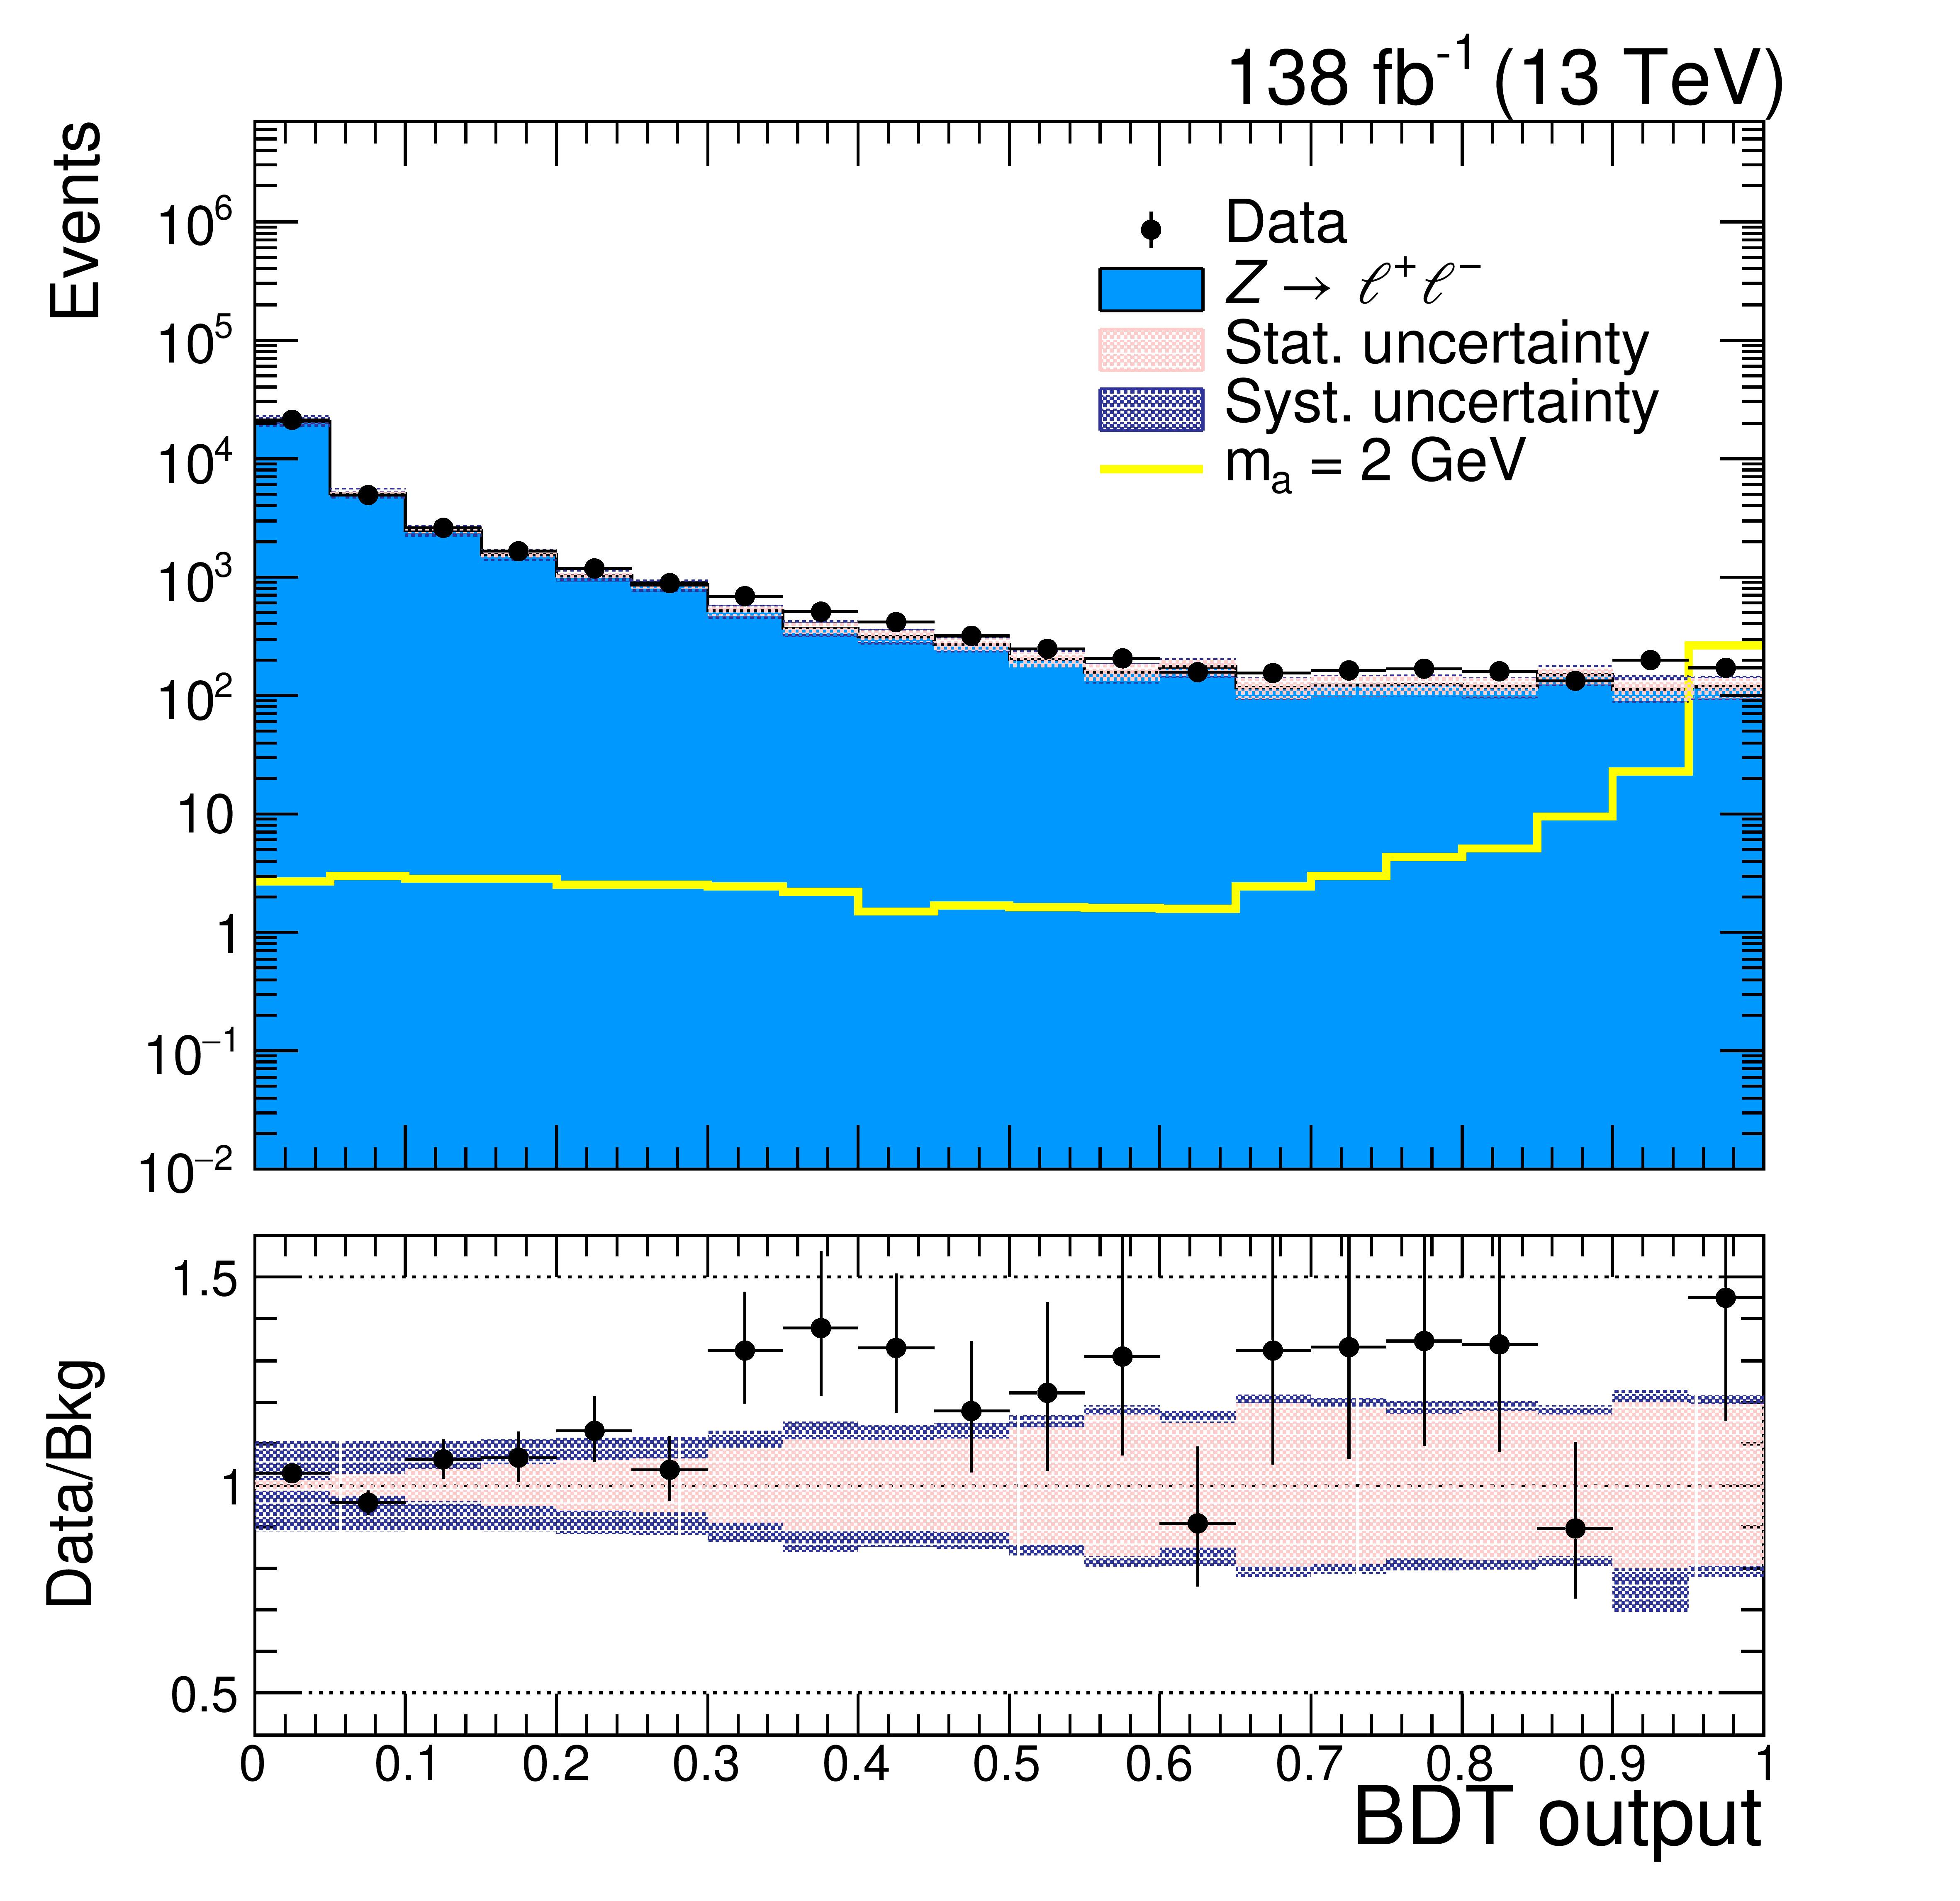
\includegraphics[width=0.42\textwidth]{figures/chapter04/BDT_score/mvaVal_M2_log.png} \\
		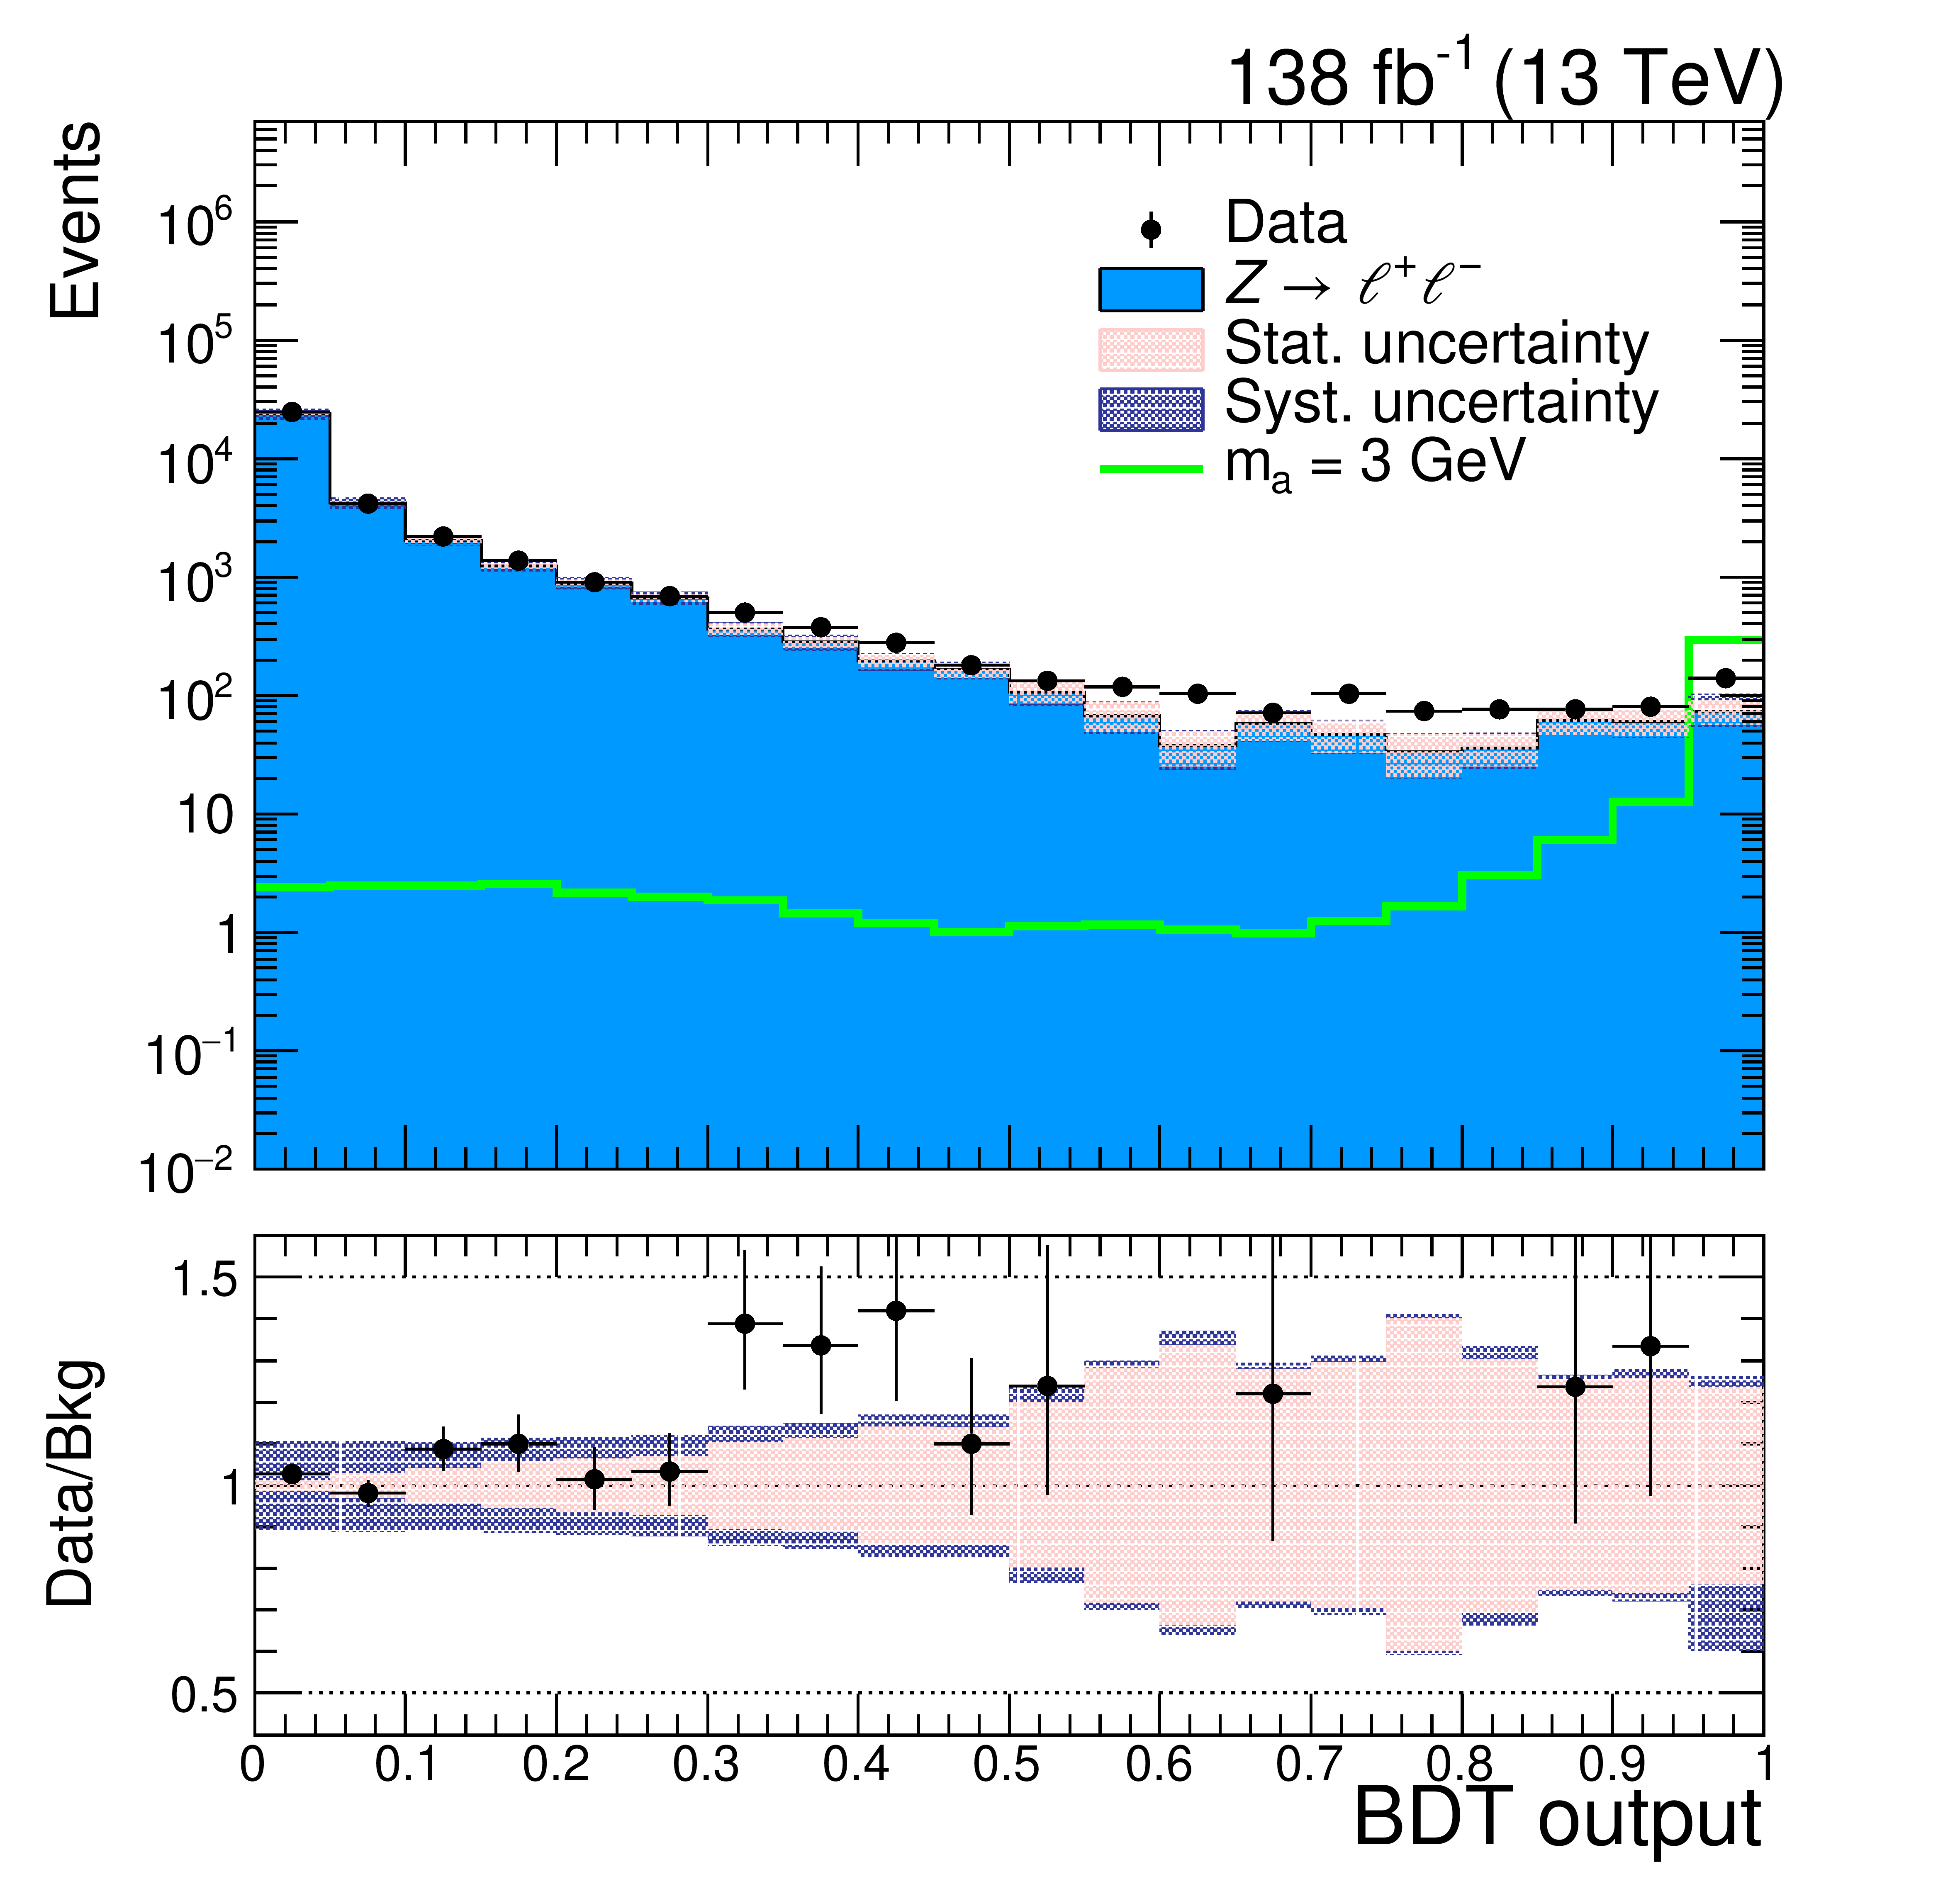
\includegraphics[width=0.42\textwidth]{figures/chapter04/BDT_score/mvaVal_M3_log.png}
		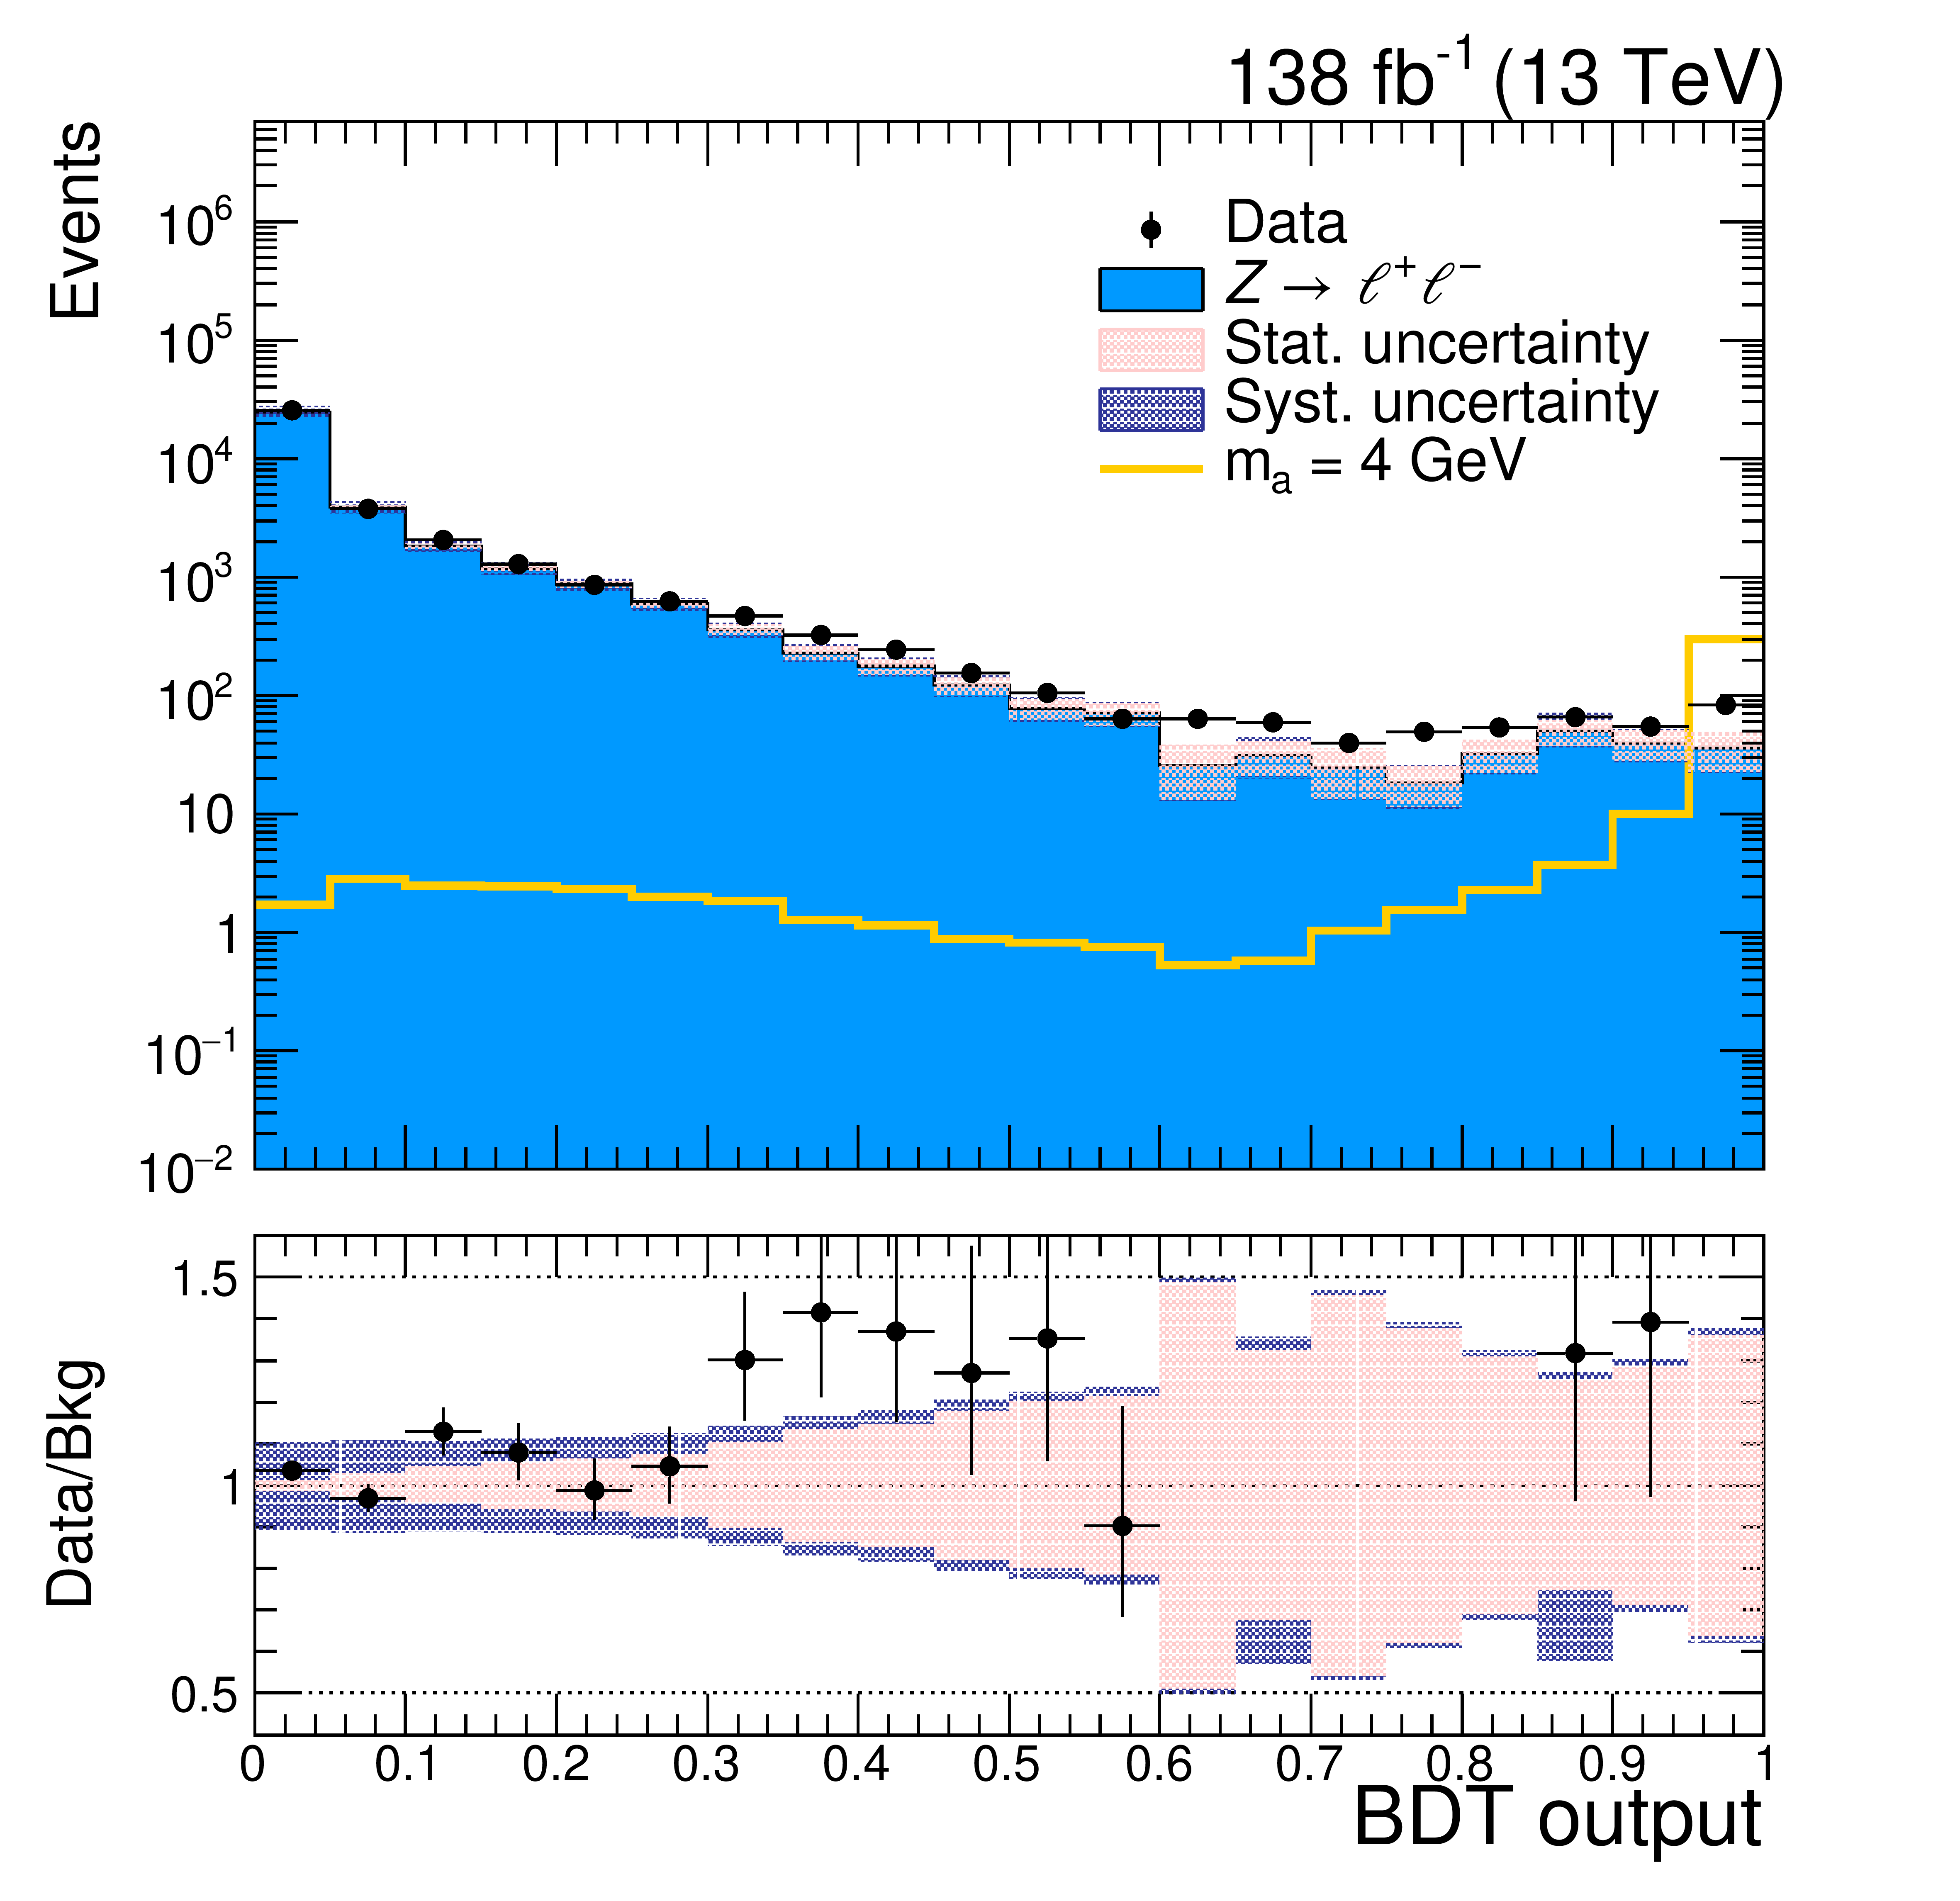
\includegraphics[width=0.42\textwidth]{figures/chapter04/BDT_score/mvaVal_M4_log.png}\\
		\includegraphics[width=0.42\textwidth]{figures/chapter04/BDT_score/mvaVal_M5_log.png}
		\includegraphics[width=0.42\textwidth]{figures/chapter04/BDT_score/mvaVal_M6_log.png}\\
    \bicaption{\quad \centering 不同ALPs质量点下的提升决策树得分分布}{\quad \centering Distributions of the BDTs score for different ALPs mass points}
    \label{fig:BDT_score1}
\end{center}
\end{figure}

\begin{figure}[htbp]
  \begin{center}
		\includegraphics[width=0.42\textwidth]{figures/chapter04/BDT_score/mvaVal_M7_log.png}
        \includegraphics[width=0.42\textwidth]{figures/chapter04/BDT_score/mvaVal_M8_log.png} \\
		\includegraphics[width=0.42\textwidth]{figures/chapter04/BDT_score/mvaVal_M9_log.png}
		\includegraphics[width=0.42\textwidth]{figures/chapter04/BDT_score/mvaVal_M10_log.png}\\
		\includegraphics[width=0.42\textwidth]{figures/chapter04/BDT_score/mvaVal_M15_log.png}
		\includegraphics[width=0.42\textwidth]{figures/chapter04/BDT_score/mvaVal_M20_log.png}\\
    \bicaption{\quad \centering 不同ALPs质量点下的提升决策树得分分布}{\quad \centering Distributions of the BDTs score for different ALPs mass points}
    \label{fig:BDT_score2}
\end{center}
\end{figure}

\begin{figure}[htbp]
  \begin{center}
		\includegraphics[width=0.42\textwidth]{figures/chapter04/BDT_score/mvaVal_M25_log.png}
        \includegraphics[width=0.42\textwidth]{figures/chapter04/BDT_score/mvaVal_M30_log.png} \\
    \bicaption{\quad \centering 不同ALPs质量点下的提升决策树得分分布}{\quad \centering Distributions of the BDTs score for different ALPs mass points}
    \label{fig:BDT_score3}
\end{center}
\end{figure}

\subsection{事例分类}

为了能够得到最高的信号显著度,本分析根据提升决策树的输出得分将所有事例分为了不同的类别,具体评判标准为使得近似平均显著度~\cite{Cowan:2010js}(Approximate Mean Significance,AMS)具有极大值。AMS的定义为:
\begin{equation}
    \textrm{AMS} = \sqrt{2((S+B)\ln{(1+\frac{S}{B})} - S)}\label{con:AMS}.
\end{equation}
其中,S和B分别表示信号区间(Signal region,SR)的信号和本底事例数,信号区间的定义为$115 <\mllgg< 135\GeV$。对于固定类别数量的分类情况,提升决策树的筛选边界条件被选为使得每个类别的AMS平方和开根号具有极大值的得分。此外,由于最终信号的提取是通过利用参数化的函数形式对数据中的$\mllgg$分布进行拟合所得到的。其中,描述本底分布的本底模型是通过利用多种解析函数对数据中的$\mllgg$本底分布进行拟合所得到的。因此,在分类的过程中使得最终通过提升决策树筛选的数据具有足够的统计量对本底模型的构建具有至关重要的作用。为了满足这一条件,对提升决策树筛选边界的优化过程中同时要求了每个类别中的边带区(side-band region,SB)至少含有8个通过提升决策树筛选边界的本底事例,其中边带区定义为$95 <\mllgg< 115\GeV$和$135 <\mllgg< 180\GeV$。

由于不同类轴子质量下的提升决策树分数分布不同,因此这个分类步骤是针对不同的类轴子质量点进行的。在优化的过程中,方程~\ref{con:AMS}中B的计算使用了本底蒙卡的提升决策树得分在信号区间的分布直方图。直方图的bin越精细,求得的AMS越准确,但与之带来的是每个bin中的统计涨落会增大。因此,为了在优化的过程中降低统计涨落的影响,本分析将本底蒙卡分布进行了平滑化,并将平滑化后的分布用于AMS的计算,平滑化的过程使用的是TGraphSmooth中的SmoothSuper方法。同时,为了使平滑过程以最佳的方式处理提升决策树得分的分布形状,平滑过程去除了提升决策树得分小于0.1的事例。图~\ref{fig:bkg_smooth1}、~\ref{fig:bkg_smooth2}、~\ref{fig:bkg_smooth3}展示了不同ALPs质量点信号区间内的本底提升决策树得分分布。其中,黑色直方图表示平滑之前的本底分布,红色曲线表示平滑之后的分布,绿色和蓝色曲线分别表示平滑过程考虑了$\pm1\sigma$的误差之后的分布形状。

\begin{figure}[htbp]
  \begin{center}
		\includegraphics[width=0.42\textwidth]{figures/chapter04/bkg_smooth/M1_all_DYJetsToLL_SR.png}
        \includegraphics[width=0.42\textwidth]{figures/chapter04/bkg_smooth/M2_all_DYJetsToLL_SR.png} \\
		\includegraphics[width=0.42\textwidth]{figures/chapter04/bkg_smooth/M3_all_DYJetsToLL_SR.png}
		\includegraphics[width=0.42\textwidth]{figures/chapter04/bkg_smooth/M4_all_DYJetsToLL_SR.png}\\
		\includegraphics[width=0.42\textwidth]{figures/chapter04/bkg_smooth/M5_all_DYJetsToLL_SR.png}
		\includegraphics[width=0.42\textwidth]{figures/chapter04/bkg_smooth/M6_all_DYJetsToLL_SR.png}\\
    \bicaption{\quad \centering 信号区间内的本底提升决策树得分分布,红色曲线表示平滑之后的分布}{\quad \centering Distributions of the BDTs score for background in the signal region are shown. The result of performing a smoothing is also shown in red}
    \label{fig:bkg_smooth1}
\end{center}
\end{figure}

\begin{figure}[htbp]
  \begin{center}
		\includegraphics[width=0.42\textwidth]{figures/chapter04/bkg_smooth/M7_all_DYJetsToLL_SR.png}
        \includegraphics[width=0.42\textwidth]{figures/chapter04/bkg_smooth/M8_all_DYJetsToLL_SR.png} \\
		\includegraphics[width=0.42\textwidth]{figures/chapter04/bkg_smooth/M9_all_DYJetsToLL_SR.png}
		\includegraphics[width=0.42\textwidth]{figures/chapter04/bkg_smooth/M10_all_DYJetsToLL_SR.png}\\
		\includegraphics[width=0.42\textwidth]{figures/chapter04/bkg_smooth/M15_all_DYJetsToLL_SR.png}
		\includegraphics[width=0.42\textwidth]{figures/chapter04/bkg_smooth/M20_all_DYJetsToLL_SR.png}\\
    \bicaption{\quad \centering 信号区间内的本底提升决策树得分分布,红色曲线表示平滑之后的分布}{\quad \centering Distributions of the BDTs score for background in the signal region are shown. The result of performing a smoothing is also shown in red}
    \label{fig:bkg_smooth2}
\end{center}
\end{figure}

\begin{figure}[htbp]
  \begin{center}
		\includegraphics[width=0.42\textwidth]{figures/chapter04/bkg_smooth/M25_all_DYJetsToLL_SR.png}
        \includegraphics[width=0.42\textwidth]{figures/chapter04/bkg_smooth/M30_all_DYJetsToLL_SR.png} \\
    \bicaption{\quad \centering 信号区间内的本底提升决策树得分分布,红色曲线表示平滑之后的分布}{\quad \centering Distributions of the BDTs score for background in the signal region are shown. The result of performing a smoothing is also shown in red}
    \label{fig:bkg_smooth3}
\end{center}
\end{figure}

本分析考虑了类别的个数分别为1和2的情况,经比较发现,对于所有ALPs的质量点,类别个数为2的信号显著度相比于类别个数为1的显著度增加小于1\%。因此,对于最终的提升决策树分类,本分析只考虑了一个类别的情况,针对每个质量点选择一个提升决策树最优得分阈值,所有小于这个阈值的事例被去除掉,只有通过这个阈值的事例被用于最终的信号提取。表格~\ref{tab:boundary}详细说明了提升决策树的筛选边界、相关信号效率和本底事例数。

\begin{table}[h]
    \small
    \begin{center}
    \bicaption{\quad \centering 用于定义分析类别的最小提升决策树输出值以及相关的信号效率和本底事例数}{\quad \centering Minimum BDTs output values used to define the analysis categories, with the associated signal efficiencies and background yields}
      \begin{tabular}{cccc} 
        $\ma$ (\GeV) & Min. BDT & Signal efficiency & Drell--Yan\\ 
        & output value &  & background yields \\ \hline
       1 & 0.955 & $49 \pm 3.3\%$ & $83 \pm 27$\\
       2 & 0.980 & $67 \pm 2.7\%$ & $26 \pm 10$\\
       3 & 0.985 & $76 \pm 2.4\%$ & $7.9 \pm 4.9$\\
       4 & 0.980 & $84 \pm 2.1\%$ & $5.1 \pm 4.5$\\
       5 & 0.985 & $85 \pm 2.1\%$ & $5.1 \pm 3.9$\\
       6 & 0.990 & $82 \pm 2.3\%$ & $2.5 \pm 2.2$\\
       7 & 0.985 & $86 \pm 2.1\%$ & $5.3 \pm 4.0$\\
       8 & 0.990 & $80 \pm 2.5\%$ & $11 \pm 4.8$\\
       9 & 0.990 & $78 \pm 2.5\%$ & $16 \pm 5.6$\\
       10 & 0.990 & $77 \pm 2.6\%$ & $11 \pm 4.7$\\ 
       15 & 0.990 & $70 \pm 2.9\%$ & $13 \pm 5.2$\\
       20 & 0.990 & $63 \pm 3.1\%$ & $18 \pm 6.1$\\
       25 & 0.985 & $64 \pm 2.7\%$ & $37 \pm 11$\\
       30 & 0.980 & $67 \pm 2.2\%$ & $44 \pm 13$\\  
      \end{tabular}
      \label{tab:boundary}
    \end{center}
\end{table}

\section{用于信号提取的统计原理}\label{sec:Fit}

本分析采取了对数据中的$\mllgg$的分布使用联合unbinned极大似然拟合的方法来对信号进行提取并给出截面上限的测量结果~\cite{likelihoodRatio},结果展示了$1<\ma<30\GeV$并且以1$\GeV$为步长范围内的截面上限。似然函数的定义使用了用于描述信号和本底$\mllgg$分布的解析函数模型,也包括了第~\ref{sec:Sys}节用于描述实验和理论系统误差的冗余参数。我们所感兴趣的参数(Parameters Of Interest,POI)的最优拟合值和置信区间可以通过利用轮廓似然检验统计量(Profile likelihood test statistic)进行估计,其定义为:
\begin{equation}\label{eq:4-02}
    \lambda(\vec{\alpha})=-2 \ln \left(\frac{L(\vec{\alpha}, \hat{\vec{\theta}}_{\vec{\alpha}})}{L(\hat{\vec{\alpha}}, \hat{\vec{\theta}})}\right)
\end{equation}
其中,$\hat{\vec{\alpha}}$和$\hat{\vec{\theta}}$描述了对POI和冗余参数的无条件极大似然估计值,而$\hat{\vec{\theta}}_{\vec{\alpha}}$表示固定POI的值为$\vec{\alpha}$的条件下冗余参数的极大似然值。在利用函数~\ref{eq:4-02}对$\mllgg$分布的拟合中,取似然比对数的两倍负值的极小值作为对应POI的估计值。在本分析中,POI对应的就是信号强度,定义为测量的截面和预计截面的比值。

\section{本底建模}\label{sec:Bkg}

本分析中本底的估计是通过对数据中的$\mllgg$不变质量谱直接进行参数拟合所得到的。这一节中,我们将详细介绍本底估计的步骤,包括使用参数化的解析函数对数据中$95<\mllgg<180\GeV$的范围直接进行拟合以及对本底模型偏差的考虑。拟合范围包括了由光子$\pt$筛选所造成的在110$\GeV$附近的turn-on。

\subsection{本底模型}

用于本底拟合的本底概率分布函数(Probability Distribution Function,PDF)由一个用于描述turn-on部分的高斯函数和一个下降谱与阶梯函数的乘积之间的卷积所构成。阶梯函数的作用是在质量谱上定义一个截断点,在这个截断点以下的数据点不受下降谱的影响而仅由用于描述turn-on的高斯函数来描述。如果将高斯函数部分标记为$\mathcal{N}$,下降谱定义为$f$,阶梯函数定义为$\Theta$,用于本底拟合的PDF的通用形式可以表示为:
\begin{equation}\label{eq:4-03}
  \mathcal{F}(\mllgg;\mu,\sigma,s,\vec{\alpha}) := \int\mathcal{N}(\mu,\sigma)(\mllgg-t)f(t;\vec{\alpha})\Theta(s,t)dt,
\end{equation}
其中,$\mu$和$\sigma$表示高斯函数的参数;$s$表示阶梯函数的位置;$\vec{\alpha}$表示下降谱$f$所包含的参数集合。因此,本底拟合函数中的总参数量等于下降谱中的参数个数再加3。

由于对下降谱$f$的具体函数形式没有先验的信息,因此本分析中对本底的拟合采用了多种函数形式,包括Bernstein polynomials、Exponential series、Power law series和Laurent series,函数的具体定义如下:
\begin{itemize}
  \item N个指数函数的求和
    \begin{equation}
    NExp(m_{a}) := \sum_{i=1}^{N} f_{i}e^{p_{i}m_{a}}
    \end{equation}
    其中包含2N个参数:$p_{i} < 0$和$f_{i}$。最低阶的函数形式中$N = 1$,只含有一项。下一阶含有两个指数函数项,三个自由参数,因此在本分析中标记为exp3。
  \item N阶多项式的求和
    \begin{equation}
    NPow(m_{a}) := \sum_{i=1}^{N} f_{i}m_{a}^{p_{i}}
    \end{equation}
    一共含有2N个参数:$p_{i} < 0$和$f_{i}$。最低阶的函数形式中$N = 1$,只含有一项。
  \item N阶的Bernstein polynomials函数
    \begin{equation}
      \begin{split}
        Bern_{N}(\mllgg) &:= \sum_{i=0}^{N} f_{i}b_{i,N}(\mllgg)\\
        b_{i,N}(\mllgg) &:= {N \choose i} \mllgg^{i}(1-\mllgg^{N-i})
      \end{split}
    \end{equation}
    一共含有N个参数$f_{i}$。最低阶的函数形式中$N = 1$,只含有一项。
  \item N = 2、3或者4的Laurent series:
    \begin{equation}
      \begin{split}
      Lau_{2}(\mllgg) &:= f_{2}\mllgg^{-4} + f_{3}\mllgg^{-5}\\
      Lau_{3}(\mllgg) &:= f_{1}\mllgg^{-3} + f_{2}\mllgg^{-4} + f_{3}\mllgg^{-5}\\
      Lau_{4}(\mllgg) &:= f_{1}\mllgg^{-3} + f_{2}\mllgg^{-4} + f_{3}\mllgg^{-5} + f_{4}\mllgg^{-6}
      \end{split}
    \end{equation}
\end{itemize}

\subsection{包络线法}\label{sec:envelop_method}

在每个质量点,对于用于本底建模的下降谱的函数形式的选择具有一定的任意性。原则上来说,对本底PDF的选择可以作为测量过程中的系统误差,而该系统误差可以使用包络线~\cite{DiscreteProfilingMethod}(Envelope)法来评估。在这个方法中,不同PDF的选择作为整体似然函数中的一个离散的冗余参数,所有合理的函数形式都被考虑到包络线中。除此之外,同一个函数形式中的不同阶函数也被考虑了进来。每个类别中包络线的确切组成基于一组选择要求,这些要求考虑了拟合优度、F检验和偏差评估,详细选择步骤将会在第~\ref{sec:envelope_selection}节中进行介绍。

当对本底进行拟合的时候,包络线内所有的函数形式都被用来进行拟合。当对POI进行拟合的时候,具有最小$-2\ln{L}$的PDF被用于POI的测量。在这个过程中,似然函数是POI的一个函数,对于不同的POI的值,拟合最优的PDF不同。因此,包络线法考虑了不同POI值和不同最优拟合函数条件下的全局最优拟合函数。与此同时,包络线法会得到一个轮廓似然曲线,这个曲线比使用任何单独函数拟合得到的似然曲线都要更宽,这是因为包络线法的轮廓似然曲线考虑了所有单独函数的似然曲线,并且只截取所有曲线中似然值最小的部分。由此得到的似然曲线表明引入对PDF选择的不确定性会增加最终测量所得到的误差。

\subsection{包络选择}\label{sec:envelope_selection}

根据一系列的筛选条件,可以将一个个的单独函数添加到包络线中,这些筛选条件主要包括以下三个因素:拟合优度、F检验和偏差评估。

首先,最简单的要求是基于对拟合优度进行的筛选。对于本底拟合中所考虑的所有函数,计算对应的$\chi^{2}/DOF$值,其中DOF表示拟合的自由度个数。而后,得到$\chi^{2}/DOF$对应的p值。如果p值大于0.01,就认为这个函数通过了拟合优度的筛选,并且将其添加到包络线中。丢掉任何不满足这个条件的函数,因为这些函数不能够很好的描述数据中本底的分布。

第二个要考虑的因素是F检验的结果~\cite{Khachatryan:2014ira}。F检验是一种对下降谱的部分中具有同一函数形式、不同阶函数之间的选择的方法,这种方法比较了同一种函数形式中的低阶函数和高阶函数之间拟合结果。通常情况下,高阶函数往往可以给出更好的拟合结果。但是,它并不一定在统计显著度上给出更好的结果。如果使用高阶函数并没有明显的显著度提升,那么就可以使用低阶的函数形式达到类似的显著度,同时又不用引入过多的拟合参数。F检验的详细步骤如下:
\begin{itemize}
    \item 首先,对于指定的函数形式,选择阶数最低的函数对数据进行拟合。
    \item 然后,选择阶数第二低的函数并对同样的数据进行拟合。
    \item 两次拟合之间的似然函数差值$2\Delta NLL_{N+1}$用来决定是否更高阶的函数可以更好的描述数据中的本底。其中,变量$2\Delta NLL_{N+1}$满足自由度为M的$\chi^{2}$分布,M表示N+1阶函数和N阶函数之间的自由参数个数的差值。因此,可以求得$2\Delta NLL_{N+1}$对应的p值:
    \begin{equation}
    p-value = p(2\Delta NLL > 2\Delta NLL_{N+1}|\chi^{2}(M))
    \end{equation}
    \item 如果p值小于0.05,则认为更高阶的函数可以更好的描述数据中的本底。然后重复上述步骤来对下一阶的函数进行检验。相反的,如果p值大于0.05,则认为更高阶的函数用于描述数据中的本底时参数过多,此时终止F检验,表示用于描述数据的最高阶函数已经被找到。
\end{itemize}
可以将以上步骤用于所有函数形式中对最高阶函数的寻找。本分析考虑了每个函数形式中阶数最高为5的情况,并将所有函数形式中p值低于0.05的最高阶函数添加到包络线中用于最终的信号提取。除此之外,本分析同样将所有函数形式中通过第一个拟合优度筛选条件的低阶函数添加到包络线中。

选择包络线内的函数形式最后要考虑的因素是偏差评估。在通过拟合优度和F检验的筛选构成最初的包络线后,通过偏差评估来对包络线内的函数进行筛选,偏差评估的详细步骤会在第~\ref{sec:BiasStudy}节进行介绍。简单来说,针对包络线内的所有PDF产生相应的伪数据(Toys),然后利用包络线对产生的toys进行拟合,拟合结果可以用来计算信号显著度的偏差。如果偏差在可以接受的范围内,则将此包络线用于最终的信号提取。反之,如果包络线产生的偏差过大,我们可以考虑修改包络线的函数成分来降低偏差。通常情况下,可以通过使用被F检验所丢弃的更高阶的函数或者将对应偏差较大的函数形式从包络线中去除来降低包络线的偏差。使用这些参数更多的高阶函数往往可以很好的降低包络线的偏差。

图~\ref{fig:bkg_fTest1}、~\ref{fig:bkg_fTest2}、~\ref{fig:bkg_fTest3}展示了所有质量点的本底拟合所选择的包络线拟合函数形式,表格~\ref{tab:bkg_true}中汇总了最终用于信号提取的包络线函数形式。

\begin{figure}[htbp]
  \begin{center}
		\includegraphics[width=0.42\textwidth]{figures/chapter04/bkg_fTest/allPdfs_cat0_1.png}
        \includegraphics[width=0.42\textwidth]{figures/chapter04/bkg_fTest/allPdfs_cat0_2.png} \\
		\includegraphics[width=0.42\textwidth]{figures/chapter04/bkg_fTest/allPdfs_cat0_3.png}
		\includegraphics[width=0.42\textwidth]{figures/chapter04/bkg_fTest/allPdfs_cat0_4.png}\\
		\includegraphics[width=0.42\textwidth]{figures/chapter04/bkg_fTest/allPdfs_cat0_5.png}
		\includegraphics[width=0.42\textwidth]{figures/chapter04/bkg_fTest/allPdfs_cat0_6.png}\\
    \bicaption{\quad \centering 用于本底建模的候选函数集}{\quad \centering The set of candidate functions used for background modeling}
    \label{fig:bkg_fTest1}
\end{center}
\end{figure}

\begin{figure}[htbp]
  \begin{center}
		\includegraphics[width=0.42\textwidth]{figures/chapter04/bkg_fTest/allPdfs_cat0_7.png}
        \includegraphics[width=0.42\textwidth]{figures/chapter04/bkg_fTest/allPdfs_cat0_8.png} \\
		\includegraphics[width=0.42\textwidth]{figures/chapter04/bkg_fTest/allPdfs_cat0_9.png}
		\includegraphics[width=0.42\textwidth]{figures/chapter04/bkg_fTest/allPdfs_cat0_10.png}\\
		\includegraphics[width=0.42\textwidth]{figures/chapter04/bkg_fTest/allPdfs_cat0_15.png}
		\includegraphics[width=0.42\textwidth]{figures/chapter04/bkg_fTest/allPdfs_cat0_20.png}\\
    \bicaption{\quad \centering 用于本底建模的候选函数集}{\quad \centering The set of candidate functions used for background modeling}
    \label{fig:bkg_fTest2}
\end{center}
\end{figure}

\begin{figure}[htbp]
  \begin{center}
		\includegraphics[width=0.42\textwidth]{figures/chapter04/bkg_fTest/allPdfs_cat0_25.png}
        \includegraphics[width=0.42\textwidth]{figures/chapter04/bkg_fTest/allPdfs_cat0_30.png} \\
    \bicaption{\quad \centering 用于本底建模的候选函数集}{\quad \centering The set of candidate functions used for background modeling}
    \label{fig:bkg_fTest3}
\end{center}
\end{figure}

\begin{table}[h!]
  \begin{center}
  \bicaption{\quad \centering 本底拟合函数汇总}{\quad \centering Summary of the background fit functions}
    \resizebox{\textwidth}{!}{
    \begin{tabular}{ccccccccccccccc} \hline
       $m_a (\si{\GeV})$ & 1   & 2     & 3    & 4     & 5     & 6     & 7    & 8   & 9    & 10  & 15  & 20  & 25  & 30 \\ \hline
       Functions & bern3 & bern1 & bern2& bern1 & exp3  & bern3 & bern3& exp1& bern1& exp1& exp1& exp1& exp1& bern3 \\
                 & bern4 & bern2 & exp3 & bern2 & lau1  & exp3  & exp1 & lau1& bern2& lau1& lau1& lau1& lau1& exp1 \\
                 & exp1  & exp1  & lau1 & bern3 & pow3  & lau1  & lau1 & pow1& bern3& pow1& pow1& pow1& pow1& exp3 \\
                 & lau1  & exp3  & pow1 & exp1  &       & pow1  & pow1 &     & exp1 &     &     &     &     & lau1  \\
                 & pow1  & lau1  &      & lau1  &       &       &      &     & lau1 &     &     &     &     &   \\
                 &       & lau2  &      & pow1  &       &       &      &     & pow1 &     &     &     &     &   \\
                 &       & pow1  &      &       &       &       &      &     &      &     &     &     &     &   \\ \hline
    \end{tabular}
    }
    \label{tab:bkg_true}
  \end{center}
\end{table}
\clearpage

\subsection{偏差评估}\label{sec:BiasStudy}

偏差评估的主要目的是测量整个包络线模型由于选择不同的函数形式所带来的偏差。由于缺乏对本底模型的先验信息,我们只能通过拟合优度检验和F检验来将那些可能是正确的本底函数添加到包络线中。因此,包络线中的任何单独的函数在偏差评估中都被认为是一个可能的正确的本底函数。偏差评估主要有以下几个可能的结果:
\begin{itemize}
    \item 对于包络线内的所有函数,偏差评估的结果都足够小(偏差小于14\%)。在这种情况下,我们接受包络线内的所有函数,并将包络线用于最终的信号提取。
    \item 另外的可能情况是包络线内的函数中,存在一个或者多个函数的偏差评估结果偏大(大于14\%)。此时,我们考虑在包络线中使用更高阶的拟合函数或者将偏差较大的函数形式从包络线中剔除,从而达到减小偏差的目的。
\end{itemize}

对于偏差的阈值选择为14\%的原因是,如果偏差小于14\%,对应的信号强度测量的影响小于1\%~\cite{Khachatryan:2014ira},可以认为此时由本底拟合函数的选择引起的偏差对最终结果的影响可以忽略不计。

由于本分析中针对所有的ALPs质量点都具有一个单独的信号模型和本底模型,因此偏差评估是针对所有不同质量点进行的。偏差评估的具体分析步骤如下:
\begin{enumerate}
    \item 首先,针对包络线中的每个本底函数产生2000个toys。对于不同的质量点,信号模型的信号强度被设置为由初始包络线拟合数据所得到的预计信号强度,称为输入信号强度$\mu$。
    \item 然后,针对包络线中由不同函数所产生的toys,使用初始包络线对其进行拟合,可以得到对应的拟合信号强度$\tilde{\mu}$。
    \item 计算每次拟合的pull值,具体定义为:
    \begin{equation}
    Pull = \frac{\mu-\tilde{\mu}}{\sigma}
    \end{equation}
    其中,$\sigma$表示每次信号强度测量的误差,如果$\mu>\tilde{\mu}$则$\sigma$取正值;反之取负值。
    \item 计算包络线中不同函数的偏差。通过每次对toy的拟合,都可以得到与之对应的一个pull值。因此,针对包络线中的每一个函数,都可以得到2000个与之相对应的pull值。函数的偏差定义为这些pull值的平均值,通过使用一个高斯函数来对这2000个pull值进行拟合,由此得到的高斯函数的均值就作为包络线内对应函数的偏差。
\end{enumerate}

所有质量点的偏差评估结果由图~\ref{fig:bkg_bias1}、~\ref{fig:bkg_bias2}、~\ref{fig:bkg_bias3}所展示,其中横坐标表示pull,竖虚线对应14\%的阈值,包络线中的函数对应的偏差由不同颜色的点所表示。结果表明所有函数的偏差都没有明显地偏离14\%,因此在本分析中,由不同本底函数的选择所造成的偏差的影响可以忽略不计。

\begin{figure}[htbp]
  \begin{center}
		\includegraphics[width=0.42\textwidth]{figures/chapter04/Bias/M1.png}
        \includegraphics[width=0.42\textwidth]{figures/chapter04/Bias/M2.png} \\
		\includegraphics[width=0.42\textwidth]{figures/chapter04/Bias/M3.png}
		\includegraphics[width=0.42\textwidth]{figures/chapter04/Bias/M4.png}\\
		\includegraphics[width=0.42\textwidth]{figures/chapter04/Bias/M5.png}
		\includegraphics[width=0.42\textwidth]{figures/chapter04/Bias/M6.png}\\
    \bicaption{\quad \centering 偏差评估的结果,使用包络线法所得到的偏差值小于14\%}{\quad \centering The results of bias study. The value of bias is less than 14\% when toys are fitted using the Envelope method}
    \label{fig:bkg_bias1}
\end{center}
\end{figure}

\begin{figure}[htbp]
  \begin{center}
		\includegraphics[width=0.42\textwidth]{figures/chapter04/Bias/M7.png}
        \includegraphics[width=0.42\textwidth]{figures/chapter04/Bias/M8.png} \\
		\includegraphics[width=0.42\textwidth]{figures/chapter04/Bias/M9.png}
		\includegraphics[width=0.42\textwidth]{figures/chapter04/Bias/M10.png}\\
		\includegraphics[width=0.42\textwidth]{figures/chapter04/Bias/M15.png}
		\includegraphics[width=0.42\textwidth]{figures/chapter04/Bias/M20.png}\\
    \bicaption{\quad \centering 偏差评估的结果,使用包络线法所得到的偏差值小于14\%}{\quad \centering The results of bias study. The value of bias is less than 14\% when toys are fitted using the Envelope method}
    \label{fig:bkg_bias2}
\end{center}
\end{figure}

\begin{figure}[htbp]
  \begin{center}
		\includegraphics[width=0.42\textwidth]{figures/chapter04/Bias/M25.png}
        \includegraphics[width=0.42\textwidth]{figures/chapter04/Bias/M30.png} \\
    \bicaption{\quad \centering 偏差评估的结果,使用包络线法所得到的偏差值小于14\%}{\quad \centering The results of bias study. The value of bias is less than 14\% when toys are fitted using the Envelope method}
    \label{fig:bkg_bias3}
\end{center}
\end{figure}

\section{信号建模}\label{sec:Sig}

信号模型是通过对蒙卡信号样本直接进行拟合所得到的。对于通过所有筛选条件的信号样本,我们根据不同年份和不同轻子衰变模式,分别对信号样本进行了拟合,拟合模型使用了n个高斯函数之和,其中n小于5。在这个过程中,信号样本的产生截面被设置为0.1~\si{pb},并且按不同年份归一化到了对应的积分亮度。最终的信号提取将不同年份、不同衰变道的信号模型同时作为信号输入到拟合中。

与第~\ref{sec:envelope_selection}节描述的本底F检验类似,信号模型的最高阶数同样可以利用F检验来得到。对于电子道和缪子道不同年份的信号样本,F检验的结果都选择了阶数为4的信号模型。图~\ref{fig:sig_fit1}和~\ref{fig:sig_fit2}分别展示了1$\GeV$和30$\GeV$的信号拟合结果。其中,有效标准偏差$\sigma_{\mathrm{eff}}$的定义为包含了$\mllgg$分布的68\%的最小区间宽度的一半。

\begin{figure}[htbp]
  \begin{center}
		\includegraphics[width=0.32\textwidth,page=1]{figures/chapter04/sig_model/sigModel_M1_ele.pdf}
        \includegraphics[width=0.32\textwidth,page=1]{figures/chapter04/sig_model/sigModel_M1_mu.pdf} \\
		\includegraphics[width=0.32\textwidth,page=2]{figures/chapter04/sig_model/sigModel_M1_ele.pdf}
		\includegraphics[width=0.32\textwidth,page=2]{figures/chapter04/sig_model/sigModel_M1_mu.pdf}\\
		\includegraphics[width=0.32\textwidth,page=3]{figures/chapter04/sig_model/sigModel_M1_ele.pdf}
		\includegraphics[width=0.32\textwidth,page=3]{figures/chapter04/sig_model/sigModel_M1_mu.pdf}\\
		\includegraphics[width=0.32\textwidth,page=4]{figures/chapter04/sig_model/sigModel_M1_ele.pdf}
		\includegraphics[width=0.32\textwidth,page=4]{figures/chapter04/sig_model/sigModel_M1_mu.pdf}\\
    \bicaption{\quad \centering 1 GeV质量点的信号模型拟合结果,左边电子道,右边为缪子道,上、中上、中下和下分别代表2016 post-VFP、pre-VFP、2017和2018年的结果}{\quad \centering The signal model fit results for the mass point of 1 GeV. The left side is for the electron channel, and the right side is for the muon channel. The results for 2016 post-VFP, pre-VFP, 2017, and 2018 are shown in the top, middle top, middle bottom, and bottom plot}
    \label{fig:sig_fit1}
\end{center}
\end{figure}

\begin{figure}[htbp]
  \begin{center}
		\includegraphics[width=0.32\textwidth,page=1]{figures/chapter04/sig_model/sigModel_M30_ele.pdf}
        \includegraphics[width=0.32\textwidth,page=1]{figures/chapter04/sig_model/sigModel_M30_mu.pdf} \\
		\includegraphics[width=0.32\textwidth,page=2]{figures/chapter04/sig_model/sigModel_M30_ele.pdf}
		\includegraphics[width=0.32\textwidth,page=2]{figures/chapter04/sig_model/sigModel_M30_mu.pdf}\\
		\includegraphics[width=0.32\textwidth,page=3]{figures/chapter04/sig_model/sigModel_M30_ele.pdf}
		\includegraphics[width=0.32\textwidth,page=3]{figures/chapter04/sig_model/sigModel_M30_mu.pdf}\\
		\includegraphics[width=0.32\textwidth,page=4]{figures/chapter04/sig_model/sigModel_M30_ele.pdf}
		\includegraphics[width=0.32\textwidth,page=4]{figures/chapter04/sig_model/sigModel_M30_mu.pdf}\\
    \bicaption{\quad \centering 30$~\si{GeV}$质量点的信号模型拟合结果,左边电子道,右边为缪子道,上、中上、中下和下分别代表2016 post-VFP、pre-VFP、2017和2018年的结果}{\quad \centering The signal model fit results for the mass point of 30$~\si{GeV}$. The left side is for the electron channel, and the right side is for the muon channel. The results for 2016 post-VFP, pre-VFP, 2017, and 2018 are shown in the top, middle top, middle bottom, and bottom plot}
    \label{fig:sig_fit2}
\end{center}
\end{figure}

由于本分析仅在类轴子质量为1--30$\GeV$的范围内产生了14个质量点的模拟样本,而真正要寻找的信号质量点可能不是这14个质量点中的任何一个。因此,为了同时考虑这14个质量点的中间质量点可能存在的信号超出,本分析对这些中间质量点进行了插值计算。

插值的过程选择了在1--30$\GeV$之间以1$\GeV$为步长进行插值操作,由于1--10$\GeV$之间我们一共产生了10个质量点,因此实际的插值仅针对类轴子质量位于10--30$\GeV$的范围内进行。

对于中间质量点的本底分布,可以通过将提升决策树的输入参数$\mhyp$设置为对应的中间质量点得到与之对应的通过提升决策树筛选的数据分布。而后同第~\ref{sec:Bkg}节描述的本底建模步骤一样,利用包络线法对通过提升决策树的数据分布进行本底拟合,得到对应中间质量点的本底模型。在这个过程中,提升决策树的筛选阈值条件选择为与最接近的模拟质量点的筛选条件相一致。比如,对于质量点为11$\GeV$的信号寻找,将提升决策树中的输入参数$\mhyp$设置为11,并且选择筛选阈值条件和10$\GeV$的阈值条件相同。

而对于中间质量点的信号分布,本分析考虑了以下两个相关参数:
\begin{itemize}
    \item 信号模型的参数:主要针对的是信号模型$\mllgg$分布的分辨率。图~\ref{fig:sig_resolution}展示了不同年份电子道和缪子道的$\mllgg$分布的分辨率作为$\ma$的函数。可以发现,对于需要插值的区域($10<\ma<30\GeV$),信号模型的分辨率变化非常平缓。因此,在最终的插值过程中,中间质量点的信号模型通过选取与之最接近的模拟样本的信号模型来得到,模型的所有参数保持不变。
    \item 模型的归一化:为了得到中间质量点的归一化参数,本分析将信号模拟样本的探测器接收效率和分析效率之间的乘积作为类轴子质量的函数,并对中间质量点进行插值,进而得到中间质量点的归一化参数。图~\ref{fig:sig_norm}展示了不同年份不同衰变道的探测器接收效率和分析效率之间的乘积作为类轴子质量的函数,位于$10<\ma<30\GeV$的中间质量点对应的归一化参数通过插值计算得出。
\end{itemize}
考虑了以上两个参数,中间质量点的信号模型通过使用最邻近的模拟信号样本的模型参数进行构建,并使用由插值计算所得到的中间质量点的归一化参数作为最终的信号模型。

\begin{figure}[htbp]
  \begin{center}
		\includegraphics[width=0.42\textwidth]{figures/chapter04/resolution_ele.pdf}
        \includegraphics[width=0.42\textwidth]{figures/chapter04/resolution_mu.pdf} \\
    \bicaption{\quad \centering 每年$\mllgg$分布的分辨率作为$\ma$的函数,左边为电子道,右边为缪子道}{\quad \centering Resolution of the $\mllgg$ distribution, for each year, as a function of $\ma$. The left side is for the electron channel, and the right side is for the muon channel}
    \label{fig:sig_resolution}
\end{center}
\end{figure}

\begin{figure}[htbp]
  \begin{center}
		\includegraphics[width=0.42\textwidth]{figures/chapter04/eff_ele.pdf}
        \includegraphics[width=0.42\textwidth]{figures/chapter04/eff_mu.pdf} \\
    \bicaption{\quad \centering 每年探测器接收效率和分析效率作为$\ma$的函数,左边为电子道,右边为缪子道}{\quad \centering Product of detector efficiency and analysis efficiency distribution, for each year, as a function of $\ma$. The left side is for the electron channel, and the right side is for the muon channel}
    \label{fig:sig_norm}
\end{center}
\end{figure}

\section{系统误差}\label{sec:Sys}

在物理分析过程中,主要存在两类误差:统计误差和系统误差。统计误差主要是由分析样本中的事例统计量不足所造成的,可以通过收集更多的数据来降低统计误差对最终结果的影响;而系统误差主要是由观测手段或者方法所造成的,比如:由信号或者本底建模时所产生的误差、重建探测器中对撞粒子对象时所产生的误差等等。这些系统误差会传递到最终的信号提取过程,进而对最终的结果产生影响。本分析中所考虑的系统误差来源主要有以下两部分:
\begin{itemize}
    \item 来源于本底模型的系统误差。这部分误差主要来自于对本底拟合模型的不同选择,具体处理办法已经在第\ref{sec:envelop_method}节中行了详细的阐述,可以使用包络线法将各个可能的本底函数作为最终信号提取过程中的离散冗余参数,进而可以对由本底模型选择所带来的系统误差进行估计。
    \item 来源于信号模型的系统误差。信号模型对最终结果的影响可以分为两类:一类是通过影响信号模型的归一化来影响最终的信号提取;另一类是通过影响信号模型的形状来影响最终的信号提取。
\end{itemize}

\subsection{与信号归一化相关的系统误差}

本分析中,影响信号模型归一化的系统误差主要有以下几部分:
\begin{itemize}
    \item 积分亮度:根据CMS实验官方推荐~\cite{CMS-PAS-LUM-17-001,CMS-PAS-LUM-17-004,CMS-PAS-LUM-18-002},积分亮度测量所引起的系统误差在2016年、2017年和2018年的数据中分别为1.2\%、2.3\%和2.5\%,三年合并起来总的系统误差为1.6\%。考虑到亮度测量方法的相同性,不同数据集中的积分亮度存在部分关联。
    \item 堆积事例建模(Pileup modeling):计算堆积事例修正时使用的截面存在误差,通过改变截面的数值($\pm4\%$)并重新执行所有分析步骤,最终信号样本的事例数相比于最初不改变截面的事例数之间的差值百分比作为分析结果中的系统误差。本分析中,由堆积事例建模所造成的系统误差在所有类轴子的质量范围内小于3\%。同时,考虑到误差估计方法的相同性,不同数据集之间的误差关联性为100\%。
    \item 光子和轻子的ID辨别效率:这部分误差主要是由于第\ref{subsec:PhoTagProbe}节所描述的效率测量所引起的。由光子和轻子的ID筛选所造成的数据和蒙卡之间的差异可以利用效率测量所得到的SFs进行修正,而修正参数的误差同样会对最终的信号提取产生影响。这部分误差可以通过改变SFs的正负一倍标准偏差并重新执行所有分析步骤,最终信号样本的事例数相比于最初使用不改变SFs值的事例数之间的差值百分比作为分析结果中的系统误差。对于所有质量的类轴子,这部分系统误差的值大概在10\%左右。同时,考虑到误差估计方法的相同性,不同数据集之间的误差关联性为100\%。
    \item 多变量分析所产生的误差:由于最终用于信号提取的事例是通过提升决策树的输出分数所定义的,因此提升决策树中输入变量的误差最终会传递到输出的分数中,进而影响提升决策树对通过阈值的事例的筛选。对于这部分系统误差,本分析改变了事例中输入变量的值并将其平移一倍标准偏差,而后使用相同的边界条件,计算通过提升决策树选择的事例数相比于最初不改变输入变量的事例数之间的差值百分比作为分析结果中的系统误差。其中,输入变量的误差考虑了光子和轻子的能量刻度和分辨率的影响以及簇射形状变量的影响,结果表明这部分误差对最终截面上限的计算的影响小于2\%,因此这部分误差在最终的信号提取中被忽略不计。
    \item 信号样本的理论误差:本分析考虑了由QCD标度和部分子分布函数所造成的理论系统误差对最终信号接收度的影响,结果小于2\%,因此在最终的截面上限计算中忽略了理论误差带来的影响。
\end{itemize}

\subsection{与信号模型形状相关的系统误差}

影响信号$\mllgg$分布形状的系统误差主要来自于单个光子或者轻子的能量刻度与修正,它们可以改变信号模型的平均值和宽度,最终影响截面上限的计算。本分析具体考虑了以下部分系统误差的影响:
\begin{itemize}
    \item 光子能量的刻度(Scale)和分辨率(Resolution):对应的误差由CMS实验官方提供~\cite{CMS:2020uim}。通过改变光子能量的正负一倍标准偏差,并且使用正常的信号模型对光子能量改变后的信号分布进行拟合,可以对由光子能量刻度和分辨率所造成的系统误差进行估计。在拟合过程中,对于刻度所造成的误差估计,保持除了平均值以外的其他所有参数不变,仅仅浮动平均值这一个参数,拟合前后平均值变化的百分比作为光子能量刻度所造成的系统误差;而对于分辨率所造成的误差估计,保持除了宽度以外的所有其他参数不变,仅近浮动信号模型的宽度这一个参数,拟合前后宽度变化的百分比作为光子能量分辨率所造成的系统误差。
    \item 轻子能量的刻度和分辨率:同光子的刻度和分辨率处理方法一样,改变轻子能量的正负一倍标准偏差,并且使用正常的信号模型对轻子能量改变后的信号分布进行拟合,得到轻子能量刻度和分辨率所造成的系统误差。轻子能量刻度和分辨率的误差也由CMS实验官方提供~\cite{CMS:2020uim,Sirunyan:2018fpa}。
\end{itemize}

\subsection{系统误差对最终结果的影响}

表格~\ref{tab:systematics}汇总了本分析中所使用到的不同数据采集期间的系统不确定性来源及其量级,通过在似然函数中添加对应的冗余参数项,可以得到对应系统误差对最终截面上限计算的影响。图~\ref{fig:impact}展示了不同系统误差对最终结果的影响,其中$\Delta \hat{r}$表示对应的冗余参数浮动$\pm1\sigma$前后对最终信号强度的影响。可以发现,在本分析中占主导地位的是数据中的统计误差,系统误差的影响都小于1\%,其中影响最大的系统误差来自于光子ID。

\begin{table*} [hbtp]
    \centering
    \bicaption{\quad \centering 不同数据采集期间的系统不确定性来源及其量级}{\quad \centering Sources of systematic uncertainties and their magnitudes for each data taking period}
        \begin{tabular}{lccc}
        $\mllgg$ distribution shape & 2016 & 2017 & 2018  \\
        \hline
        \textbf{Photon energy scale} & $<$0.10\% & $<$0.10\% & $<$0.10\% \\
        \textbf{Photon energy resolution} & 5.7\% & 3.5\% & 4.5\% \\
        \textbf{Electron energy scale} & $<$0.10\% & $<$0.10\% & $<$0.10\% \\ 
        \textbf{Electron energy resolution} & 4.3\% & 4.2\% & 4.9\% \\ 
        \textbf{Muon energy scale} & $<$0.10\% & $<$0.10\% & $<$0.10\% \\
        \textbf{Muon energy resolution}  & 4.9\% & 4.4\% & 5.2\% \\ 
        \hline
        Signal model normalization &  &  &  \\
        \hline
        \textbf{Integrated luminosity} & 1.2\% & 2.3\% & 2.5\% \\
        \textbf{Pileup modeling} & 2.9\% & 2.9\% & 2.5\% \\
        \textbf{Photon efficiency} & 10\% & 10\% & 10\% \\
        \textbf{Electron efficiency} & 1.7\% & 1.5\% & 1.6\% \\
        \textbf{Muon efficiency} & 0.80\% & 0.50\% & 0.50\% \\

        \end{tabular}
    \label{tab:systematics}
\end{table*}

\begin{figure}[htbp]
  \begin{center}
		\includegraphics[width=1.0\textwidth]{figures/chapter04/M30_Observed_Impact.pdf}
    \bicaption{\quad \centering 30 GeV 质量点处的冗余参数影响图。左图显示了冗余参数拟合前后之间的差异,右图显示了冗余参数对POI的影响}{\quad \centering Nuisance parameter impact plot for 30 GeV. The left panel shows the differences between post and pre-fit values of the nuisance parameter, the right panel shows the impact of the nuisance parameter on POI}
    \label{fig:impact}
\end{center}
\end{figure}


\section{分析结果}\label{sec:Result}

本分析最终对$\HZa$的产生截面进行了测量,并给出了截面测量的上限(Limits)结果,计算方法使用了CMS实验官方推荐的AsymptoticLimits方法~\cite{cite:l1,cite:l2,cite:l3}。

下面将对计算方法进行简要的介绍。对于limit的计算,定义原假设和备择假设:
\begin{itemize}
    \item 原假设$H_0$:数据中同时含有信号和本底成分(s+b);
    \item 备择假设$H_1$:数据中仅含有本底成分(b)。
\end{itemize}
同时可以定义信号强度$\mu=\sigma/\sigma_{SM}$,其中$\sigma$表示待计算的$\HZa$截面;$\sigma_{SM}$表示标准模型中对$\HZa$过程的预计截面。在本分析中,$\sigma_{SM}$的值被设定为0.1~\si{fb},信号强度$\mu$就是POI。对于数据样本中的总事例数$N_{obs}$,可以将其表示为$N_{obs} = \mu s + b$,其中s表示数据中信号过程的事例数,b表示数据中本底过程的数据数。因此,$\mu=1$对应的就是原假设$H_0$,$\mu=0$对应的就是备择假设$H_1$。Limit的计算步骤主要分为以下几步:
\begin{enumerate}
    \item 首先,根据第~\ref{sec:Bkg}节和第~\ref{sec:Sig}节所得到的本底和信号的模型,构建出对应的似然函数$L(\mu,\vec{\theta)}$。其中,$\vec{\theta}$表示信号模型和本底模型中的冗余参数,似然函数是信号强度$\mu$的函数。
    \item 然后,根据似然函数构建出似然比:
    \begin{equation}
    \lambda(\mu)=-2 \ln \left(\frac{L(\mu, \hat{\vec{\theta}}_{\mu})}{L(\hat{\mu}, \hat{\vec{\theta}})}\right)
    \end{equation}
    其中,$\hat{\mu}$和$\hat{\vec{\theta}}$描述了对信号强度和冗余参数的全局极大似然估计值,而$\hat{\vec{\theta}}_{\mu}$表示信号强度的值为$\mu$的条件下冗余参数的极大似然估计值。
    \item 而后,根据似然比构建检验统计量:
    \begin{equation}
    q_{\mu}=\left\{\begin{array}{ll}
    -2 \ln \lambda(\mu), & \hat{\mu} \leq \mu \\
    0, & \hat{\mu}>\mu
    \end{array}\right.
    \end{equation}
    根据AsymptoticLimits的近似~\cite{cowan2011asymptotic}可以得出$q_{\mu}$满足半$\chi^{2}$分布:
    \begin{equation}
    f\left(q_{\mu} \mid \mu\right)=\frac{1}{2} \delta\left(q_{\mu}\right)+\frac{1}{2} \frac{1}{\sqrt{2 \pi}} \frac{1}{\sqrt{q_{\mu}}} e^{-q_{\mu} / 2}
    \end{equation}
    进而可以求得对应信号强度的p值:
    \begin{equation}
    p_{\mu} = 1 - F(q_{\mu} \mid \mu) = 1 - \Phi(\sqrt{q_{\mu}})
    \end{equation}
    \item 将置信度$\alpha$设置为0.05,可以根据$p_{\mu}=\alpha$求得置信度为95\%的信号强度上限$\mu_{up}$,进而可以求得截面上限$\sigma = \mu_{up}\times\sigma_{SM}$。但是,在预计信号强度非常小的情况下,$q_{\mu}$和$q_{0}$的分布非常接近,信号的探测灵敏度非常低,可能会对信号产生虚假排除。因此,本分析使用了$\mathrm{CL_{s}}$的方法~\cite{cite:l1,cite:l2,cite:l3},定义$\mathrm{CL_{s}}=p_{\mu}/(1-p_{0})$,其中$p_{0}$表示备择假设检验统计量的上侧p值,排除$\mathrm{CL_{s}}<\alpha$的参数范围,将$\mathrm{CL_{s}}=\alpha$对应的$\mu$作为置信度为95\%的信号强度上限$\mu_{up}$,这种方法是对一种比较保守的方法。
\end{enumerate}

\subsection{与模型无关的散射截面测量}

图~\ref{fig:xs}展示了置信度为95\%的$\HZa$截面上限分布图,横坐标表示类轴子的质量范围为1--30$\GeV$,纵坐标为截面上限。其中,实线表示从数据中计算得到的截面上限;虚线表示假设数据中仅存在本底成分时所得到的预计截面上限,绿色和黄色区域分别表示预计截面上限$\pm1/2$倍标准偏差的范围。结果表明,没有观察到明显偏离标准模型预计的偏差,这是在LHC上对希格斯粒子衰变到两个光子加两个轻子末态的首次测量,观测(预计)到的截面上限变化范围为从1$\GeV$的18.9(19.3)\si{fb}到30$\GeV$的4.8(6.9)\si{fb}。

显著度最高的点位于3$\GeV$,观测到的截面上限为7.1 \si{fb},而预计的截面上限为2.8 \si{fb},观测到的信号显著度为2.6倍$\sigma$,数据分布以及拟合结果如图~\ref{fig:bkg_fTest1}所示。但是,当我们在特定质量范围内寻找新的共振态时,根据某一指定质量点处观测到的事例超出所计算得到的局域显著度,必须要考虑到在整个搜寻质量范围内任意质量点观测到同等超出概率的影响。这一效应被称为Look-Elsewhere-Effect,简称LEE。LEE的影响可以通过试用因子(Trail Factors)来进行量化,它定义为在某一指定质量点处观测到事例超出的概率和在整个质量区域内任何一点观测到对应的事例超出的概率之间的比值。在只有信号强度这一个POI的情况下,试用因子的表达式可以表述为~\cite{gross2010trial}:
\begin{equation}
N_{trail} = 1 + \sqrt{\frac{\pi}{2}}N_{indep}Z_{local}
\end{equation}
其中,$Z_{local}$表示在某一特定质量点所观测到的局域显著度;$N_{indep}$表示测量过程中实际的独立测量个数,可以通过计算局域显著度在整个搜寻质量范围内向上交叉的个数来得到。在本分析中,$N_{indep}$的值为6,相应的可以求得3$\GeV$质量点处对应的$N_{trail}$值为20.6。考虑了LEE影响的全局p值可以表述为:
\begin{equation}
p_{global} = 1 - (1-p_{local})^{N_{trail}}\approx N_{trail}p_{local}
\end{equation}
其中,$p_{local}$表示特定质量点处所观测到的局域p值,可以利用表达式$p=1-\Phi(Z)$求得值为0.0047,从而可以得到全局p值为0.09682,对应的全局显著度$Z_{global} = 1.3$。因此,在考虑了LLE效应之后,3$\GeV$处的显著度由2.6倍$\sigma$降低到了1.3倍$\sigma$,表明3$\GeV$处的事例超出源自于统计涨落,并没有观测到偏离标准模型预言的超出。

\begin{figure}[htbp]
  \begin{center}
		\includegraphics[width=0.7\textwidth]{Thesis (Version 2246)/figures/chapter04/ALP_xs_UpperLimit.pdf}
    \bicaption{\quad \centering 希格斯玻色子通过一个Z玻色子和一个赝标量粒子衰变到两个光子和两个轻子的预计和观测到的置信度为95\%的截面上限。绿色(黄色)区域表示68\%(95\%)$\mathrm{CL_{s}}$预期极限区间}{\quad \centering Expected and observed 95\% $\mathrm{CL_{s}}$ limits on the product of the production cross section of the Higgs boson into di-photons and di-leptons via a Z boson and a pseudoscalar, $\sigma (PP \to H)\times \mathcal{B}(H \to Z a \to \ell\ell\gamma\gamma)$. The green (yellow) band represents the 68\% (95\%) $\mathrm{CL_{s}}$ expected limit intervals}
    \label{fig:xs}
\end{center}
\end{figure}

\subsection{对类轴子模型耦合参数的测量}

根据图~\ref{fig:xs}截面上限的结果,可以将其转换为对类轴子模型耦合参数的限制。$\HZa$过程的截面可以表示为:
\begin{equation}
    \sigma_{\HZa} = \sigma_{H}\mathcal{B}(H\to Za)\mathcal{B}(Z\to\ell\ell)\mathcal{B}(a\to\gamma\gamma)
\end{equation}
其中,$\sigma_{H}$表示Higgs的产生截面;$\mathcal{B}(Z\to\ell\ell)$表示Z衰变到电子对和缪子对的分支比;$\mathcal{B}(a\to\gamma\gamma)$表示ALPs衰变到双光子的分支比,在本分析中设置为100\%。Higgs衰变到一个Z玻色子和ALPs的分支比可以表示为:
\begin{equation}
    \mathcal{B}(H\to Za)=\frac{\Gamma_{H\to Za}}{\Gamma_{H\to Za}+\Gamma_{H\to SM}}
\end{equation}
$\Gamma_{H\to SM}$表示Higgs衰变到标准模型粒子的宽度。根据理论计算~\cite{Bauer:2017ris}可以得到Higgs衰变到一个Z玻色子和ALPs的宽度为:
\begin{equation}
    \Gamma(h \rightarrow Z a)=\frac{m_{h}^{3}}{16 \pi \Lambda^{2}}\left|C_{Z h}^{\mathrm{eff}}\right|^{2} \lambda^{3 / 2}\left(\frac{m_{Z}^{2}}{m_{h}^{2}}, \frac{m_{a}^{2}}{m_{h}^{2}}\right)
\end{equation}
其中,$C_{Z h}^{\mathrm{eff}}$描述了Higgs和类轴子、Z玻色子之间的耦合强度。

根据以上计算,可以将对$\HZa$截面的限制转换为对类轴子模型中$\cZh$的限制,计算过程中使用的所有参数均由Particle Data Group提供~\cite{ParticleDataGroup:2020ssz}。图~\ref{fig:Czh}展示了有效耦合常数$\cZh$置信度为95\%的排除上限,$\mathrm{\Lambda}$表示新物理的能标,这个结果是利用Higgs的双轻子加双光子末态对类轴子的首次寻找,没有发现明显超出标准模型的偏差。

\begin{figure}[htbp]
  \begin{center}
		\includegraphics[width=0.7\textwidth]{Thesis (Version 2246)/figures/chapter04/ALP_c_zh_UpperLimit.pdf}
    \bicaption{\quad \centering 假设ALPs完全衰变为光子对,$\cZh$置信度为95\%的排除限。黑色虚线曲线表示预期的上限,1倍和2倍标准偏差范围分别以绿色和黄色显示。黑色实线表示观测到的上限}{\quad \centering Exclusion limits at 95\% $\mathrm{CL_{s}}$ on $\cZh$, assuming the ALPs decays exclusively to a photon pair. The dashed black curve is the expected upper limit, with the one and two standard deviation bands shown in green and yellow, respectively. The solid black curve is the observed upper limit}
    \label{fig:Czh}
\end{center}
\end{figure}

\subsection{Higgs其他产生模式对本分析的影响}

在标准模型中,希格斯玻色子的产生模式主要有胶子胶子融合(ggH)、矢量玻色子融合(VBF)、希格斯辐射(VH)和顶夸克融合(ttH)这四种模式。其中,在LHC上ggH过程的产生截面为43.92~\si{pb},VBF过程的产生截面为3.75~\si{pb},其余过程的产生截面大概为2.76~\si{pb}。在本分析中,信号样本只考虑了ggH过程,并没有考虑其他过程。但是在最终的信号提取过程中,数据包含了所有可能的产生模式,而VBF过程产生的希格斯粒子会伴有两个能量比较高的喷注,辨别能力往往优于ggH过程。因此,信号模型只考虑ggH过程可能会使得探测效率下降。为此,本分析将ggH信号样本重新加权到VBF过程的分布,研究了VBF过程对最终探测效率的影响。考虑到其他产生模式的产生截面过小,本分析仅对VBF过程进行了研究,其他产生模式的影响可以忽略不计。

由于本分析只产生了ggH的信号样本,并没有单独产生VBF的信号样本。为此,本分析对处于ggH过程的信号样本进行了重新加权,进而得到了VBF过程的模拟样本。在这个过程中,权值的计算利用了已有的$H\rightarrow ZZ\rightarrow4\ell$样本,在ggH和VBF的产生模式下分别计算了希格斯粒子的横动量($\pt$)和赝快度($\eta$)的分布。而后,权值的定义可以表达为:
\begin{equation}
    w_{\pt_{i},\eta_{j}} = \frac{N_{\pt_{i},\eta_{j}}^{VBF}}{N_{\pt_{i},\eta_{j}}^{ggH}}
\end{equation}
其中,$N_{\pt_{i},\eta_{j}}^{VBF}$和$N_{\pt_{i},\eta_{j}}^{ggH}$分别指的是VBF和ggH产生模式下希格斯粒子在i个$\pt$区间(bin)、第j个$\eta$区间(bin)内的归一化后的事例数,$w_{\pt_{i},\eta_{j}}$表示希格斯粒子在i个$\pt$区间(bin)、第j个$\eta$区间(bin)内的权重。图~\ref{fig:ggHweight}展示了2016--2018年计算得到的权重分布图。

\begin{figure}[htbp]
  \begin{center}
		\includegraphics[width=0.4\textwidth]{Thesis (Version 2246)/figures/chapter04/vbfgghSFs_20160.pdf}
  \includegraphics[width=0.4\textwidth]{Thesis (Version 2246)/figures/chapter04/vbfgghSFs_20165.pdf}\\
  \includegraphics[width=0.4\textwidth]{Thesis (Version 2246)/figures/chapter04/vbfgghSFs_2017.pdf}
  \includegraphics[width=0.4\textwidth]{Thesis (Version 2246)/figures/chapter04/vbfgghSFs_2018.pdf}
    \bicaption{\quad \centering 用于对ggH样本重新加权的权重分布图,左上为2016年pre-VFP,右上为2016年post-VFP,左下为2017年,右下为2018年}{\quad \centering Weight distributions for re-weighting ggH samples, upper left is 2016 pre-VFP, upper right is 2016 post-VFP, lower left is 2017, lower right is 2018}
    \label{fig:ggHweight}
\end{center}
\end{figure}

在对已有的ggH信号样本进行重新加权后,可以得到VBF信号样本的模拟。本分析将重新加权后的信号样本应用于第~\ref{sec:BDT}节得到的分类器,并研究了分类器对VBF过程的信号选择效率,结果如图~\ref{fig:vbf_eff}所示。我们发现,VBF信号样本相较于ggH信号样本选择效率提升了大概10\%。但是,考虑到ggH信号的产生截面是VBF信号的10倍,因此如果单独考虑VBF信号样本仅能够带来大约1\%的提升,影响较小,因此本分析对希格斯粒子不同产生模式所带来影响忽略不计。

\begin{figure}[htbp]
  \begin{center}
		\includegraphics[width=0.4\textwidth]{Thesis (Version 2246)/figures/chapter04/BDT_eff_16APV.pdf}
  \includegraphics[width=0.4\textwidth]{Thesis (Version 2246)/figures/chapter04/BDT_eff_16.pdf}\\
  \includegraphics[width=0.4\textwidth]{Thesis (Version 2246)/figures/chapter04/BDT_eff_17.pdf}
  \includegraphics[width=0.4\textwidth]{Thesis (Version 2246)/figures/chapter04/BDT_eff_18.pdf}
    \bicaption{\quad \centering 不同产生模式下的提升决策树选择效率,左上为2016年pre-VFP,右上为2016年post-VFP,左下为2017年,右下为2018年}{\quad \centering BDTs selection efficiency under different production modes, upper left is 2016 pre-VFP, upper right is 2016 post-VFP, lower left is 2017, lower right is 2018}
    \label{fig:vbf_eff}
\end{center}
\end{figure}